\documentclass{report}
\usepackage{lastpage}
\usepackage{fancyhdr}
\usepackage{blindtext}
\usepackage{xpatch}
\usepackage[utf8]{inputenc}
\usepackage[english]{babel}
\usepackage{float}
\usepackage[T1]{fontenc}
\usepackage[normalem]{ulem}
\usepackage[nottoc,notlof,notlot]{tocbibind}
\usepackage{algorithm}
\usepackage{algorithmic}
\usepackage{graphicx}
\usepackage{amsmath}
\usepackage{amsthm}
\usepackage{amssymb}
\pagestyle{headings}
\title{Gene expression clustering applied to scRNAseq:\\data analysis, gene expression modeling, and benchmark of clustering algorithms}
\author{C. REDA\\M1 student in Computer Science at ENS Cachan\\2016--2017 \\ \\ supervised by G. ILSLEY and N. LUSCOMBE\\Okinawa Institute of Science and Technology, Japan\\ \\March $1^{st}$ to July $31^{st}$ of 2017}
\date{}

\fancypagestyle{mystyle}{
  \fancyhf{}
  \fancyfoot[LE,RO]{\thepage~of \pageref{LastPage}}
  \renewcommand{\headrulewidth}{0pt}
}
\renewcommand{\arraystretch}{3}

\newtheorem{lemma}{Lemma}[section]
\newtheorem{definition}{Definition}[section]
\newtheorem{warning}{Warning}[section]
\newtheorem{theorem}{Theorem}[section]

\begin{document}

\maketitle
\pagenumbering{gobble}

\chapter*{Abstract}

Genome is the key to understand the mechanisms behind life, that is, how an fertilized egg becomes an embryo, and then a fetus; how, from one single stem cell, thousands of cells can be generated, and each of them have a specific role to play in the organism. Every cell contains a copy of the genome, and now, biologists can get access to the coding sequence contained in one single cell, thanks to recent technologic breakthroughs. When regular RNA sequencing -also called bulk RNA sequencing- could only provide a insight of the average cell activity in one organism, single-cell RNA sequencing (scRNAseq) allows to take a snapshot of the activity in each cell, and to better understand the role of a certain cell, and the inter-gene interactions, in the considered organism. \\

With such a technique, huge amounts of data about the gene expression in each studied cell can be extracted. How to properly analyze them, in a reasonable time, while taking account of the various error sources in the measurements, still remains a burning question. An interactive and user-friendly online application to analyze single-cell RNA-sequencing data has thus been developed, and allows the exploration of the scRNAseq data from two organisms, \textit{Ciona intestinalis} and \textit{Caenorhabditis elegans}. Other datasets can also be easily added.\\

More specifically, cell clustering based on gene expression levels -referred as "gene expression clustering" here for short- that is, grouping cells in order to better understand their functions in a certain organism, is a topical issue. Moreover, dozens of algorithms, using several different methods, have been developed to tackle this problem for single-cell RNA data, even through it is still quite a recent field. However, none of them has been selected yet as the reference clustering algorithm. Thus there is a need to perform a benchmark, in order to compare the clustering results, and to check the correctness of the resulting functional cell families found.\\

Also, modeling the gene expression for single-cell RNA data is of paramount importance, to control the quality of sequencing results for instance. In recent techniques, independence of expression between different genes is still widely assumed, although real data show that this assumption does not stand in practice. A model, leading to a new clustering technique, and an implementation in R are introduced to overcome this issue.

\newpage
 
\tableofcontents
 
\newpage

\listoffigures

\newpage

\listoftables

\newpage
 
\pagenumbering{arabic}

\xpatchcmd{\chapter}{
  \thispagestyle{plain}
}{
  \pagestyle{mystyle}
}{}{}

\chapter{Context}

This section introduces several main biological concepts, in order to understand the following more computational parts. It is meant to at least give an intuition for the biological phenomena studied here.

\section{Biological background}

\textbf{From cell to gene expression level}
\bigskip

Every cell contains DNA, or \textbf{DesoxyriboNucleic Acid}, which is a molecule containing sequences of nucleotides\cite{watson2004molecular} -there are four \textbf{bases}: adenine, guanine, cytosine, thymine- that governs life. Several steps are required in order to get a protein -also called \textbf{polypeptide}- which is a chemical molecule that performs a certain action in the organism, from a gene-coding sequence present in the genome (see \ref{transcTransl}).\\

Firstly, during transcription (see Figure \ref{transcription}), inside the cell nucleus, some parts of the DNA strand are read by the RNA polymerase -which is a molecule that can produce RNA, or \textbf{RiboNucleic Acid}- and converted into a molecule called messenger RNA (\textbf{mRNA})\cite{brenner1961unstable}. Note that, as a general rule, the mRNA copy of the DNA fragment does not match perfectly the initial DNA chunk, because only some \textbf{introns} (non-coding parts of a sequence associated with a given gene) and \textbf{exons} (coding regions) will actually be selected. The set of all RNA molecules (called \textbf{transcripts}, mRNA included) is called \textbf{transcriptome}.\\

\begin{figure}[H]
\centering
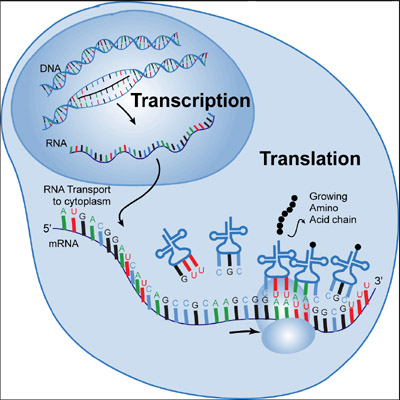
\includegraphics[scale=0.5]{illustrations/all.png}
\caption{From the initial DNA sequence to the protein\protect{\cite{imgAll}}}
\label{transcTransl}
\end{figure}

\begin{figure}[H]
\centering
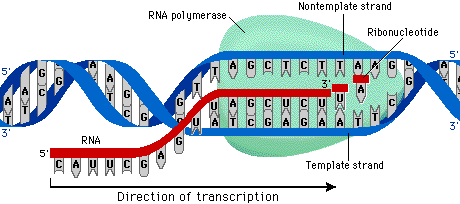
\includegraphics[scale=0.5]{illustrations/transcription.png}
\caption{Transcription of the DNA strand into mRNA\protect{\cite{imgTranscription}}}
\label{transcription}
\end{figure}

Once the transcription is performed, this molecule exits the cell nucleus, and later, during the translation (see Figure \ref{translation}), the RNA sequence is read by the ribosomes. The \textbf{ribosome} is a macro-molecule which associates an amino acid to each triplet of nucleotides -called \textbf{codon}. A protein is then the resulting sequence of amino acids.\\ 

It is worth noticing that mRNA is unstable\cite{brenner1961unstable} compared to DNA, that is, as a general rule, it cannot be read but a limited number of times by the ribosomes. Hence getting access to the sequence carried by a mRNA molecule provides a good idea of the number of produced proteins by the cell, thus of the cell activity and of the expressed genes; as opposed to the study of the DNA sequence, which can be considered rather as a identifying feature for a certain species or individual when compared to other organisms.\\ 

\begin{figure}[H]
\centering
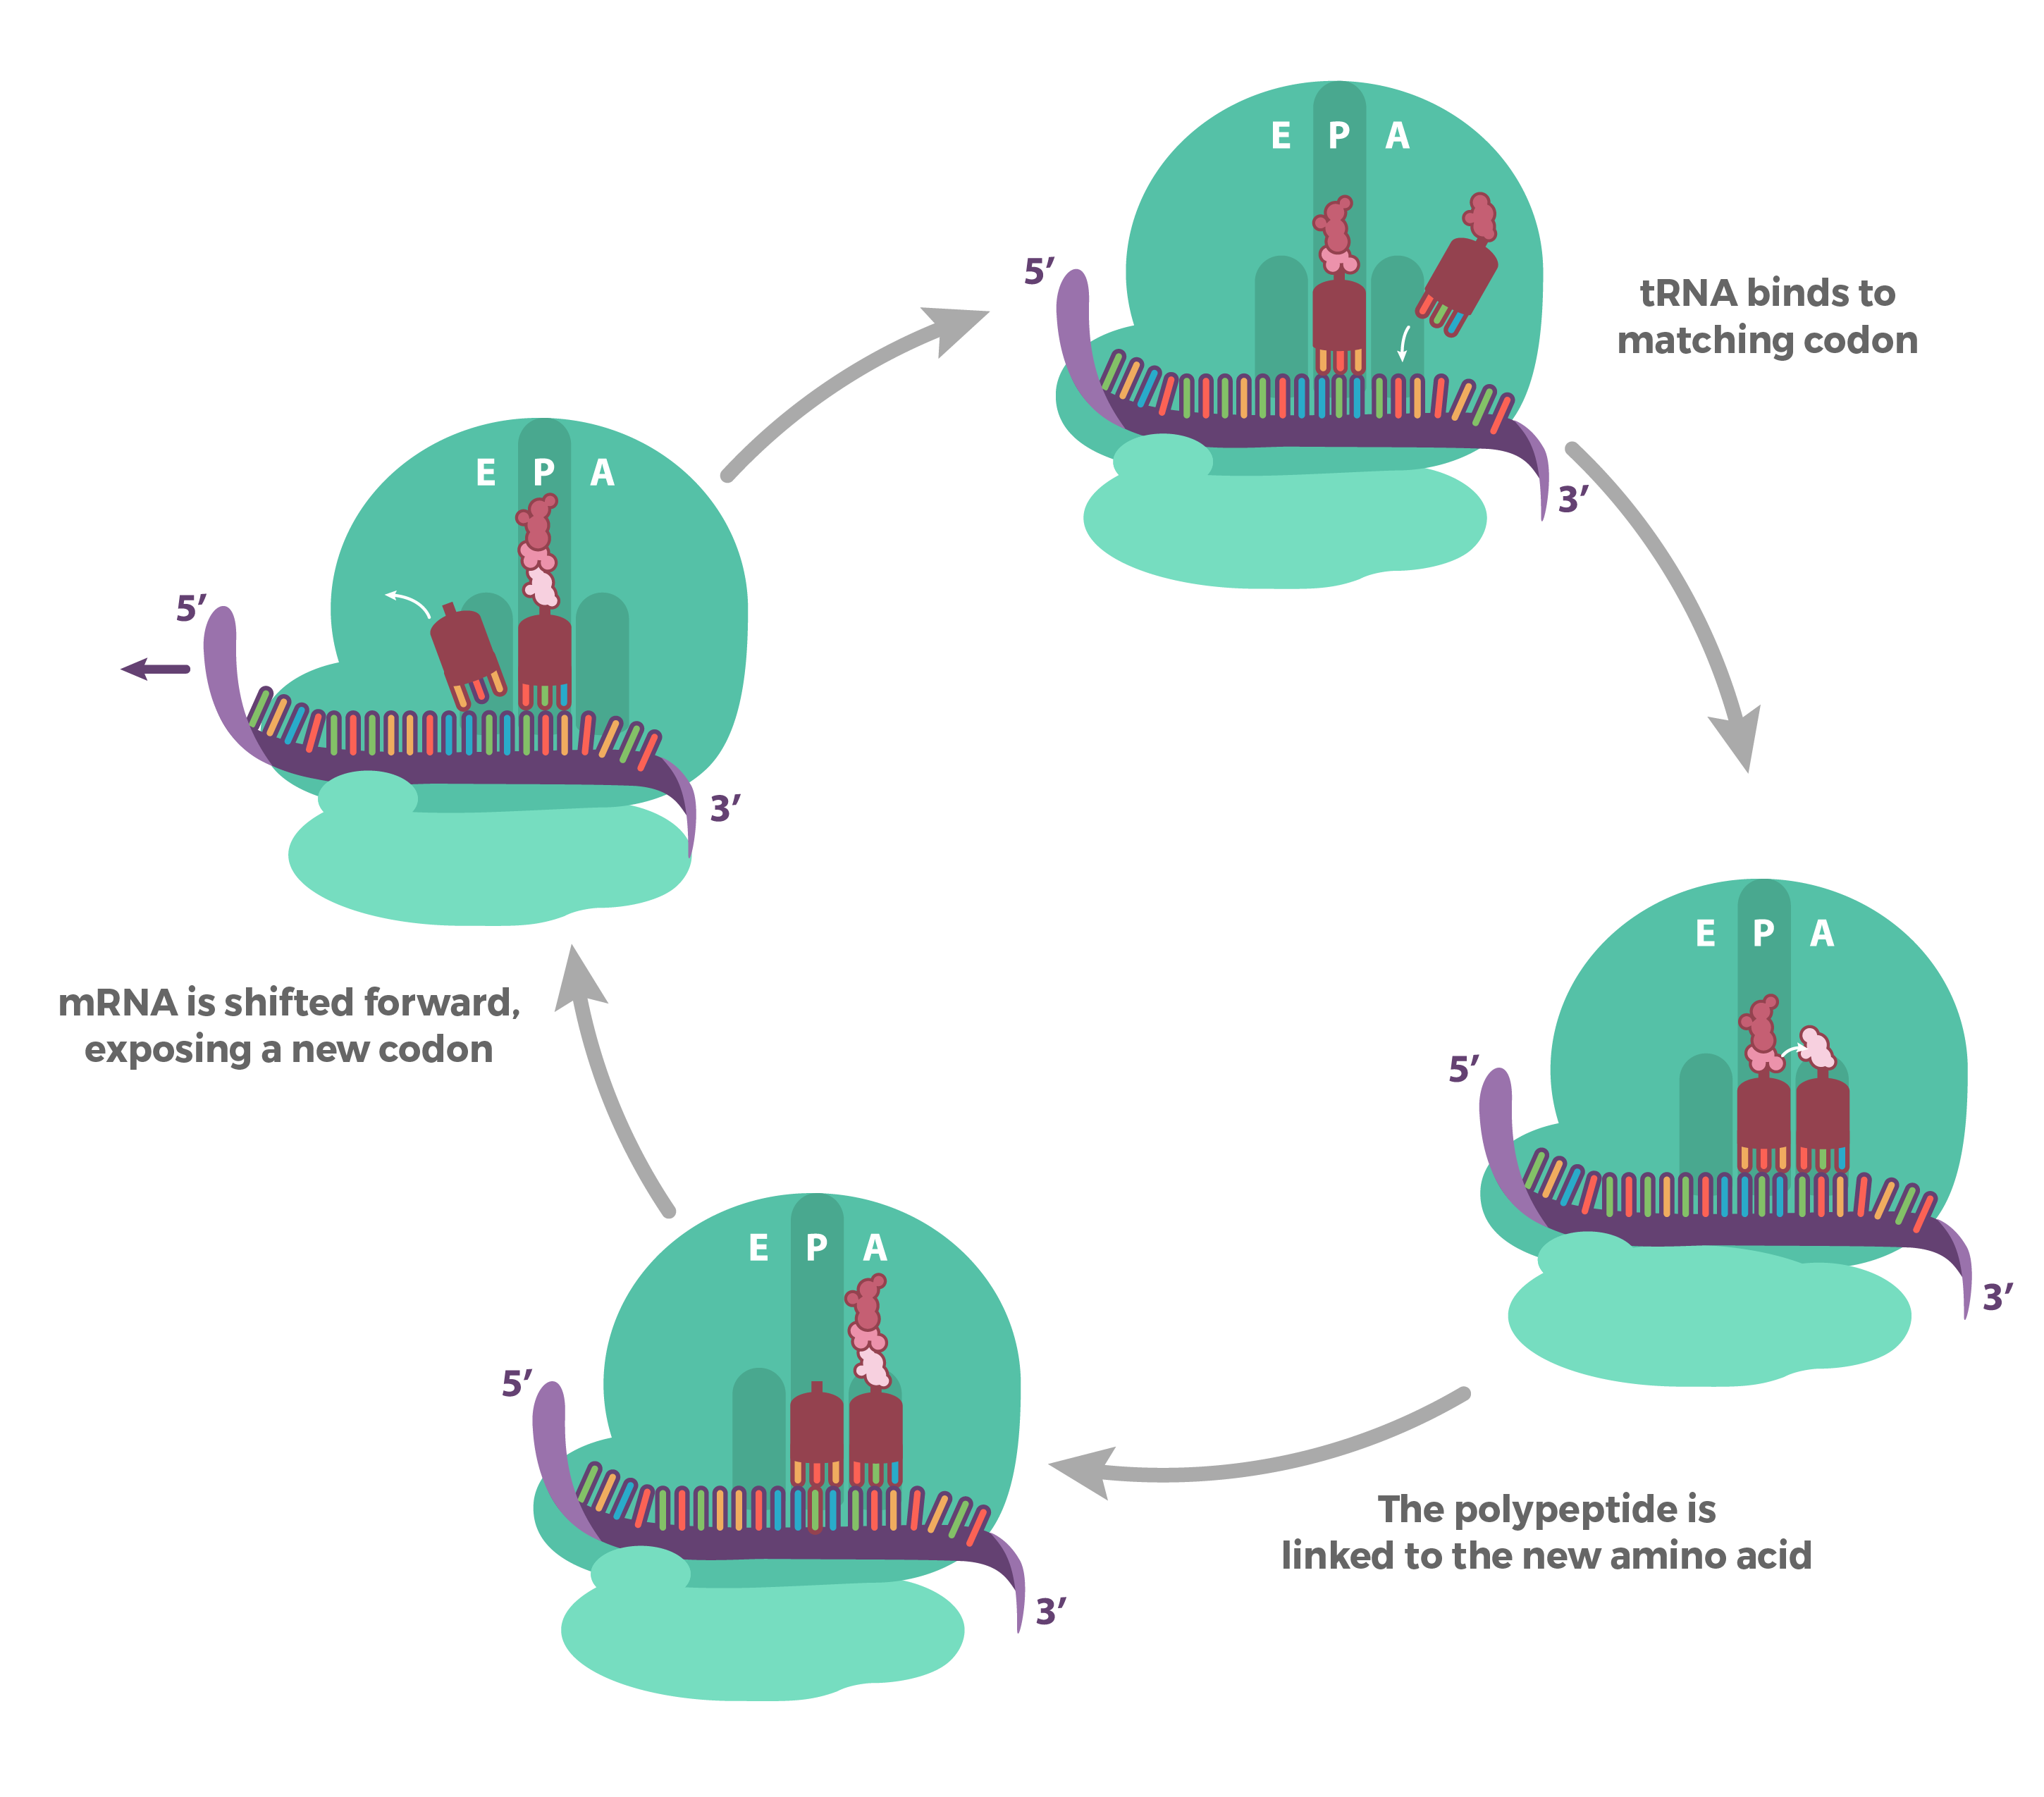
\includegraphics[scale=0.5]{illustrations/translation.png}
\caption{Translation of the mRNA into proteins\protect{\cite{imgTranslation}}. The green unit is the ribosome, and E, P and A are the three sites where translation occurs.}
\label{translation}
\end{figure}

A gene is considered expressed when the associated coding sequence is transcribed from the initial DNA sequence to the RNA sequence carried by the mRNA, because the protein it codes is likely to be produced by the ribosomes. 

\bigskip
\noindent \textbf{Cell clustering based on gene expression levels}
\bigskip

It is assumed that the levels of gene expression, for the different genes which coding sequences have been seen in the mRNA sequence extracted from a certain cell, determine the cell function in the organism.\\

The features which are the most discriminative in the grouping of cells, and which show a strong correlation with a given cell phenotype, are called \textbf{informative genes}\cite{liu2006efficient}.\\

For a given cell, the \textbf{gene expression pattern} is its profile of gene expression, which is assumed to be specific to a certain functional family of cells, i.e. cells having the same role in the organism (see \cite{barash2002context} for a discussion for this hypothesis).\\

Being able to find the informative genes, and to distinguish a gene expression pattern for each cell, can then provide a better insight of the cell organization in a certain species\cite{tintori2016transcriptional}, or of gene expression heterogeneity between different developmental stages\cite{goolam2016heterogeneity}, or a better understanding of the difference in cell activity between cancer-afflicted and healthy individuals\cite{ting2014single}, that may lead to the development of more efficient treatments, for instance.  Note that gene clustering based on gene expression levels exists too, and may use similar methods as cell clustering\cite{d2005does}\cite{jiang2004cluster}.\\

Hopefully, when a proper subset of informative genes has been selected, cells may be clustered according to their functional families or their cell type (see Figure \ref{cellclustering}). 

\begin{figure}[H]
\centering
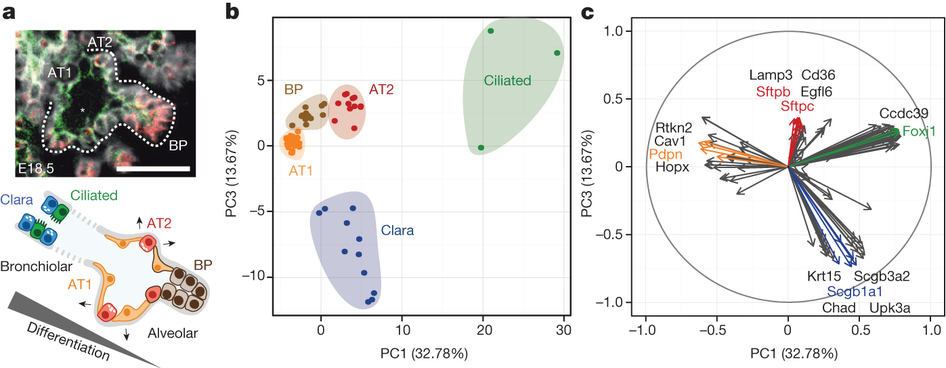
\includegraphics[scale=0.45]{illustrations/cellclustering.jpg}
\caption{Example of cell clustering based on gene expression data. Each cell functional family is represented by a distinct colour\protect{\cite{treutlein2014reconstructing}}}
\label{cellclustering}
\end{figure}

\section{About RNA sequencing}

\textbf{Purpose}
\bigskip

\textbf{RNA sequencing} is aimed at obtaining the \textbf{primary structure} of a certain RNA fragment, that is, the ordered series of letters A, G, C and U, which respectively refer to the following nucleotides: adenine, guanine, cytosine and uracil.\\

As explained above, most of the time, DNA and RNA sequencings serve different purposes. DNA sequencing allows to get access to the code needed for living things to survive, and may be helpful to retrace the evolutionary history of a given species, whereas RNA sequencing can cast a light on the regulatory inter-gene interactions (has gene A an influence on the expression level of gene B? Does it favour/inhibit the transcription of this gene?) and on the developmental phase of an organism, from the fertilized egg to the fetus: how do the different limbs form? How do some stem cells turn into specialized cells, having only a very specific function in the organism? (This phenomenon is called \textbf{cell differentiation}.) However, how regulatory systems exactly work is still unknown, and DNA may be useful in the future to understand whole regulatory processes.

\begin{figure}[H]
\centering
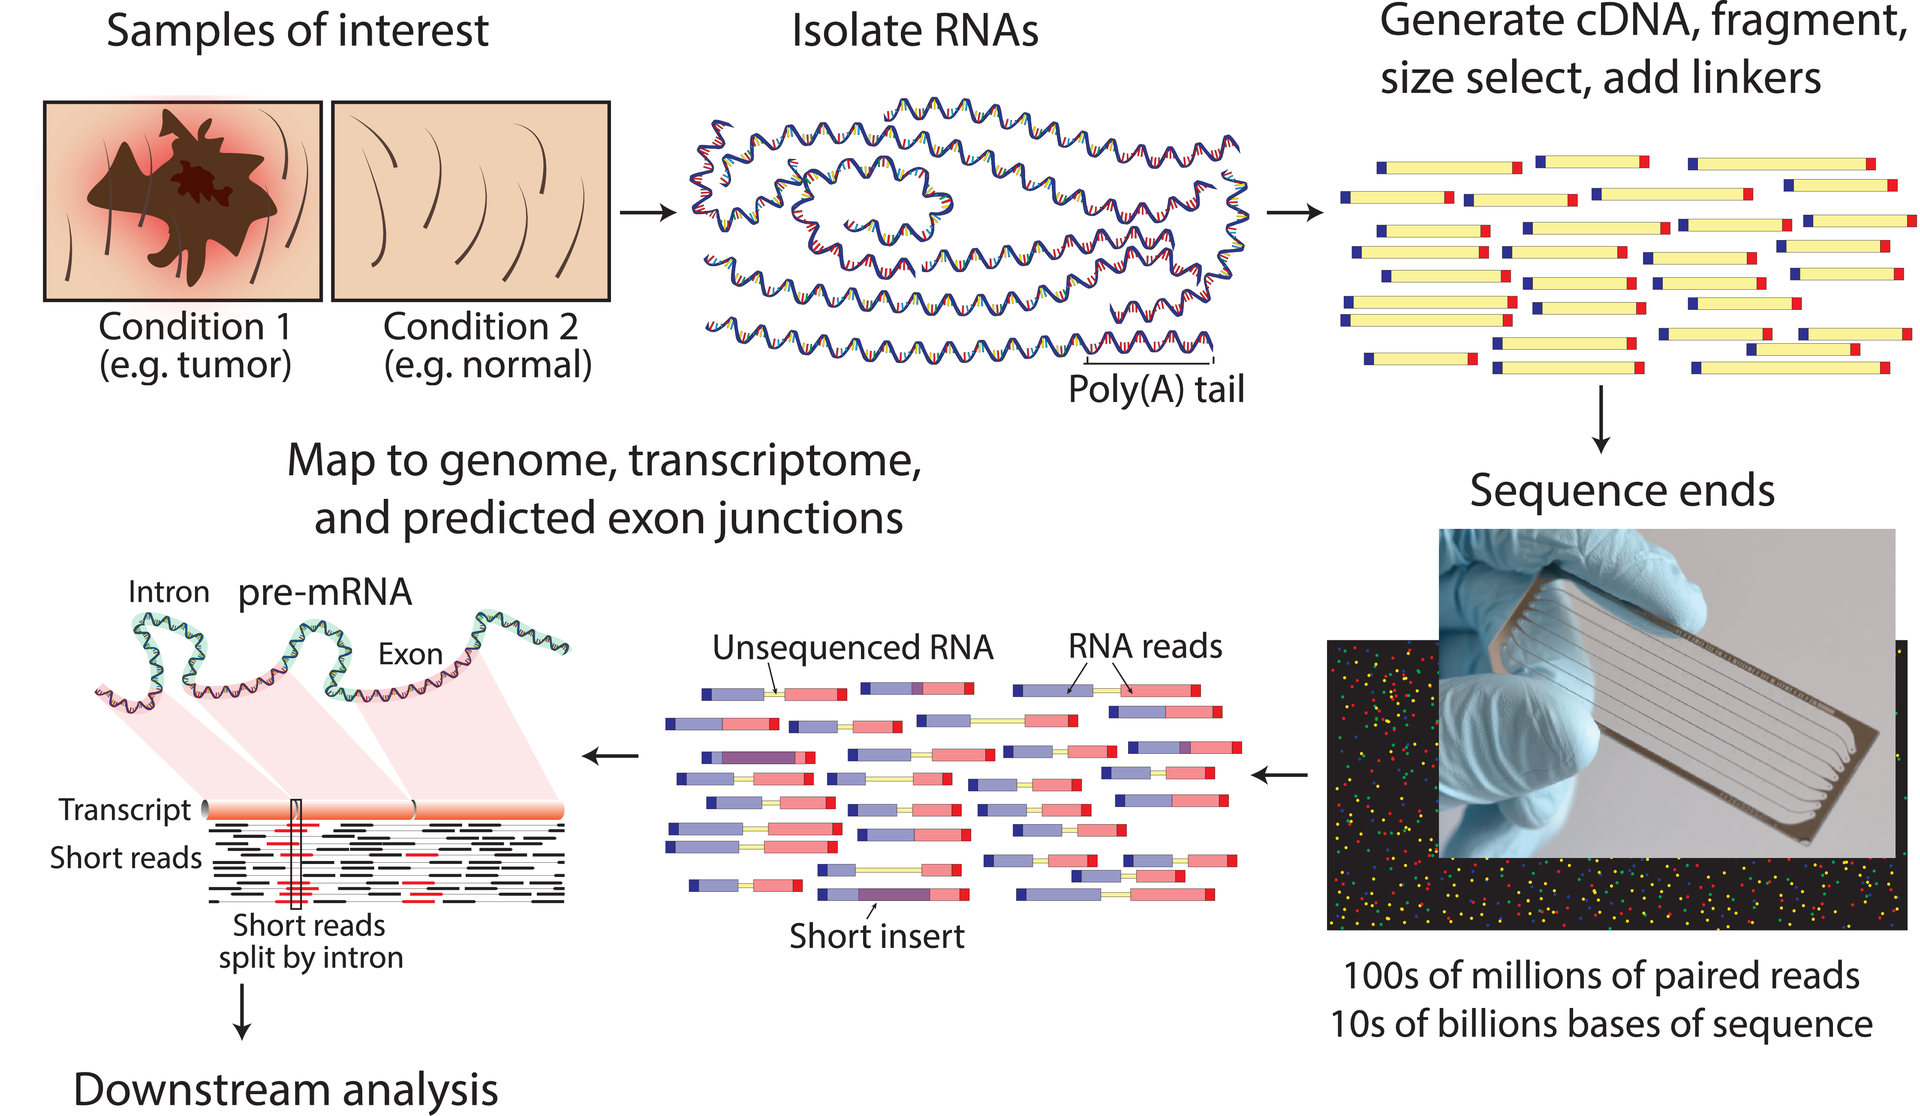
\includegraphics[scale=1.5]{illustrations/sequencing.png}
\caption{General pipeline to get a gene expression matrix from a mRNA fragment\protect{\cite{griffith2015informatics}}}
\label{sequencing}
\end{figure}

Sequencing biological material requires several steps (see Figure \ref{sequencing}).\\

\begin{enumerate}
\item First, the mRNA molecule in the samples are chemically isolated. 
\item Then, these molecules are used to generate (complementary) DNA (cDNA) via \textbf{reverse-transcription}. 
\item Later, these cDNA strands are fragmented into \textbf{reads}. Reads are short series of A (which stands for adenine), G (guanine), C (cytosine) and T (thymine) letters resulting from the sequencing of the mRNA strand. Then these reads are sequenced, and the resulting reads are aligned to a reference genome (see Figure \ref{alignment}), that is available in a online database such as \textsc{WormBase}\cite{stein2001wormbase} or \textsc{NCBI}\cite{ncbi}, for instance. The best alignment is the one that preserves most the order of the bases in the reference sequence -but the exact definition of the "best alignment" highly depends on the alignment algorithm used. 
\item Then a gene expression matrix M is computed: each time a read from condition $j$ is aligned to a certain reference sequence corresponding to a specific gene $i$, the associated number $M_{i,j}$ is incremented.
\end{enumerate}

Gene expression value is also called \textbf{gene expression level}, or \textbf{gene expression count} -when the numbers are integers. The data to analyze is then the integer matrix of gene expression value, that is, as a general rule, a matrix M which rows are indexed by the considered genes -or \textbf{features}- and which columns are indexed by the studied cells -called \textbf{samples}. Columns can also be called \textbf{conditions} (e.g., non-cancer versus cancer cells, or treatment A versus treatment B versus treatment C), depending on the study. Each coefficient $M_{i,j}$ is the number of times the coding sequence for gene $i$ has been recognized in the resulting ${A, G, U, C}$-sequence obtained by the sequencing of the mRNA stand in cell $j$, that is, the number of detected reads in the sequencing of this mRNA strand that refer to this gene.\\

However, the total number of reads detected may vary from one cell or condition to another. In order to be able to compare gene expression values across several cells, the matrix may be trimmed (to remove outlier cells or genes), and "normalized" to preserve proportionality between gene expression values. There are actually many ways to achieve this normalization\cite{love2014moderated}\cite{chen2014differential}.

\begin{figure}[H]
\centering
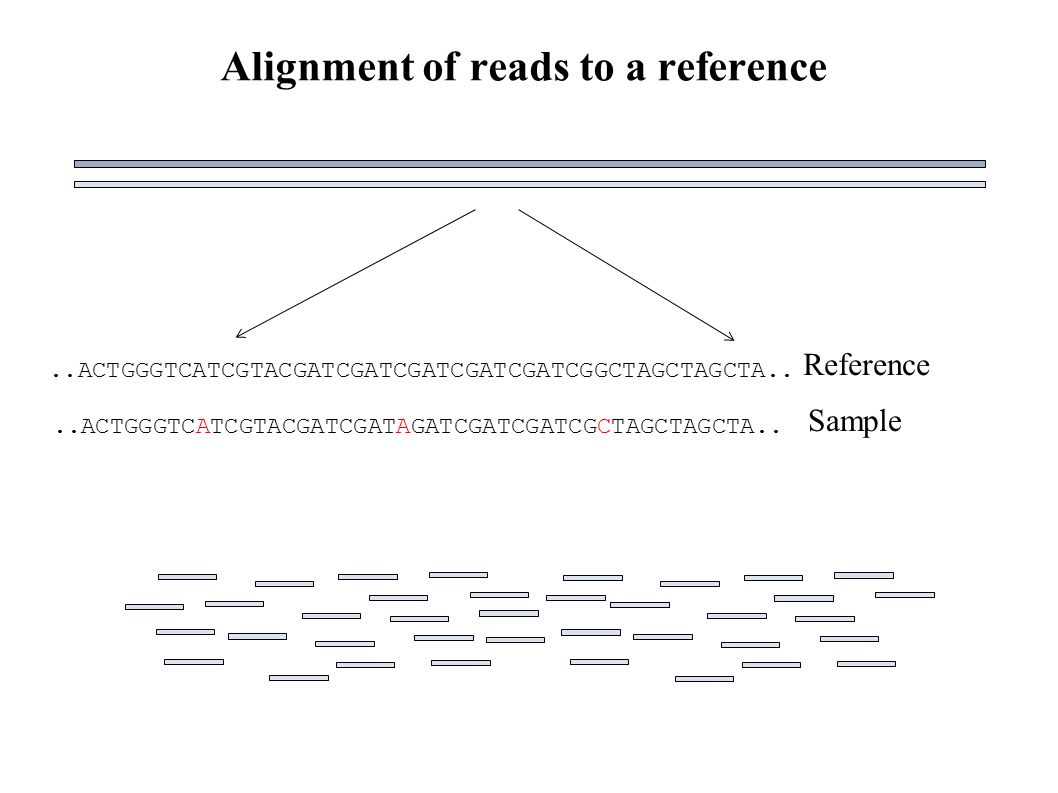
\includegraphics[scale=0.45]{illustrations/alignment.jpg}
\caption{Read alignment\protect{\cite{imgAlignment}}}
\label{alignment}
\end{figure}

My implementation of a pipeline to get a count matrix from a set of bulk RNAseq reads (Illumina sequence data, contained in one or two .fastq file-s), provided a reference genome (.fasta file) and the corresponding annotation file (.gtf), is available there: {\url{https://github.com/oist-gene-clustering/RNAseqpipeline}}\\ 

\bigskip
\noindent \textbf{About single-cell RNA sequencing (scRNAseq)}
\bigskip

scRNAseq is quite a new technology. At first, studying mRNA became affordable thanks to microarrays\cite{chang1983binding}, that started to be widely used in 1995\cite{schena1995quantitative}. This technology used miniaturized and optimized high-throughput screening on arrays of biological data\cite{microarraywiki} (see Figure \label{microarray}). The latter were also used for DNA studies ("DNA microarrays"\cite{southern2001dna}). 

\begin{figure}[H]
\centering
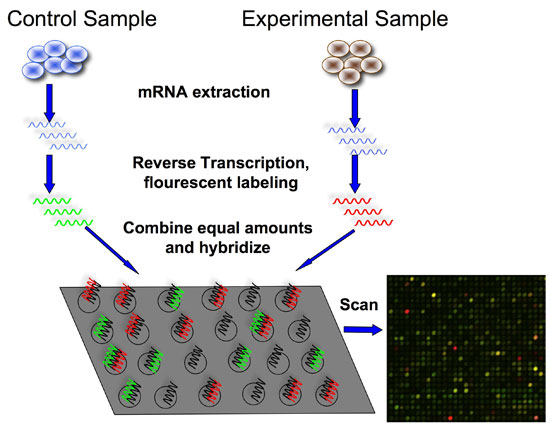
\includegraphics[scale=0.5]{illustrations/microarray.jpg}
\caption{Microarray experiment for mRNA data\protect{\cite{imgMicroarray}}}
\label{microarray}
\end{figure}

At this time, tools for improving downstream analysis (that is, the analysis of the resulting gene expression matrix) were needed, and many clustering algorithms\cite{do2008clustering}\cite{dabney2005classification}\cite{eisen1998cluster}\cite{monti2003consensus} and statistical tools\cite{simon2007analysis}\cite{kerr2000analysis} were designed.\\

However, in 2007, \cite{barbazuk2007snp} used RNA-sequencing to detect chromosomal modifications in the transcriptome, via \textbf{reverse transcription} (see previous section). Because of its assets, comparing to microarrays -increased data quality\cite{zhao2014comparison}\cite{wang2009rna}, improved detection of rare transcripts, ...\cite{illuminarnamicroarray}- and the drop in the sequencing price, researchers' interest in regular or bulk RNAseq had soon plummeted in the 2010's and until now\cite{conesa2016survey}\cite{leon2015bayesian}.\\

Until quite recently, only groups of cells could be isolated and sequenced. Henceforth, the gene expression levels obtained actually were average gene expression values across the cells from one given group. Thanks to scRNAseq, cell activity can now be witnessed at a higher resolution, thus give a more accurate report of the gene expression in a given single cell\cite{stegle2015computational}\cite{poirion2016single}. Nevertheless, there is doubt about the reusability of the previous methods and tools developed for RNA-seq and microarrays, due to the following phenomena being specific to single-cell RNA seq data:\\

\begin{itemize}
\item scRNAseq data are even noisier than bulk RNA seq, because of the low biological material available and procedures which can easily be contaminated\cite{brennecke2013accounting}\cite{grun2014validation}.
\item Unlike bulk RNAseq data, scRNAseq results are subject to \textbf{dropout} phenomena\cite{kharchenko2014bayesian}\cite{lun2016pooling}: a lot of gene transcripts cannot actually be detected (because of an error during reverse-transcription), which results in a gene expression matrix with a lot of zeros, and makes transcriptome profiling harder to perform.
\item The higher resolution offered by single-RNA sequence provide a new insight on cells having a same cell type: the gene expression levels of certain genes may vary from one cell to another\cite{poirion2016single}\cite{martinez2017aging}.
\item It also allows to observe the evolution of cell gene expression profiles during \textbf{mitosis} (cell cycle)\cite{trapnell2014dynamics}. The mitosis is the cell division into two new cell copies.

\end{itemize} 

Today, there are lots of techniques\cite{shapiro2013single} for single-cell RNA sequencing, the first one being Tang et al.\cite{tang2009mrna} (2009), see Figure \ref{historyseq}.

\begin{figure}[H]
\centering
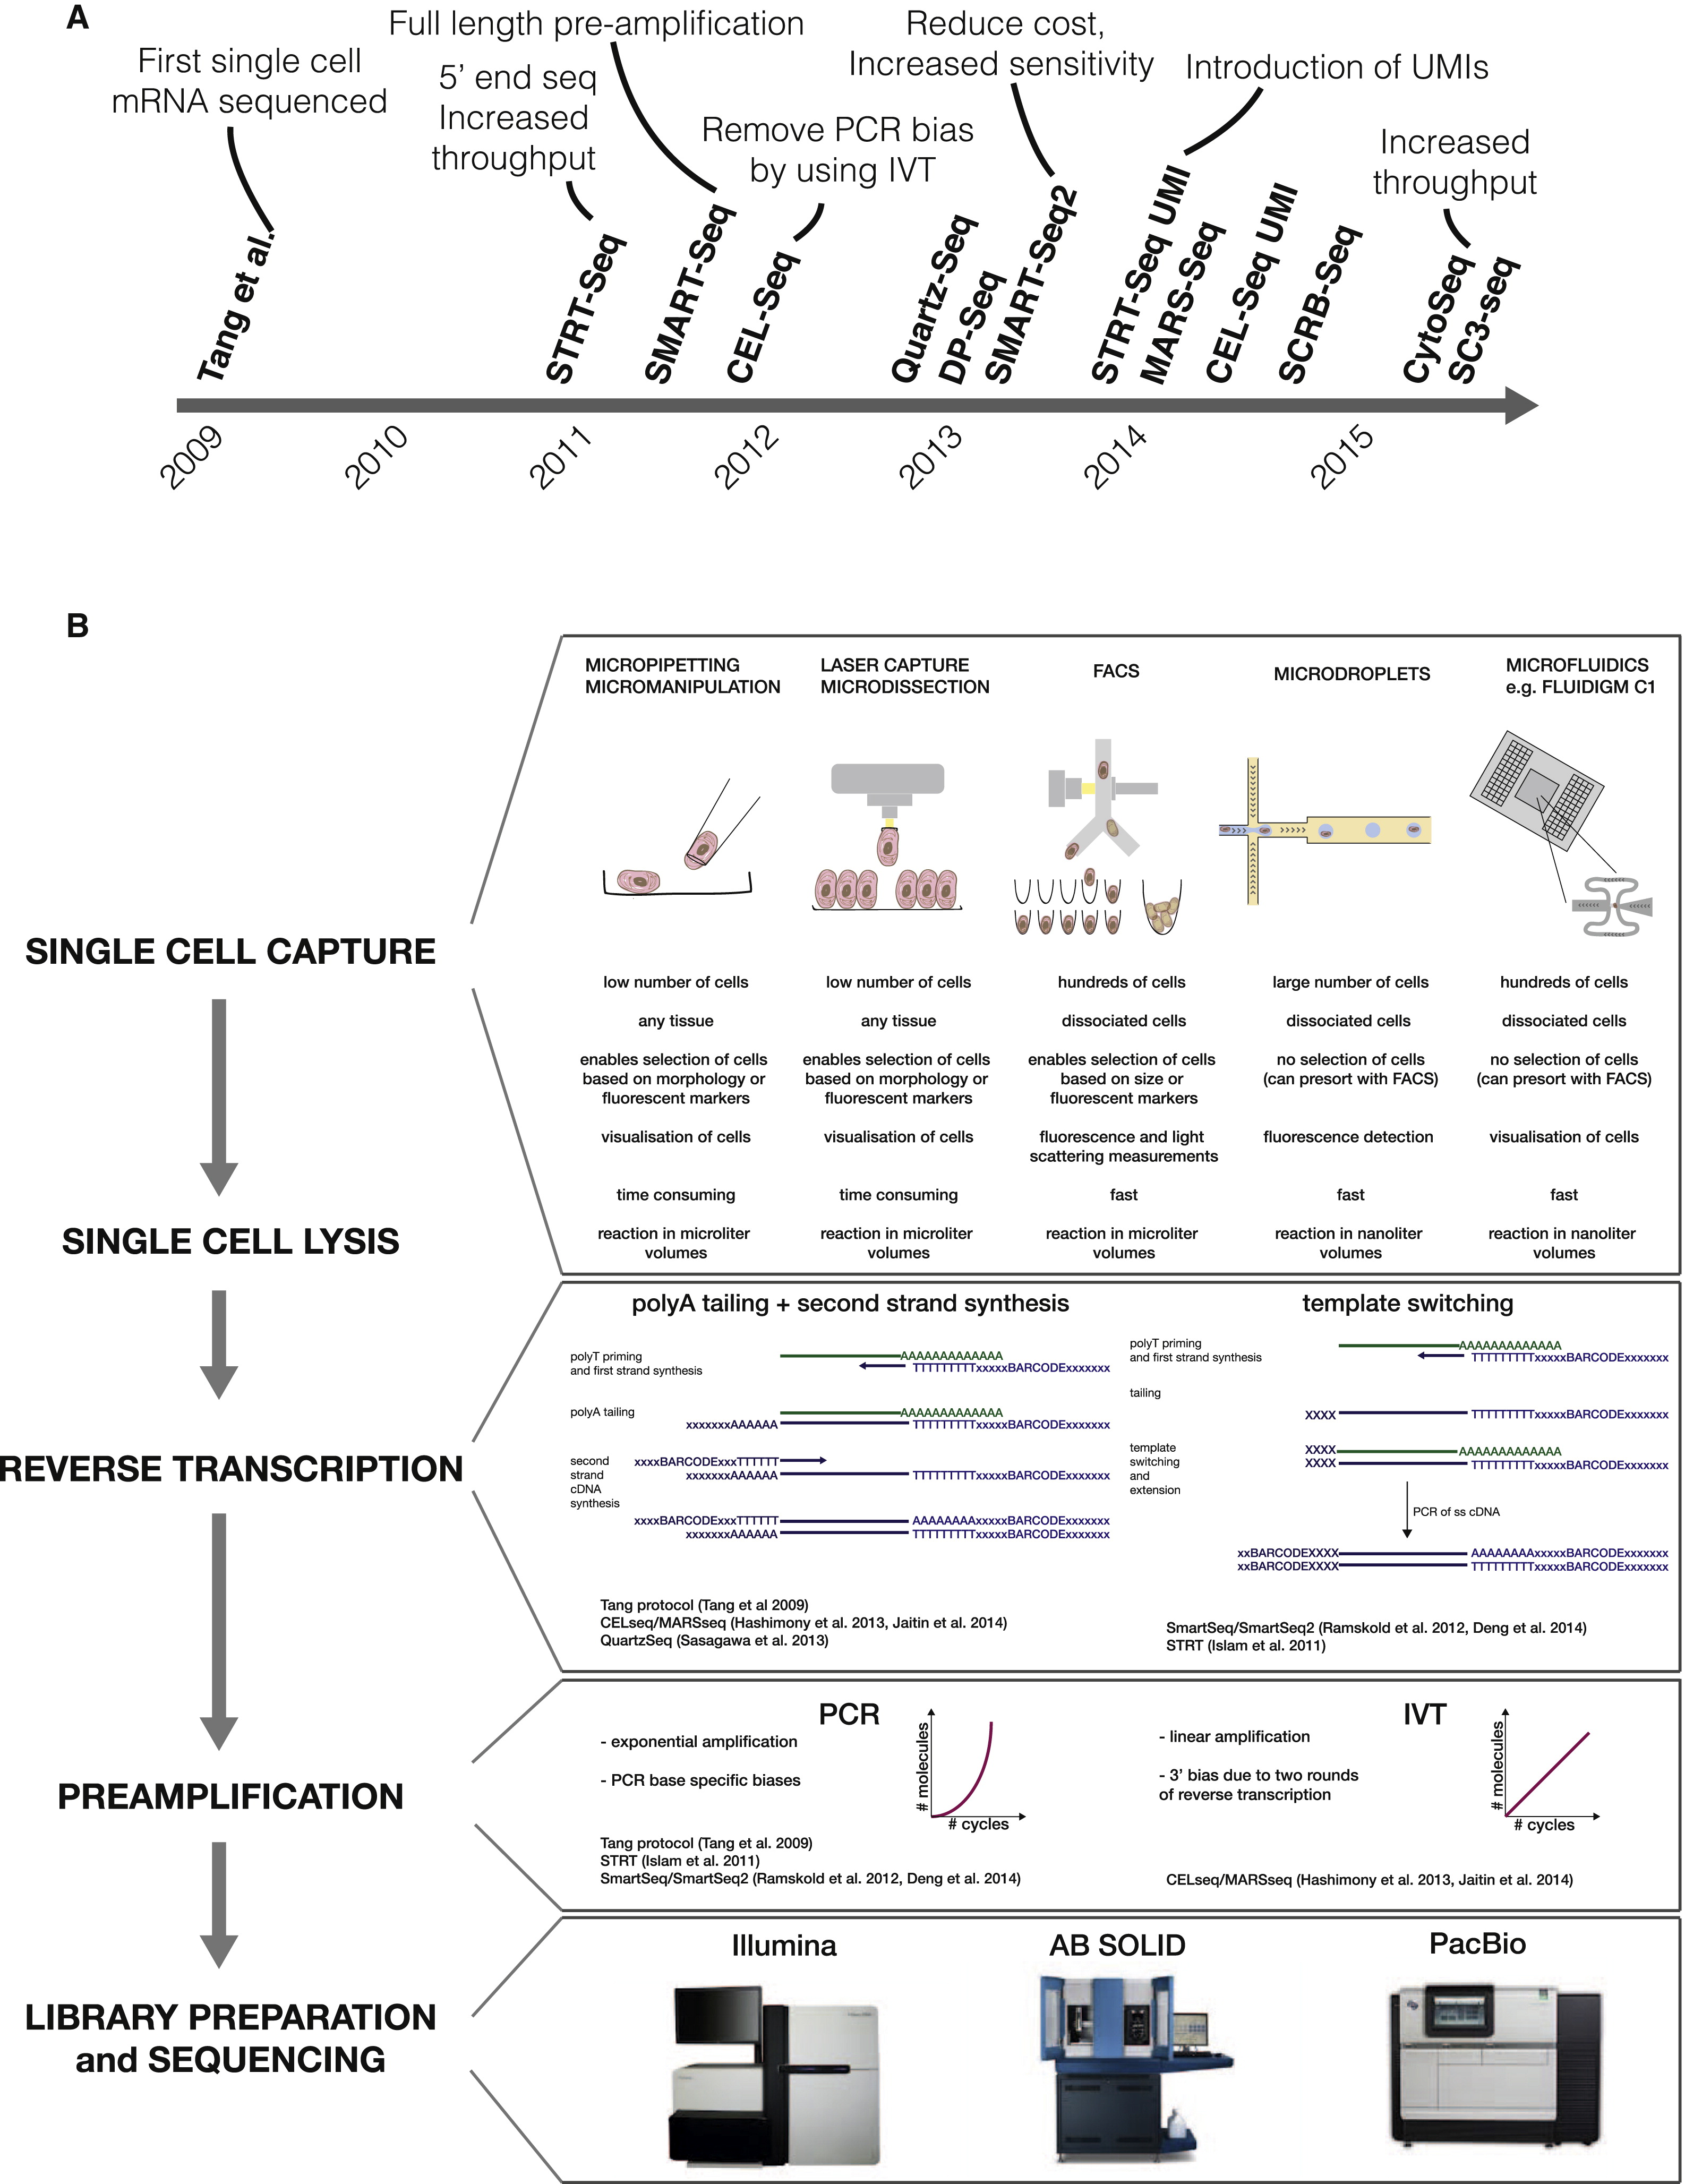
\includegraphics[scale=1]{illustrations/scrnaseq.jpg}
\caption{History of scRNAseq and general pipeline to get a set of reads from a single-cell RNA fragment\protect{\cite{kolodziejczyk2015technology}}}
\label{historyseq}
\end{figure}

My implementation of a pipeline to get a count matrix from a set of scRNAseq reads (Illumina sequence data, contained in one or two .fastq file-s), provided a reference genome (.fasta file) and the corresponding annotation file (.gtf), is available there: {\url{https://github.com/oist-gene-clustering/RNAseqpipeline}}\\

It uses softwares from \cite{andrews2010fastqc}\cite{bolger2014trimmomatic}\cite{langmead2012fast}\cite{li2009sequence}\cite{pertea2015stringtie}\cite{jiang2016quality}\cite{katayama2013samstrt}\cite{trapnell2012differential}.

\section{Cluster analysis}

\textbf{Purpose}
\bigskip

\textbf{Cluster analysis}, that is, grouping data samples respect to their similarity -same-group samples are more similar in some sense than to samples from other groups- is one of the primary steps for exploring data, and is meant to guide further analysis. Applied to scRNAseq, it may help discovering new cell functional families\cite{jiang2016giniclust}, control data quality\cite{mccarthy2016scater} and delete outlier samples\cite{kiselev2016sc3}, or better understand cell differentiation at a given developmental stage\cite{goolam2016heterogeneity}.\\

The different groups -called \textbf{clusters}- are not known beforehand, neither are the features that can the most reliably discriminate the data samples. As a general rule, data samples are identified to vectors, where each component refers to a certain feature, that may be binary, real-valued, categorical, ... according to the type of data. Thus cluster analysis -also called clustering- boils down to grouping points in a certain mathematical space.\\

\begin{figure}[H]
\centering
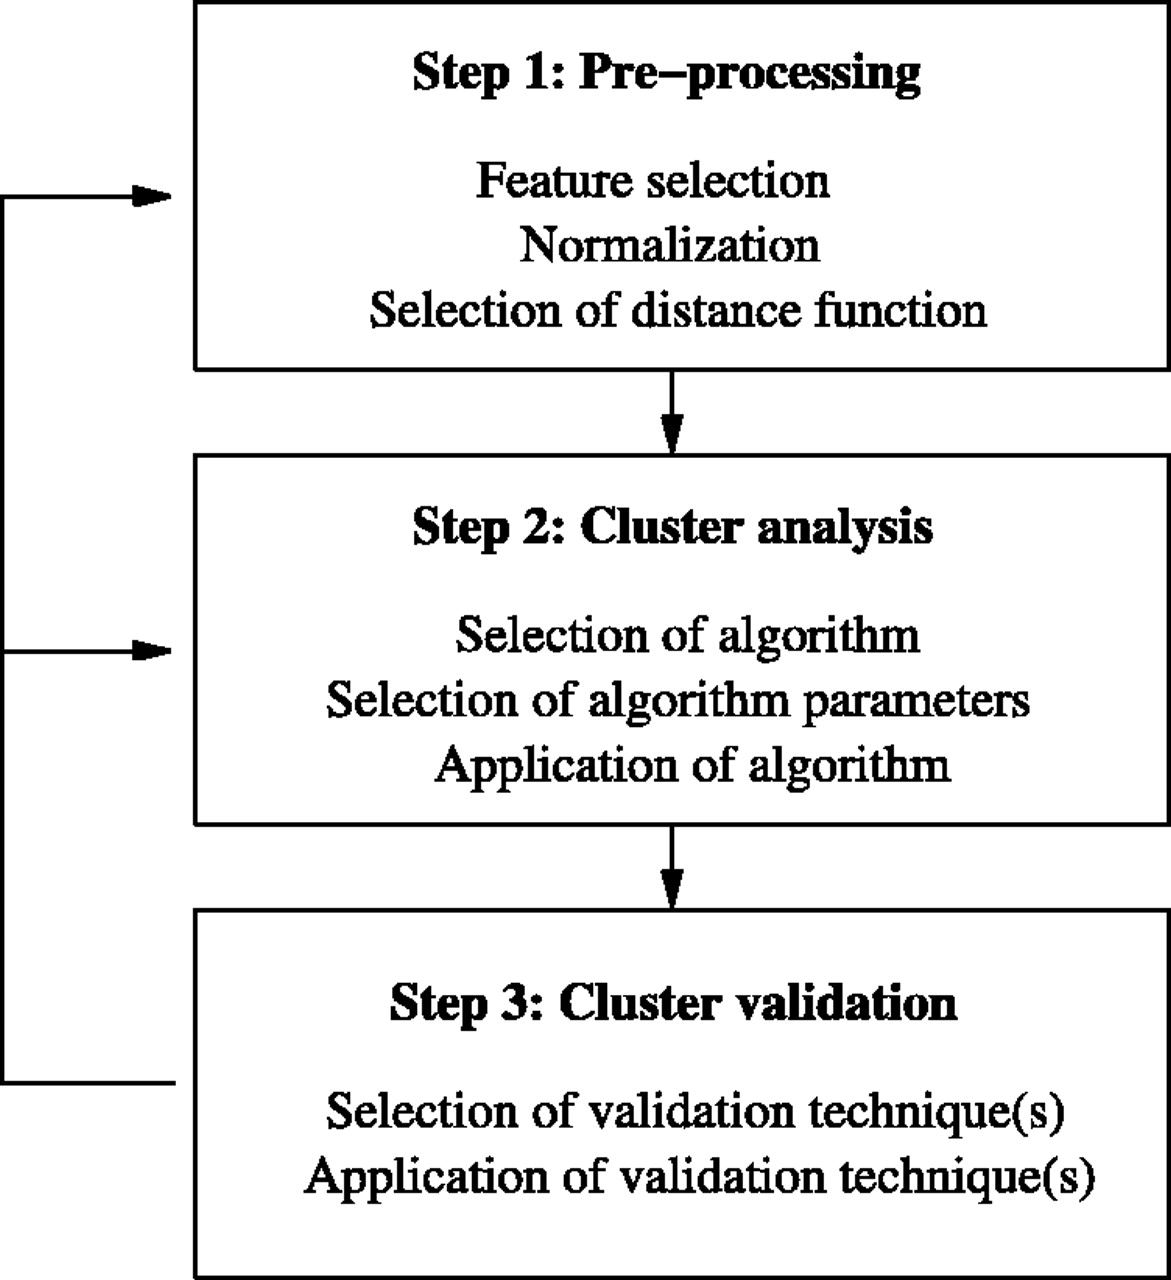
\includegraphics[scale=0.15]{illustrations/clusteranalysis.jpg}
\caption{Pipeline of cluster analysis, from the raw data to the clustering validation\protect{\cite{handl2005computational}}}
\label{clusteranalysis}
\end{figure}

\begin{table}[H]
\centering
\begin{tabular}{| l | l | l |}
\hline
\parbox[c]{5cm}{\textbf{Steps}} & \
\parbox[c]{5cm}{\textbf{Selection of the\\ following items}} & 
\parbox[c]{5cm}{\textbf{Corresponding questions}}\\
\hline
\parbox[c]{5cm}{\textbf{Pre-processing}} & 
\parbox[c]{5cm}{Feature selection,\\distance selection,\\data points normalization} & 
\parbox[c]{5cm}{\textit{~\\- What is the data about?\\- What are the relevant data features, and how to efficiently extract them?\\- Do I need to perform some transformations on the data points before comparing their vectors?\\- How do I compare data vectors?\newline}}\\
\hline
\parbox[c]{5cm}{\textbf{Clustering}} & 
\parbox[c]{5cm}{Choice of the algorithm \\(and of corresponding\\ parameters)} & 
\parbox[c]{5cm}{\textit{~\\- How do I efficiently get the clusters?\\- What is the algorithm input?\newline}}\\
\hline
\parbox[c]{5cm}{\textbf{Clustering\\validation}} & 
\parbox[c]{5cm}{Internal/external measures} & 
\parbox[c]{5cm}{\textit{~\\- How do I check if the clusters are consistent with the original data (external measures)?\\- How do I check if the algorithm went wrong (internal measures)?\newline}} \\
\hline
\end{tabular}
\caption{Cluster analysis steps (according to \cite{handl2005computational})}
\label{clustersteps}
\end{table}

Clustering is not all about applying a certain algorithm to the data (see Figure \ref{clusteranalysis} and Table \ref{clustersteps}). Each step above is of equal importance. More especially, validation step is of paramount importance, since there is no clustering algorithm that will be able to predict the best grouping of points for any kind of data -with more than 2 points\cite{kleinberg2002impossibility}. The choice of the algorithm may determine the shape of the resulting clusters (e.g. spherical for K-means), their size and their density, for instance. Thus having an idea of the clustering error can be helpful.\\

Moreover, feature selection, especially for gene expression clustering,  is also a critical step. Since only a handful of genes are really informative, that, provide insight on the cell functional family, the remaining of the features is but noise, thus useless, and may also prevent an algorithm to find the patterns. There is currently no common definition of what an informative gene should be, and many methods exist\cite{hira2015review}\cite{jirapech2005feature}\cite{latkowski2014feature}. Most of the time, a gene is considered informative if the variance of its expression across the cells is high, and if they are considered independent -this leads to the use of PCA on the gene expression matrix. However, PCA actually limits the number of informative genes to the minimum of the dimensions of the gene expression matrix $M$ (because the loading vectors it computes are the eigenvectors of $M^{T}M$, in increasing corresponding eigenvalue order), and assumes a linear relationship between the gene expression values\cite{pearson1901liii], so this definition is not really satisfying. Plus, the variance of gene expression may be due to a dropout event. Other algorithms select the features according to their frequency in the gene expression matrix\cite{kiselev2016sc3}: ubiquitous genes are removed, because they are considered poorly specific, rare genes can be seen as noise, or, if a certain gene appear in only a few cells or with a low expression value, it may be also removed. However, this approach may prevent the algorithm to find rare cell types for instance\cite{kiselev2016sc3}. To my mind, informative genes are features with non-null variance, frequency in cells inferior to a certain threshold (typically, less than 70\% of the cells), and such as the (positive or negative) correlation between two informative genes is less than a certain threshold (for instance, 0.9). This quite intuitive definition is actually used in the \textbf{caret} package\cite{kuhn2008caret}, among other softwares, and also described in \cite{guyon2003introduction}. I could not actually find a convincing non-parametric definition. The limit on the frequency actually removes all the quality control genes. The correlation function chosen may be a rank correlation function such as Kendall's $\tau$\cite{kendall1938new}, to avoid the caveats of the Pearson correlation measure, for instance, sensibility to outliers\cite{outliercorr}.

\begin{definition}[Kendall's $\tau$]\label{kendalltau}{Let $n \in \mathbb{N}^*$, X = \{$x_1, x_2, ..., x_n$\} and Y = \{$y_1, y_2, ..., y_n$\}, such as X and Y have unique orderable values.\\

Let $a$ denote the number of pairs $(x_i, y_i), (x_j, y_j), i,j \in \{1,2, ..., n\}$ such as $x_i <  x_j \land y_i < y_j$ OR $x_i >  x_j \land y_i > y_j$, and $b$ denote the number of pairs such as $x_i <  x_j \land y_i > y_j$ OR $x_i >  x_j \land y_i < y_j$. Then:

\begin{center} $\tau = \frac{a-b}{\frac{1}{2} \times n \times (n - 1)}$ \end{center}}\end{definition}

\newpage

\bigskip
\noindent \textbf{State-of-the-art}
\bigskip

Several different methods have been designed for clustering (sc)RNAseq (see Tables \ref{methods} and \ref{methods2}).

\begin{table}[H]
\centering
\begin{tabular}{| l | l | l | l |}
\hline
\parbox[c]{5cm}{\textbf{Category}} & 
\parbox[c]{5cm}{\textbf{Description}} &
\parbox[c]{5cm}{\textbf{Implementations}}\\
\hline
\parbox[c]{5cm}{\textbf{Connectivity-based}} & 
\parbox[c]{5cm}{~\\ These algorithms build a hierarchy of the samples (i.e. a tree which leaves are the samples), according to the chosen distance measure.\\

Given a height, the final clustering is the set of trees in the forest obtained by deleting edges higher than the selected height. \newline} &
\parbox[c]{5cm}{Hierarchical clustering\\(SINCERA\cite{guo2015sincera}), ...}\\
\hline
\parbox[c]{5cm}{\textbf{Centroid-based}} & 
\parbox[c]{5cm}{~\\ Given the expected number of clusters $k$, these algorithms compute iteratively $k$ points, such as each of them 
is the centroid of a set of similar points.\\ 

The final clustering is obtained by assigning each point to the cluster of the nearest centroid. These steps are repeated until convergence of the clusters.\newline} &
\parbox[c]{5cm}{K-means\cite{macqueen1967some}\cite{tseng2007penalized},\\

Fuzzy C-means\cite{dunn1973fuzzy}\cite{filippone2005unsupervised},\\

Nonnegative Matrix\\ Factorization\cite{lee1999learning}\\(e.g. NIMFA\cite{shao2016robust}),\\

Nearest Neighbor-like\\(e.g. SNN-Cliq\cite{xu2015identification}), ...}\\
\hline
\parbox[c]{5cm}{\textbf{Density-based}} & 
\parbox[c]{5cm}{~\\ Clusters are areas of higher density (in the number of data points) compared to the remainder of the data points.\\

These algorithms try to detect local differences in density in order to find the clusters.\newline} &
\parbox[c]{5cm}{DBSCAN\cite{ester1996density}, ...}\\
\hline
\end{tabular}
\caption{Some categories of clustering algorithms with examples from gene expression clustering (1) (adapted from \cite{classifclustering})}
\label{methods}
\end{table}

\begin{table}[H]
\centering
\begin{tabular}{| l | l | l | l |}
\hline
\parbox[c]{5cm}{\textbf{Distribution-based}} & 
\parbox[c]{5cm}{~\\ A mixture of $k$ same-model distributions (where $k$ is the expected number of clusters) is fitted to the data, that is, the different parameters of the mixture are such as they maximize the likelihood of the observed data.\\

Then the probability of membership of each point to every cluster is computed, and the final clustering is the one maximizing the membership probabilities.\newline} &
\parbox[c]{5cm}{Gaussian Mixture Models\\ (e.g. EMCluster\cite{melnykov2009model},\\MCLUST\cite{fraley1999mclust}),\\

\textit{ad hoc} models (e.g. Seurat\cite{satija2015spatial}), ...}\\
\hline
\parbox[c]{5cm}{\textbf{Discriminative feature\\computation}} & 
\parbox[c]{5cm}{~\\These algorithms first compute a somehow summary of the most relevant features of each point, either
by representing them by the restrictions of their associated vectors to the components having the maximum of variance (PCA), or
by mapping the data vectors to 2D (resp. 3D) vectors such as the 2D (resp. 3D) representations of two similar vectors in the 
original space are close in the new space (t-SNE).\\

Then one of the algorithms above is applied to the resulting representations.\newline} &
\parbox[c]{5cm}{Principal Component Analysis (e.g. pcaReduce\cite{yau2016pcareduce}),\\

t-Stochastic Neighbor Embedding\\
(e.g. t-SNE+K-means\cite{grun2015single},\\
t-SNE+DBSCAN), ...}\\
\hline
\parbox[c]{5cm}{\textbf{Consensus clustering}} & 
\parbox[c]{5cm}{~\\After having selected one of the algorithms described, and iterated it several times with different values of parameters, these algorithms construct a 
consensus matrix $M$ such as: $M_{i,j}$ is the (mean) number of times points i and j are located in the same cluster.\\

$M$ is then used to determine the final clustering.\newline} &
\parbox[c]{5cm}{e.g. SC3\cite{kiselev2016sc3}, ...}\\
\hline
\end{tabular}
\caption{Some categories of clustering algorithms with examples from gene expression clustering (2) (adapted from \cite{classifclustering})}
\label{methods2}
\end{table}

\chapter{scRNAseq analysis application}

Along with scRNAseq, huge amounts of gene expression data are available. Especially for newly-scRNA-sequenced species, such as \textit{Ciona intestinalis}\cite{suyama2016singlecell} or \textit{Caenorhabditis elegans}\cite{tintori2016transcriptional}, one would like to \textit{explore} the data, that is, being able to visualize the genes and cells that are the most informative about a certain condition, observe the cell correlation depending on certain selected genes of interest, distinguish genes that are the most discriminative between cell functional families or conditions (this is \textbf{differential expression analysis}), etc. This is a part of the downstream analysis that can be performed on the gene expression matrix obtained after sequencing.

\begin{figure}[H]
\caption{\textit{Ciona intestinalis}\protect{\cite{imgCiona}} (left) and \textit{Caenorhabditis elegans}\protect{\cite{imgCelegans}}}
\centering
\subfigure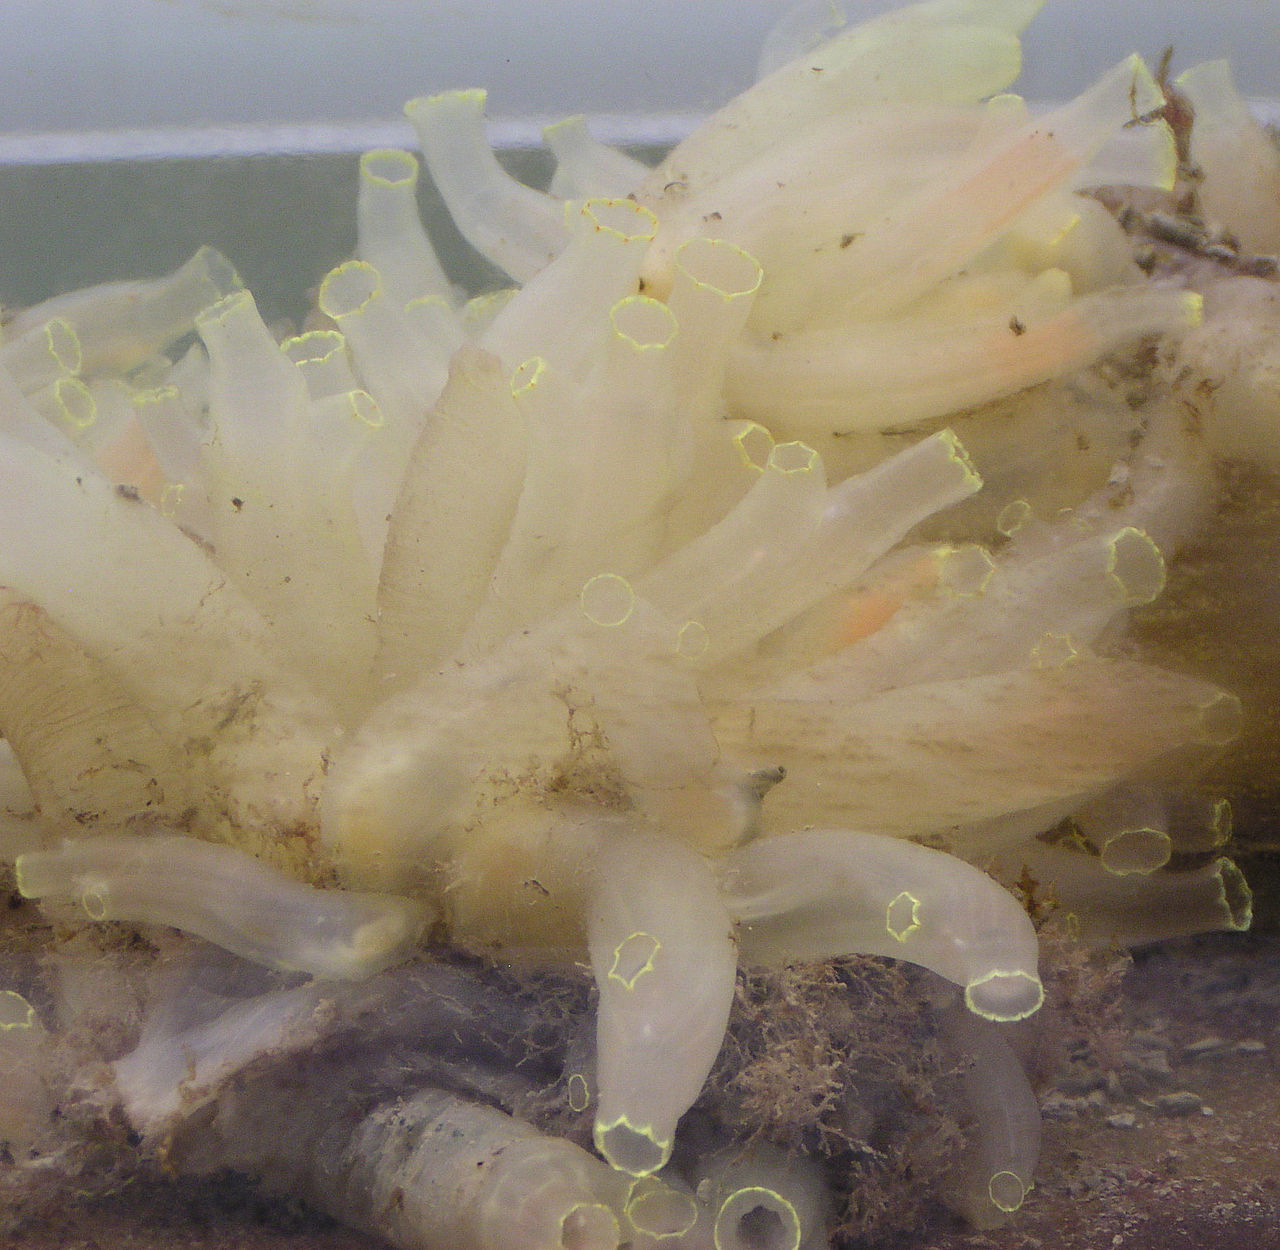
\includegraphics[scale=0.1]{illustrations/ciona.jpg}
\subfigure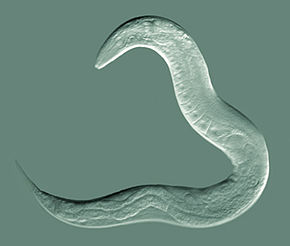
\includegraphics[scale=0.5]{illustrations/celegans.jpg}
\end{figure}

I thus implemented an interactive application in order to perform these tasks, to which other datasets can easily be added. The code (in Shiny, a R framework) is available here:\\  %TODO lien vers le code

Packages: R\cite{baser}, shiny\cite{shinyr}, scater\cite{scaterr}, rPython\cite{rpythonr}, RColorBrewer\cite{rcolorbrewerr}, NMF\cite{nmfr}, MAST\cite{mastr}, ggplot2\cite{ggplot2r}, genefilter\cite{genefilterr}, gplots\cite{gplotsr}, calibrate\cite{calibrater}, shinyBS\cite{shinybsr}, shinythemes\cite{shinythemesr}, shinydashboard\cite{shinydashboardr}, shinyjs\cite{shinyjsr}, DT\cite{dtr}, shinycssloaders\cite{shinycssloadersr}, shinyDND\cite{shinydndr}, ggfortify\cite{ggfortifyr}, ggbiplot\cite{ggbiplotr}, plotrix\cite{plotrixr} and shinyWidgets\cite{shinywidgetsr}.\\

\section{Objectives}

After obtaining the gene expression matrix, one may be interested in knowing the number of subpopulations of cells, that is, of groups of similar cells, but also which genes are expressed differently from one cell group to another (\textbf{differential expression analysis}), or visualizing the whole cell population in the observed data (see Figure \ref{pipeline}). One may also would like to know the \textbf{gene expression pattern} for each feature, that is, the sets of most expressed and less highly expressed genes in the cell.\\

There is already an application, called SAKE\cite{sake}, performing clustering (with Non-negative Matrix Factorization, see below for a description) and differential expression analysis. It is a really complete and interesting application. However, there are a lot of options, thus making the application not really intuitive, and does not display the gene expression patterns. Moreover, it uses DESeq2\cite{love2014moderated} to perform differential expression analysis, which is only a slightly modified version of a differential expression analyzer\cite{anders2010differential} for bulk RNA seq data, thus not taking into account some characteristics of sRNAseq data, such as the expected high number of null gene expression values (DESeq2 models gene expression as only following a negative binomial distribution, which is the one bulk RNAseq is assumed to follow).

\begin{figure}[H]
\centering
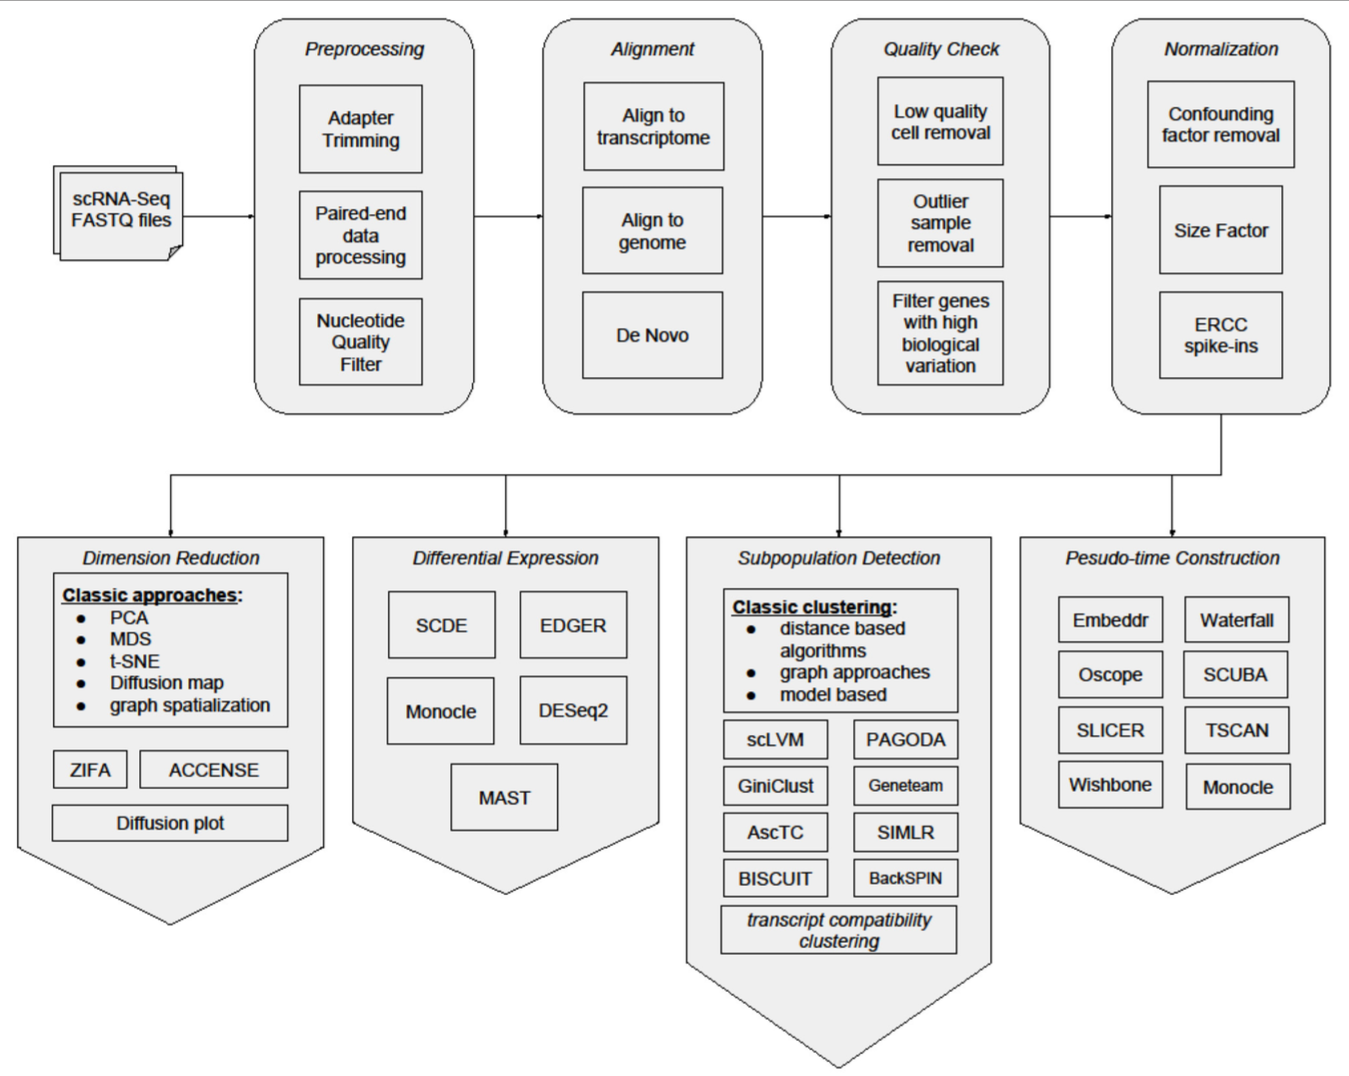
\includegraphics[scale=0.3]{illustrations/pipelinedownstream.png}
\caption{Possible downstream analysis pipeline after alignment and quality check of the resulting gene expression matrix\cite{poirion2016single}}
\label{pipeline}
\end{figure}

\section{Implementation}

This is an example about how to use the application with the \textit{Ciona intestinalis} dataset\cite{suyama2016singlecell} (the dataset can be modified using the button on the top left of the application front page). I will compare the results obtained with the application (for cell B5.2 against B5.1, A5.1, A5.2, a5.3, a5.4 and b5.3, b5.4, and genes KH.C9.853 and KH.C13.27) and Figure D, page 382, in \cite{matsuoka2013transcriptome}.\\

In the \textbf{Data visualization} tab (see Figure \ref{menu}),  the front page displays a Principal Component Analysis (PCA) plot, indicating each cell type and embryo by a certain shape and colour, which is meant to give a visualization of all cells in the dataset, and help selecting the relevant cell groups.\\

On the right side, the heatmap is coloured according to the number of raw counts in each cell for each of the $min(10, p)$ most highly-expressed genes (where $p$ is the number of genes), in order to visualize the potentially gene outliers\cite{poirion2016single}. On the sides can be seen hierarchical clusterings of the cells (on top), and of the genes (on the left).\\

The two groups (or conditions) to compare can be selected by drag and drop (see Figure \ref{cellselection}).\\

\begin{figure}[H]
\centering
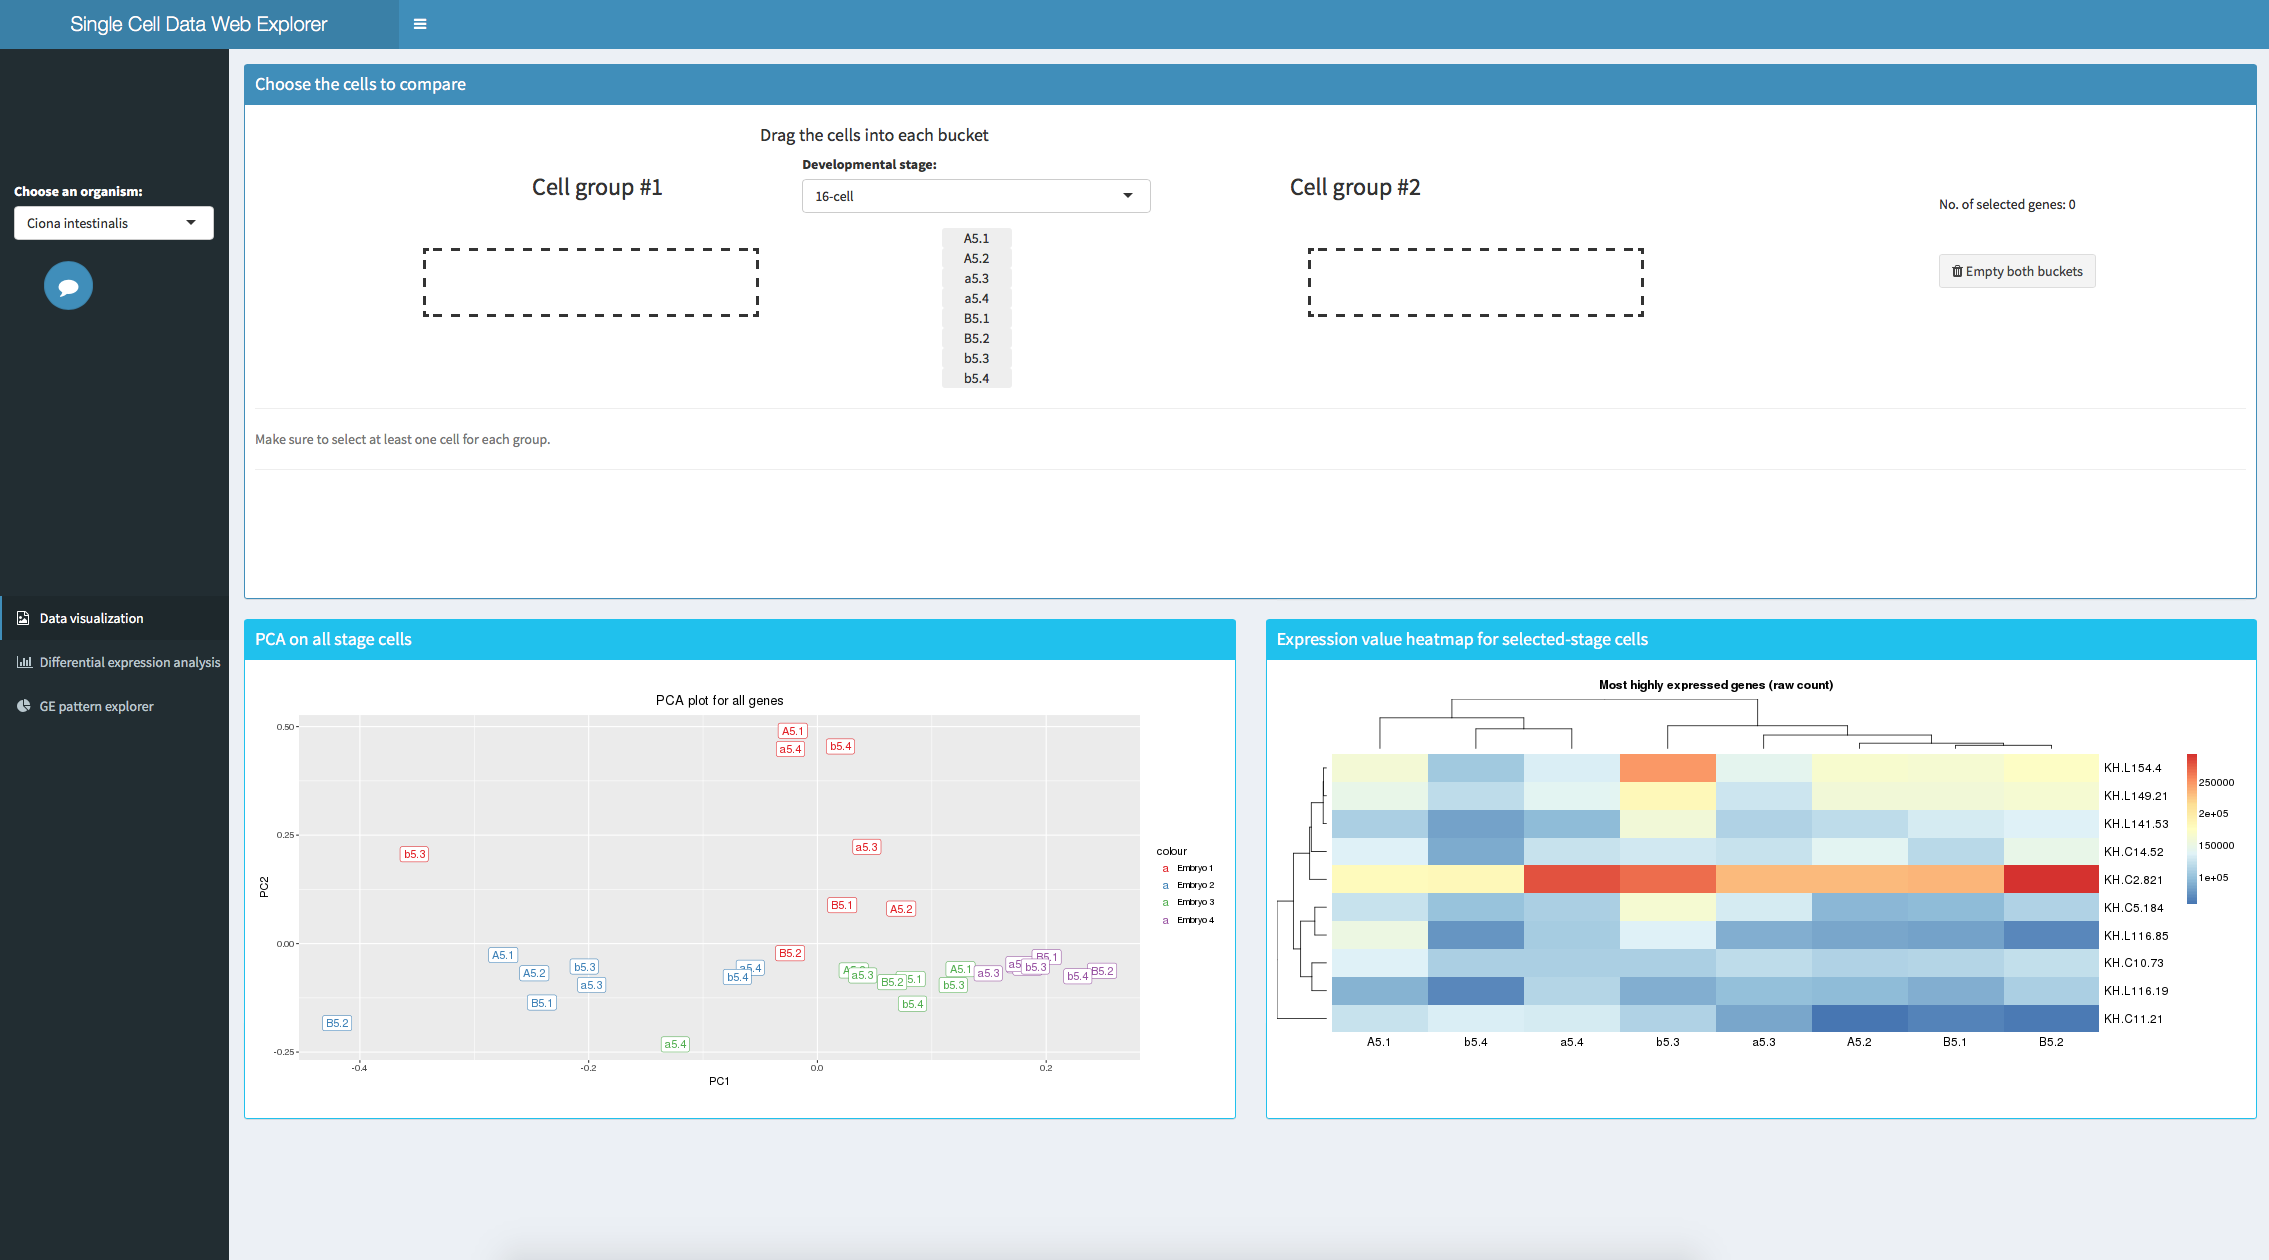
\includegraphics[scale=0.2]{application/menu.png}
\caption{Menu}
\label{menu}
\end{figure}

\begin{figure}[H]
\centering
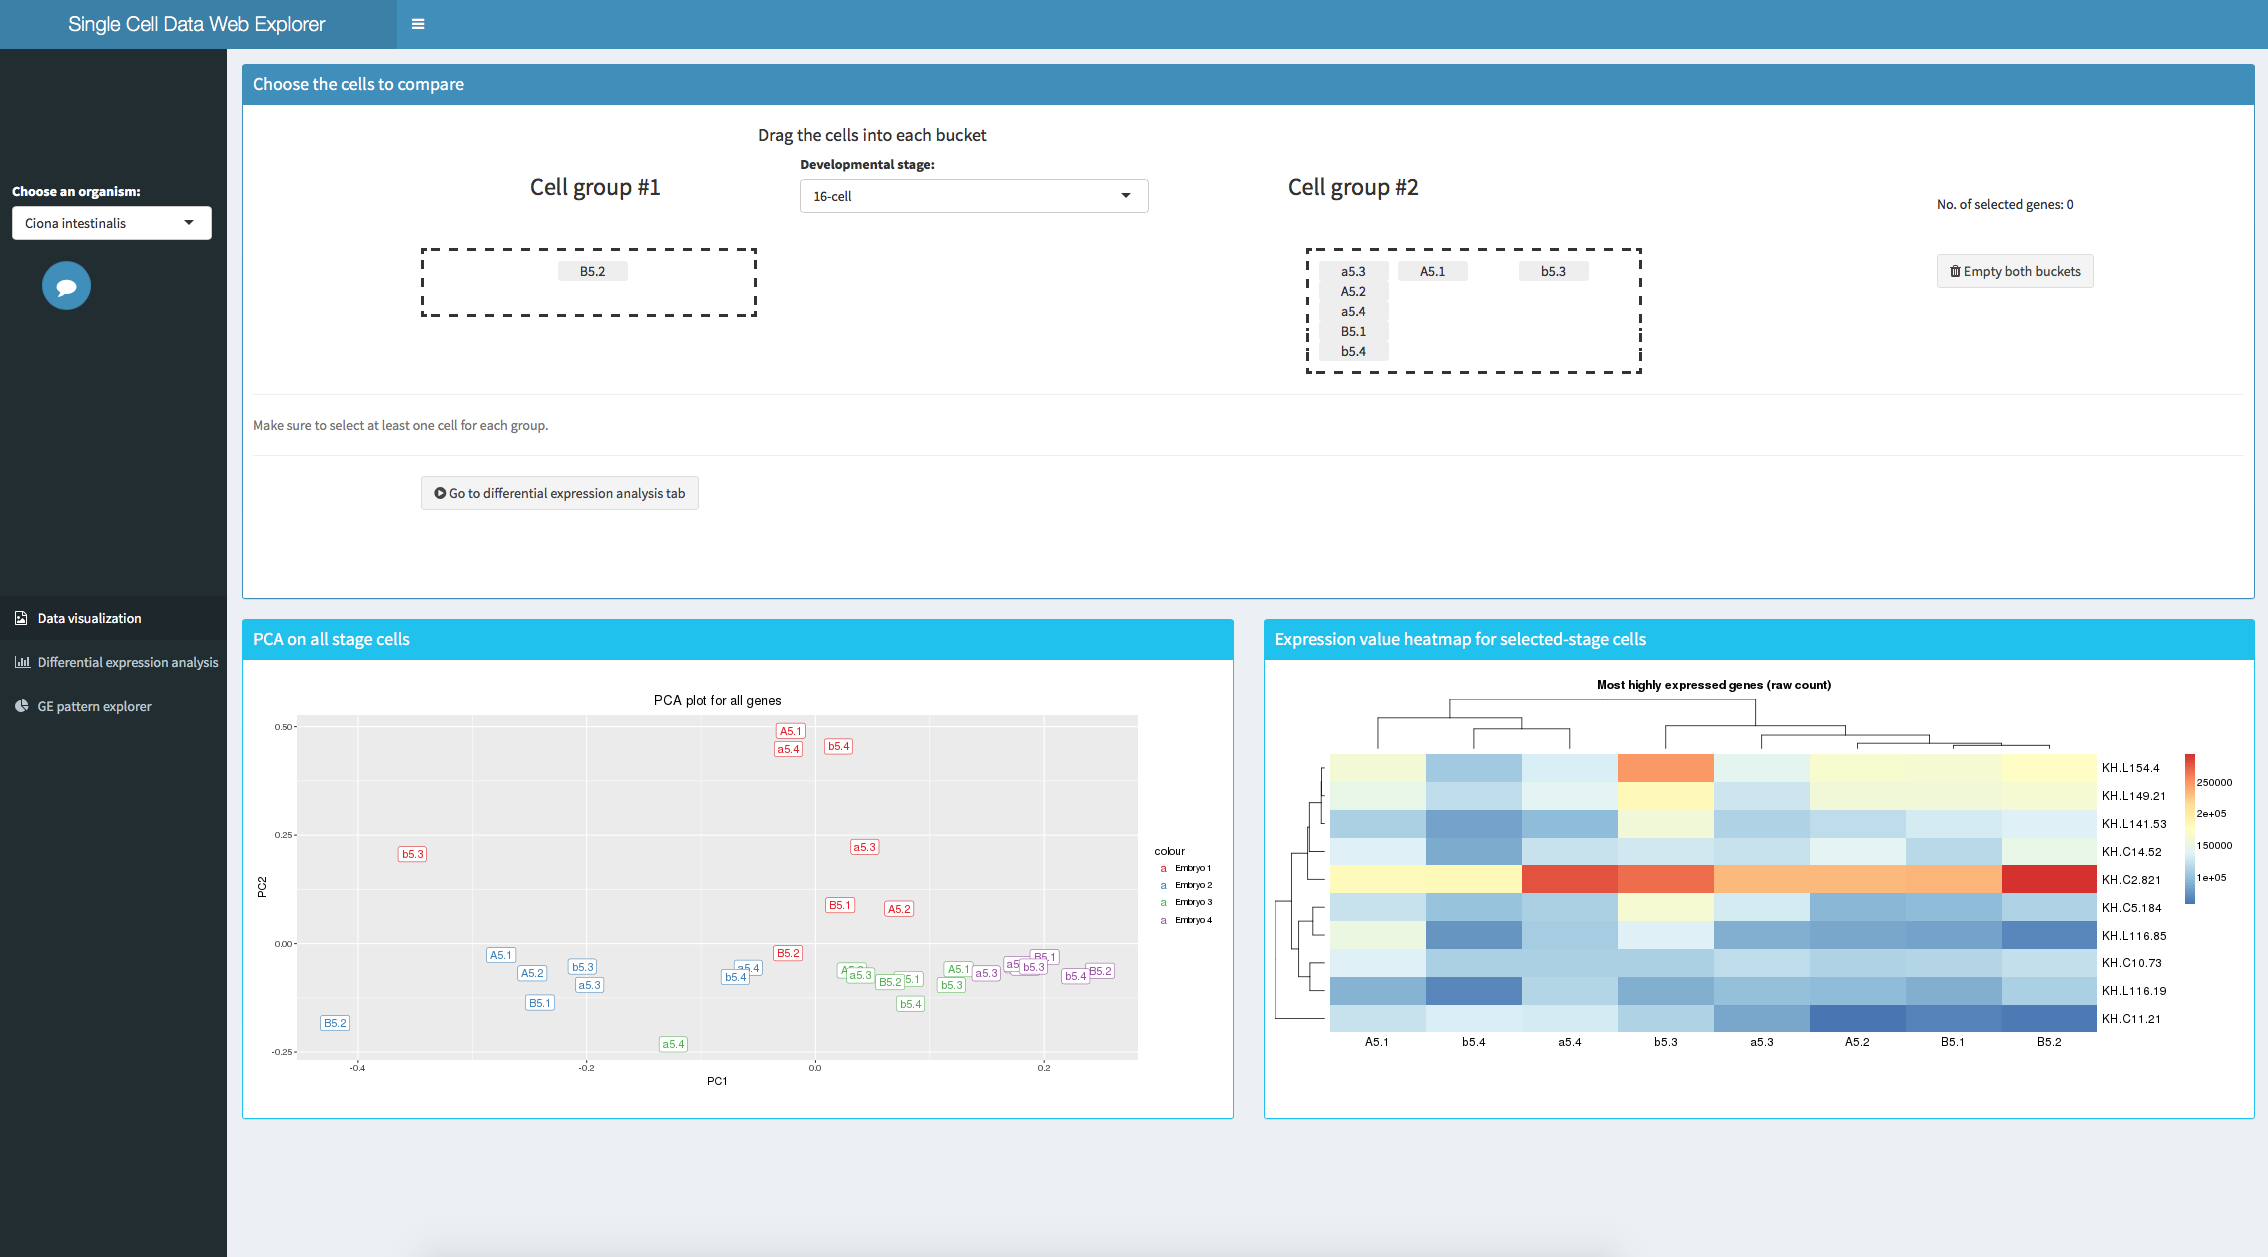
\includegraphics[scale=0.2]{application/cellselection.png}
\caption{Cell group selection}
\label{cellselection}
\end{figure}

At first, the \textbf{Differential expression analysis} tab (see Figure \ref{geneselection}) allows the user to view the raw counts of every gene in every cell of the dataset. Then genes can be selected directly from the table (or using the provided buttons). The user can search for a given gene with the search bar on the top-right corner of the table. The PCA biplot can be updated: the PCA is then performed on the currently selected genes.\\

\begin{figure}[H]
\centering
\subfigure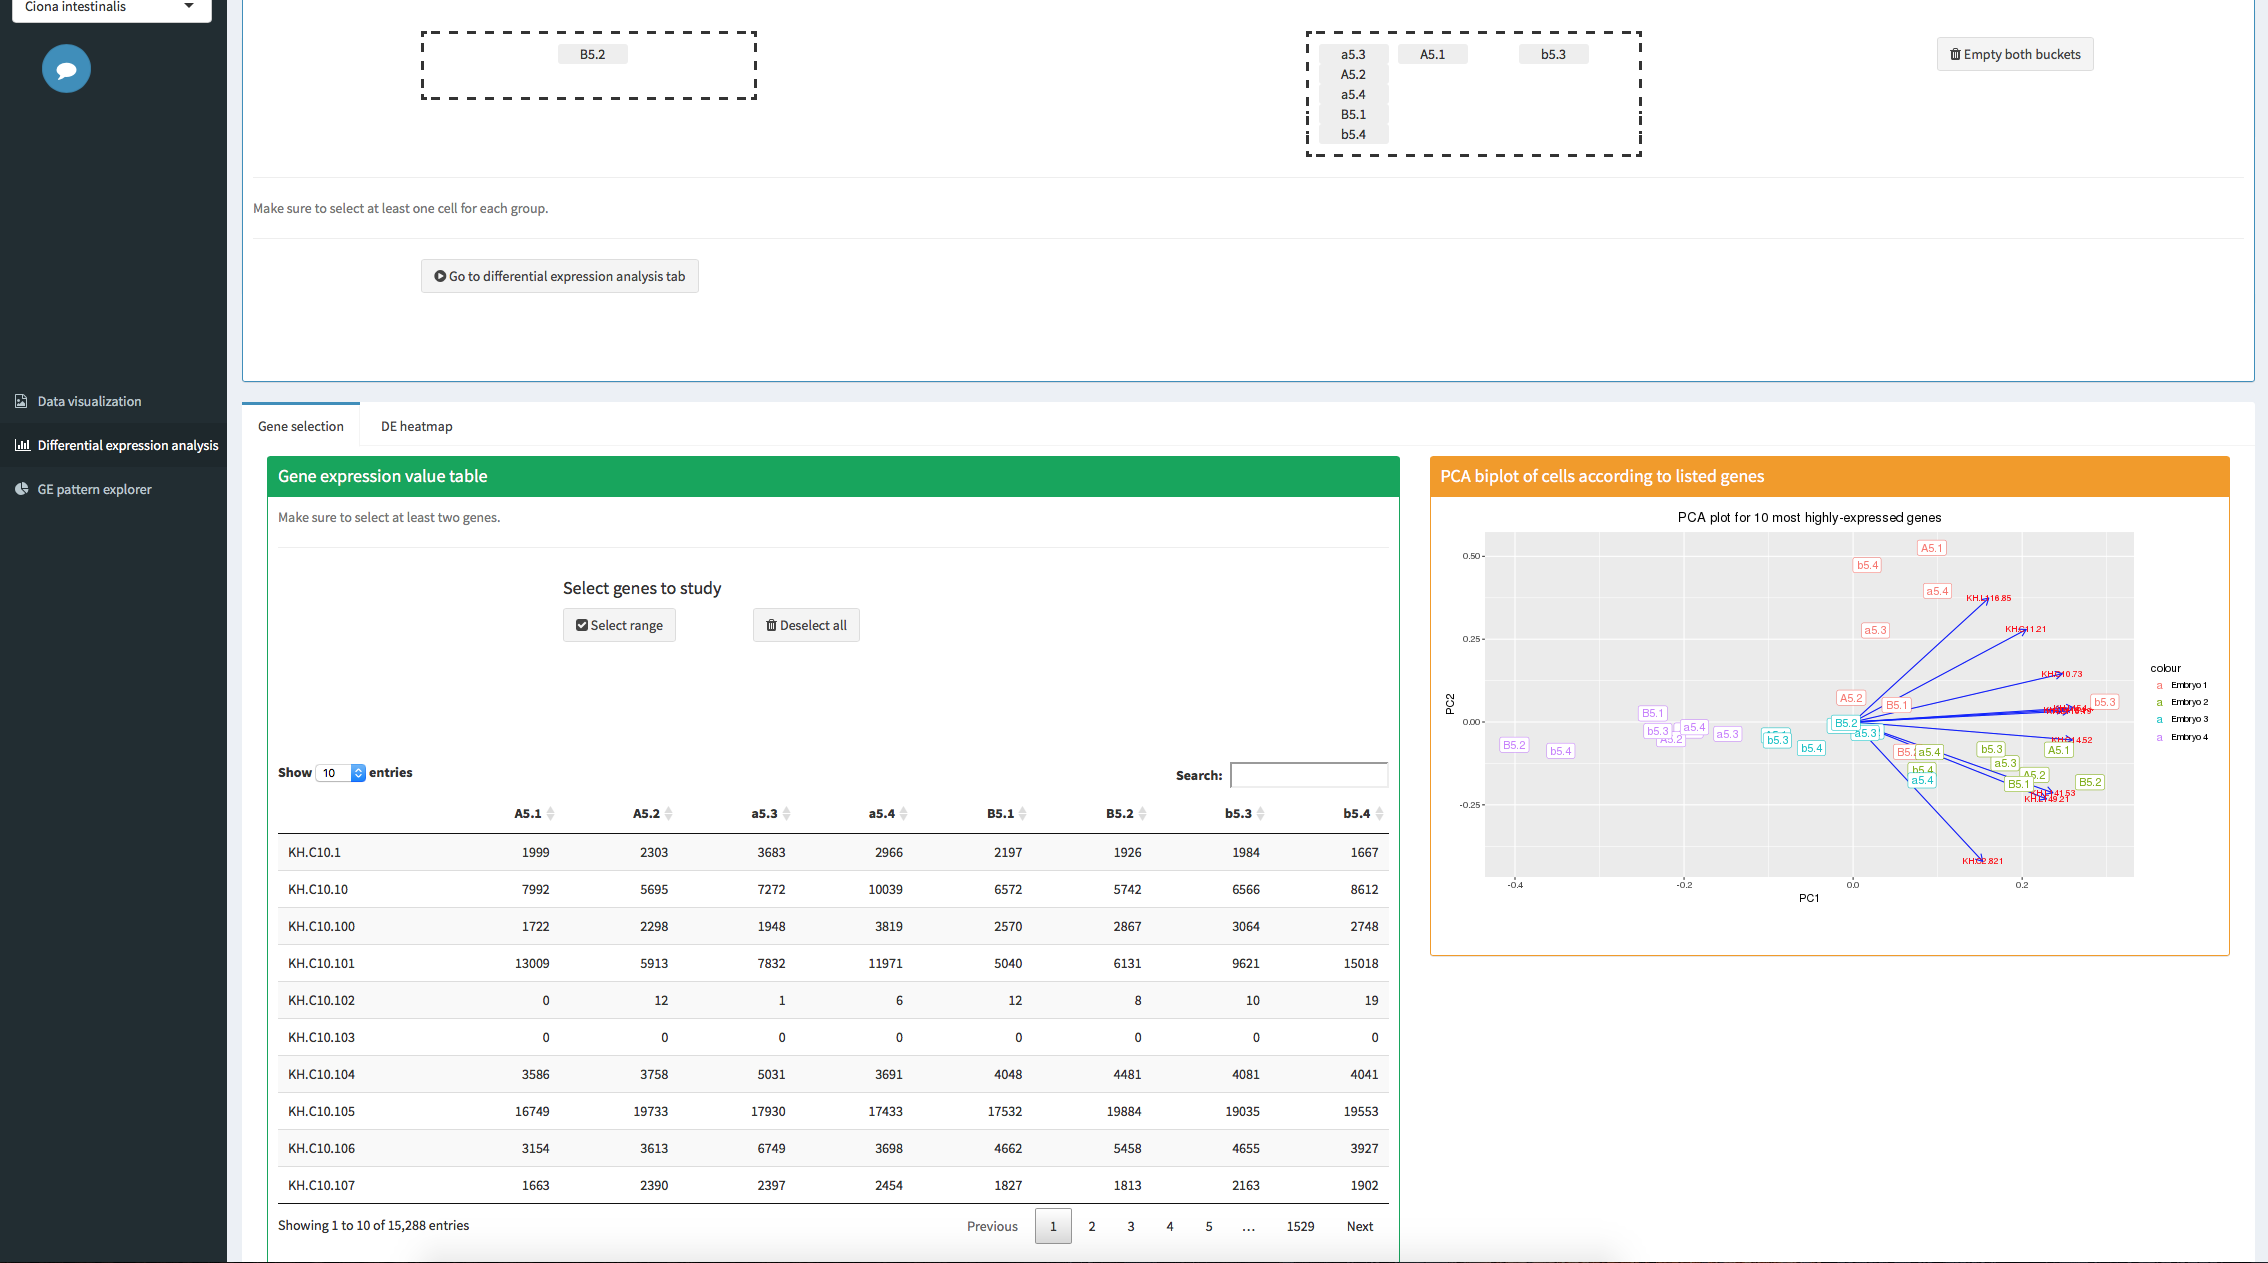
\includegraphics[scale=0.2]{application/geneselection.png}
\subfigure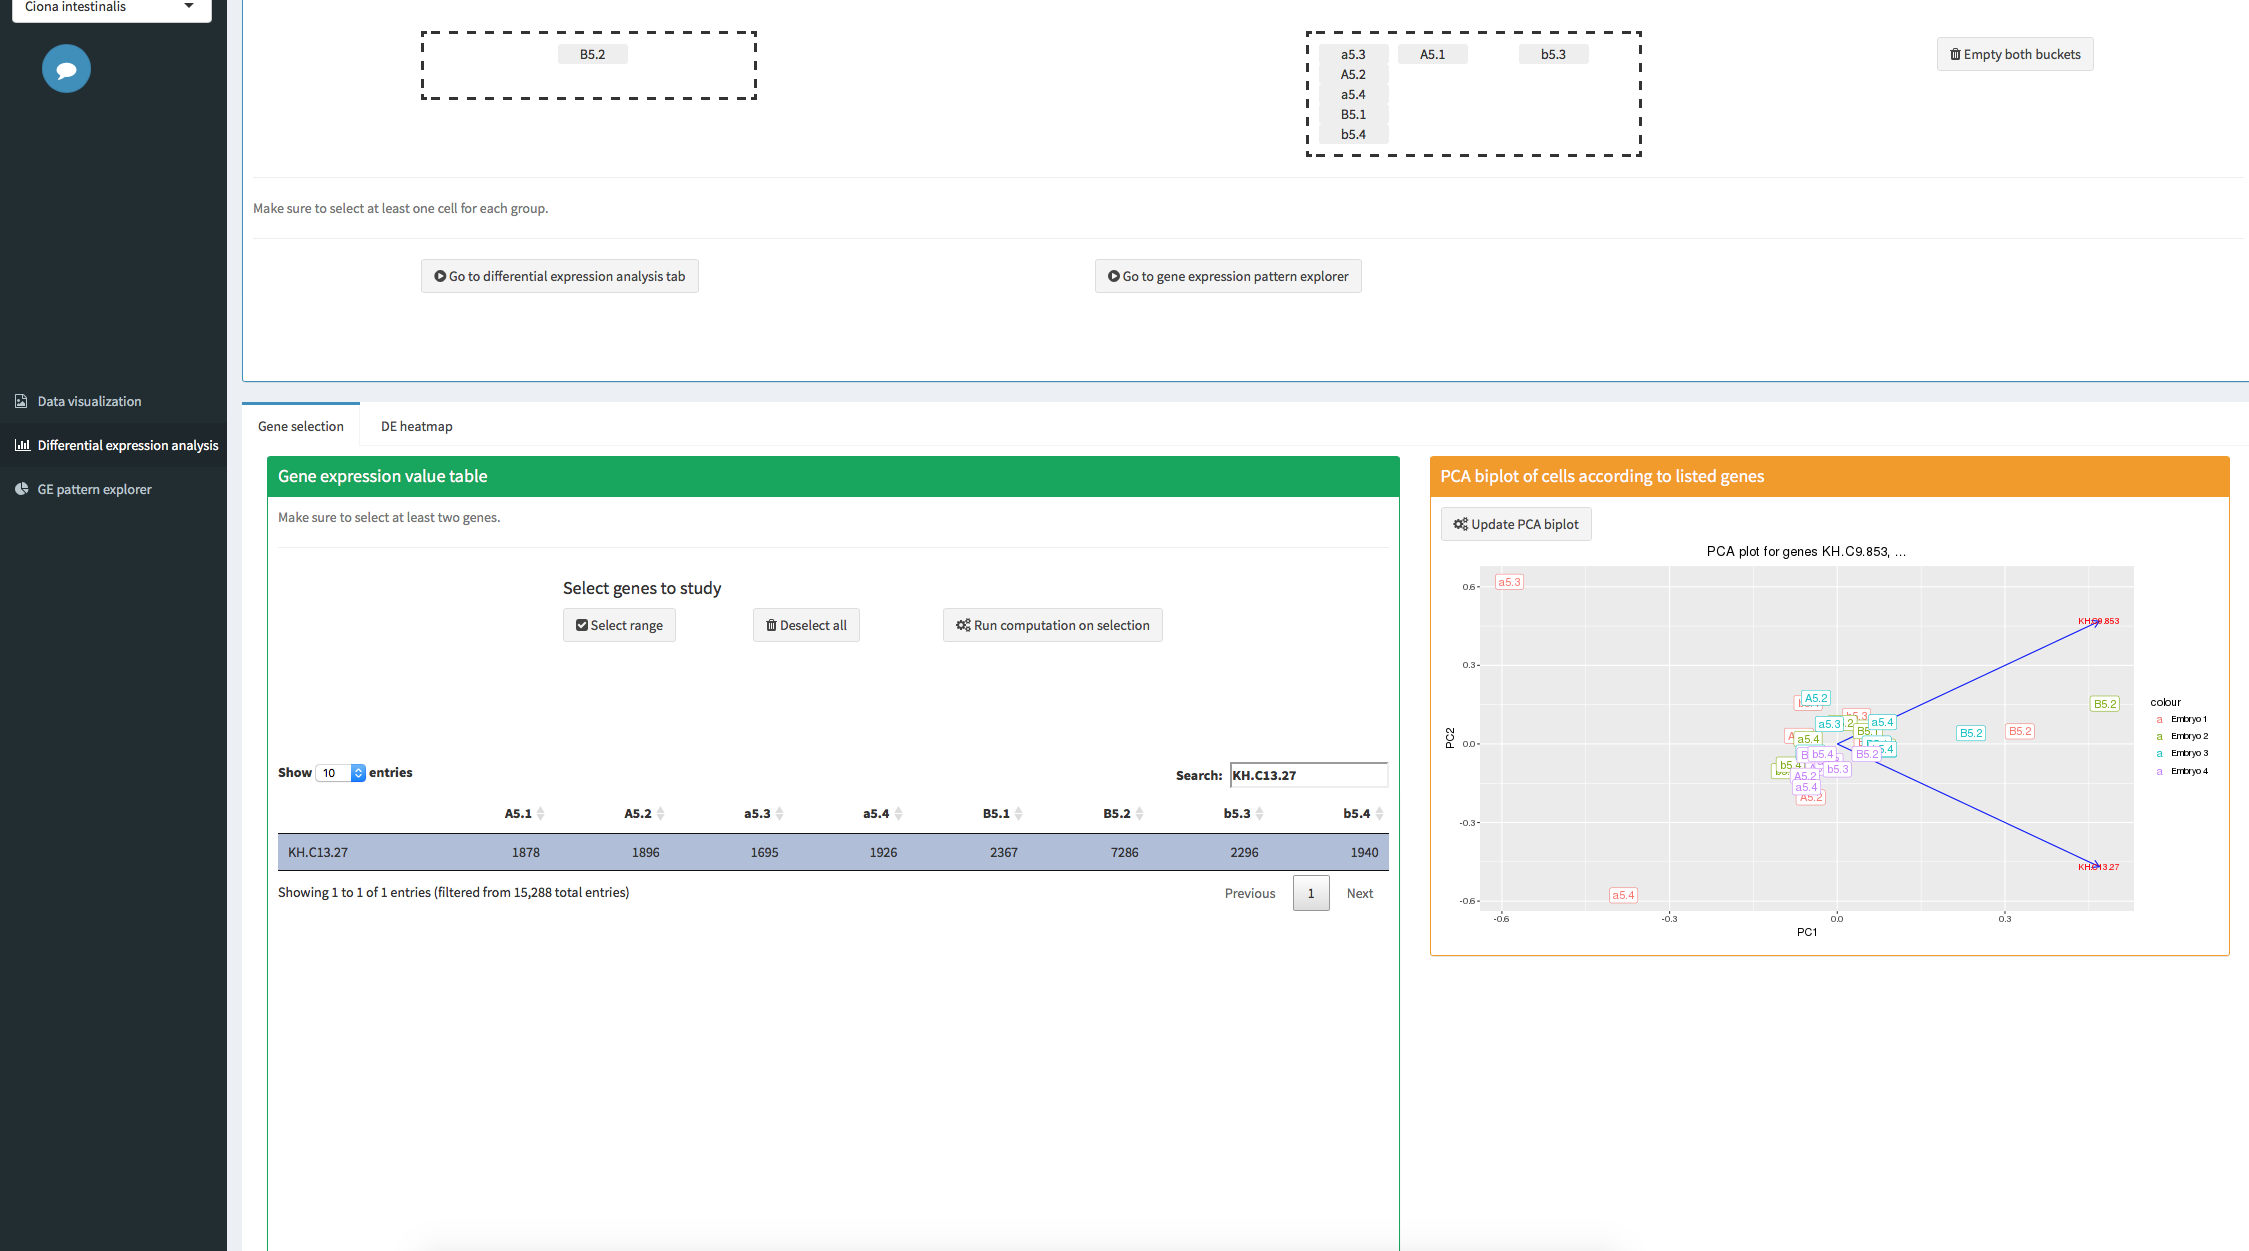
\includegraphics[scale=0.2]{application/geneselected.png}
\caption{Gene selection panel}
\label{geneselection}
\end{figure}

Differential expression analysis pipeline (from MAST package\cite{finak2015mast}) is performed on the selected genes and cell groups when clicking on "Run computation on selection" button (see Figure \ref{geneselection}). After a few seconds of computing, the front page displays the table with genes ranked in increasing \textbf{p-value} order (see Figure \ref{de}). The p-values are a way to quantify the probability that a certain gene can be differentially expressed \textit{only by chance} between the two cell groups: the lower a p-value is, the more the associated gene is likely to be differentially expressed in practice.\\

In the other tab, there is a heatmap with the selected cells and the most \textbf{differentially-expressed genes} (the genes which expression level strongly differs according to the considered cell group), with associated hierarchical clusterings (on genes on the left, on cells on top of the heatmap (see Figure \ref{de}).\\

Moreoever, the application offers now the opportunity to select genes according to their \textbf{p-values}. The cutoff value is user-selected with the slider bar (see Figures \ref{pcutoff}).\\

\begin{figure}[H]
\centering
\subfigure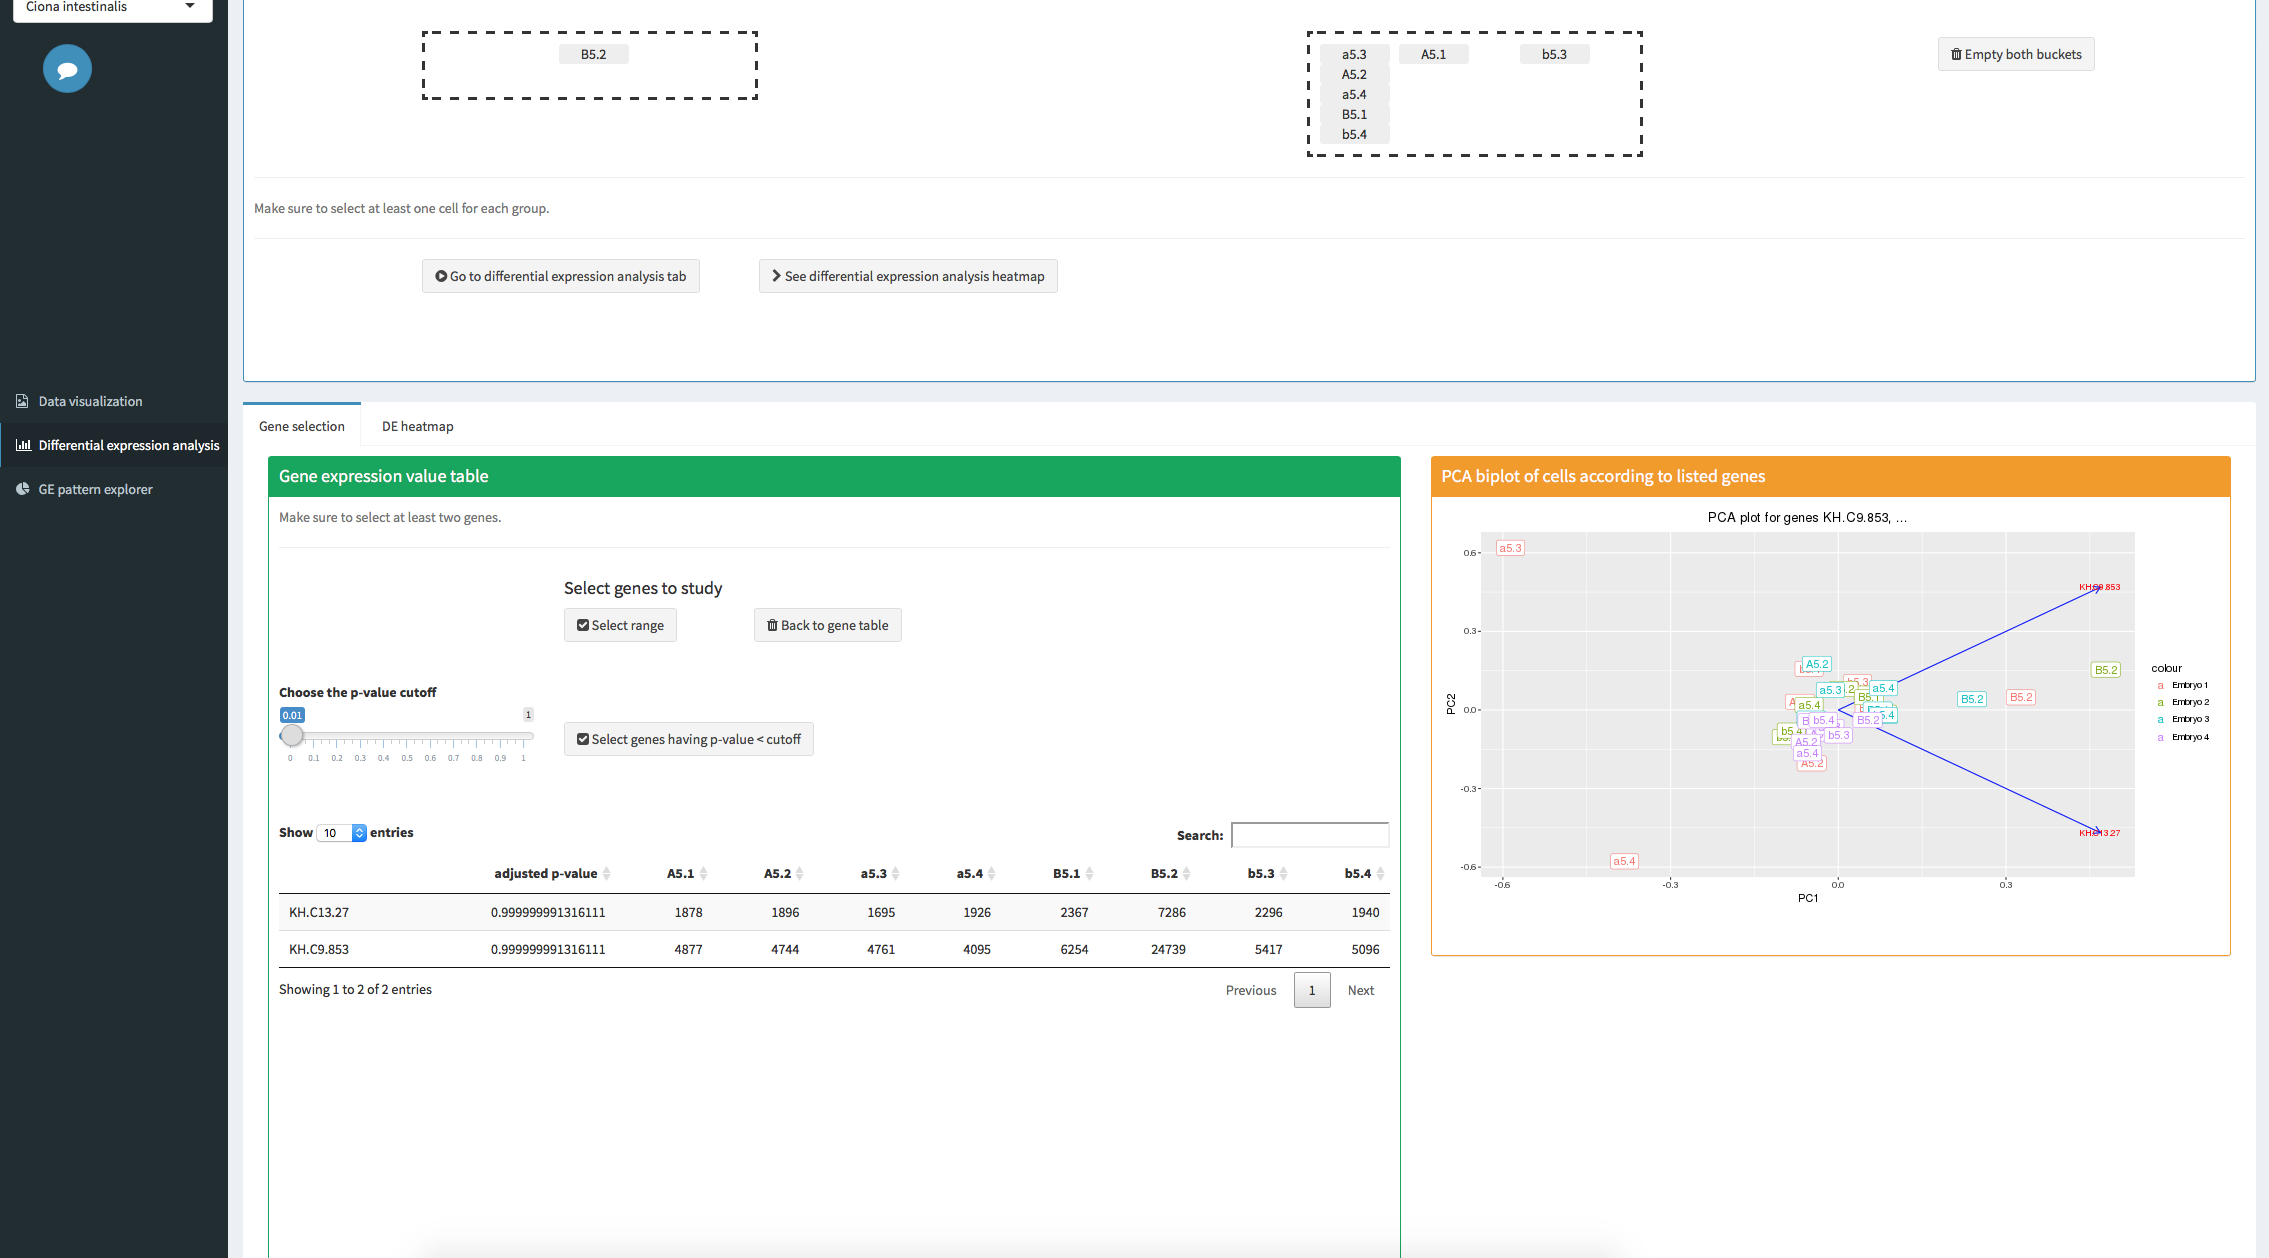
\includegraphics[scale=0.2]{application/pvalue-results.png}
\subfigure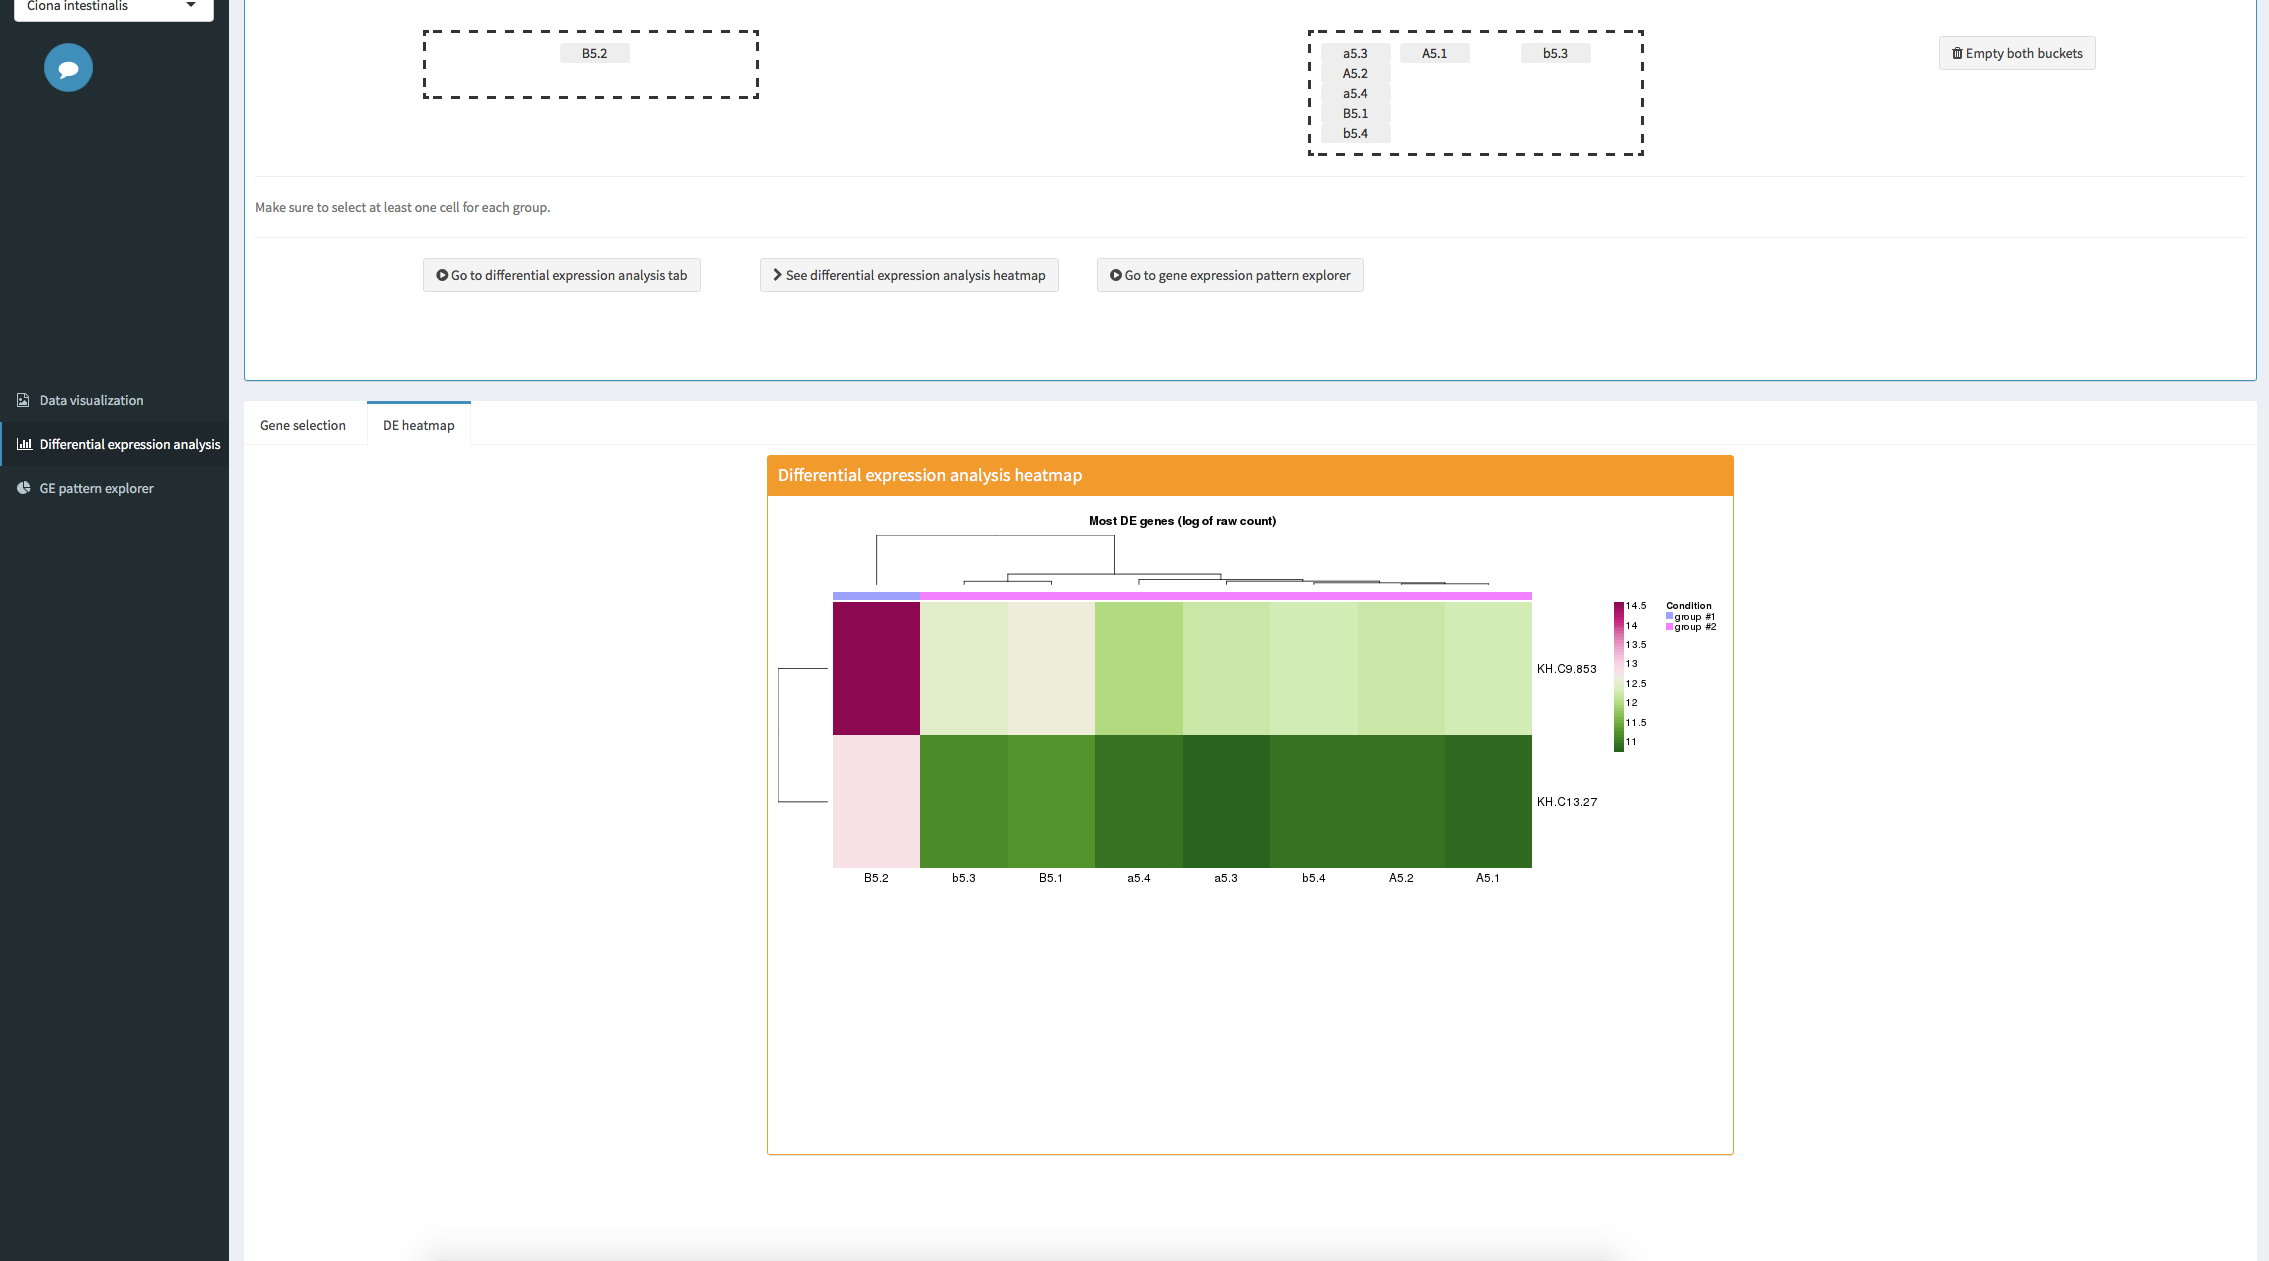
\includegraphics[scale=0.2]{application/de-results.png}
\caption{Differential expression analysis results}
\label{de}
\end{figure}

\begin{figure}[H]
\centering
\subfigure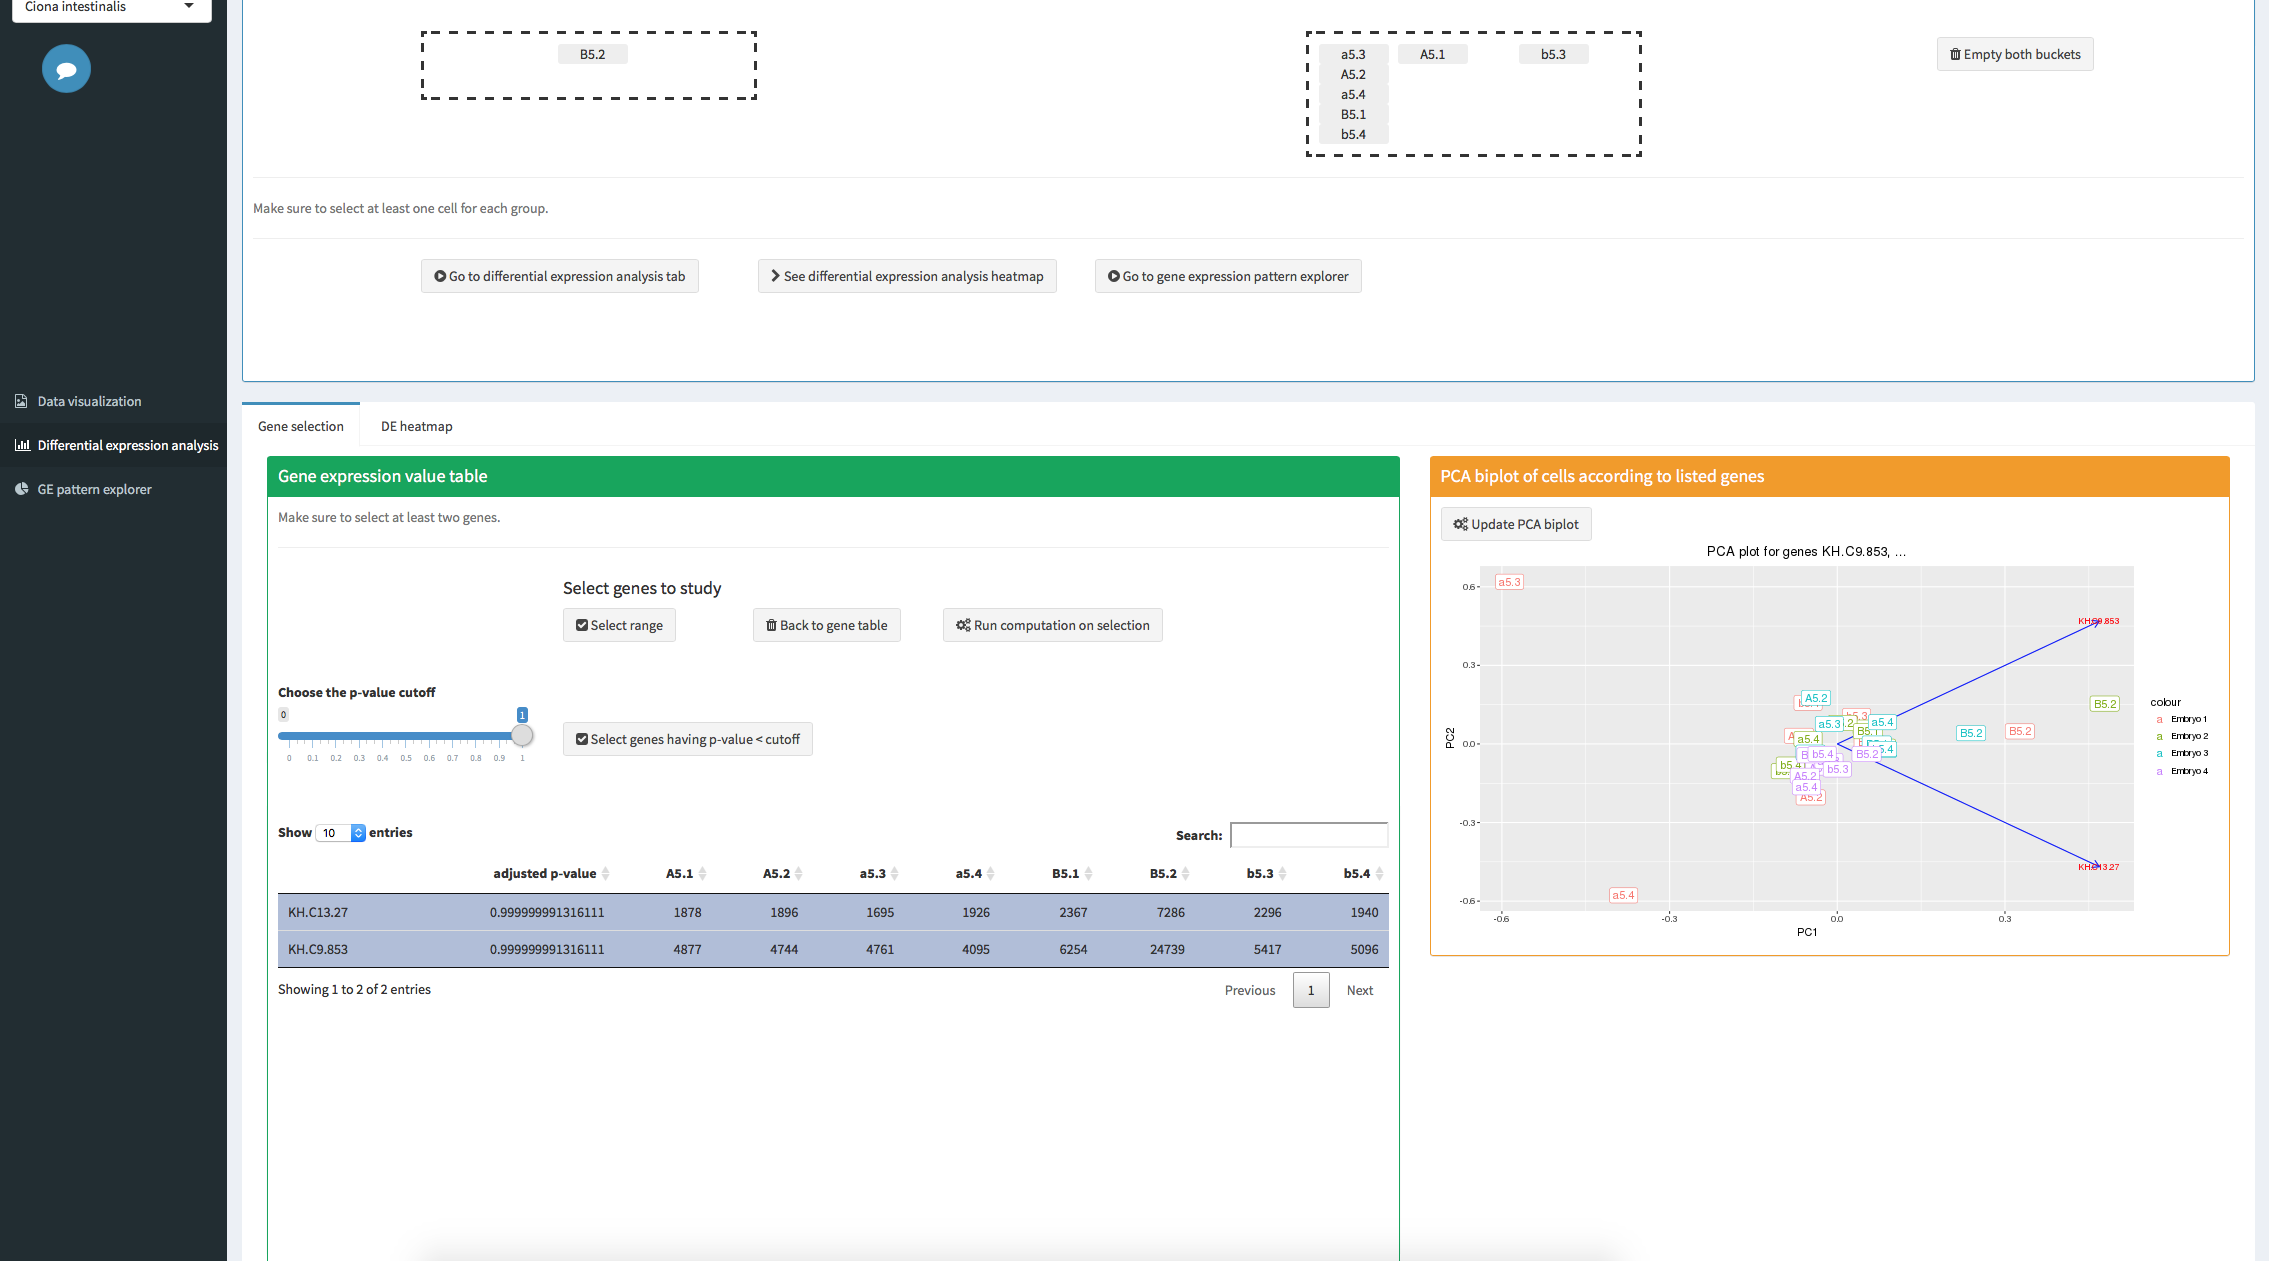
\includegraphics[scale=0.2]{application/selectpvaluecutoff.png}
\subfigure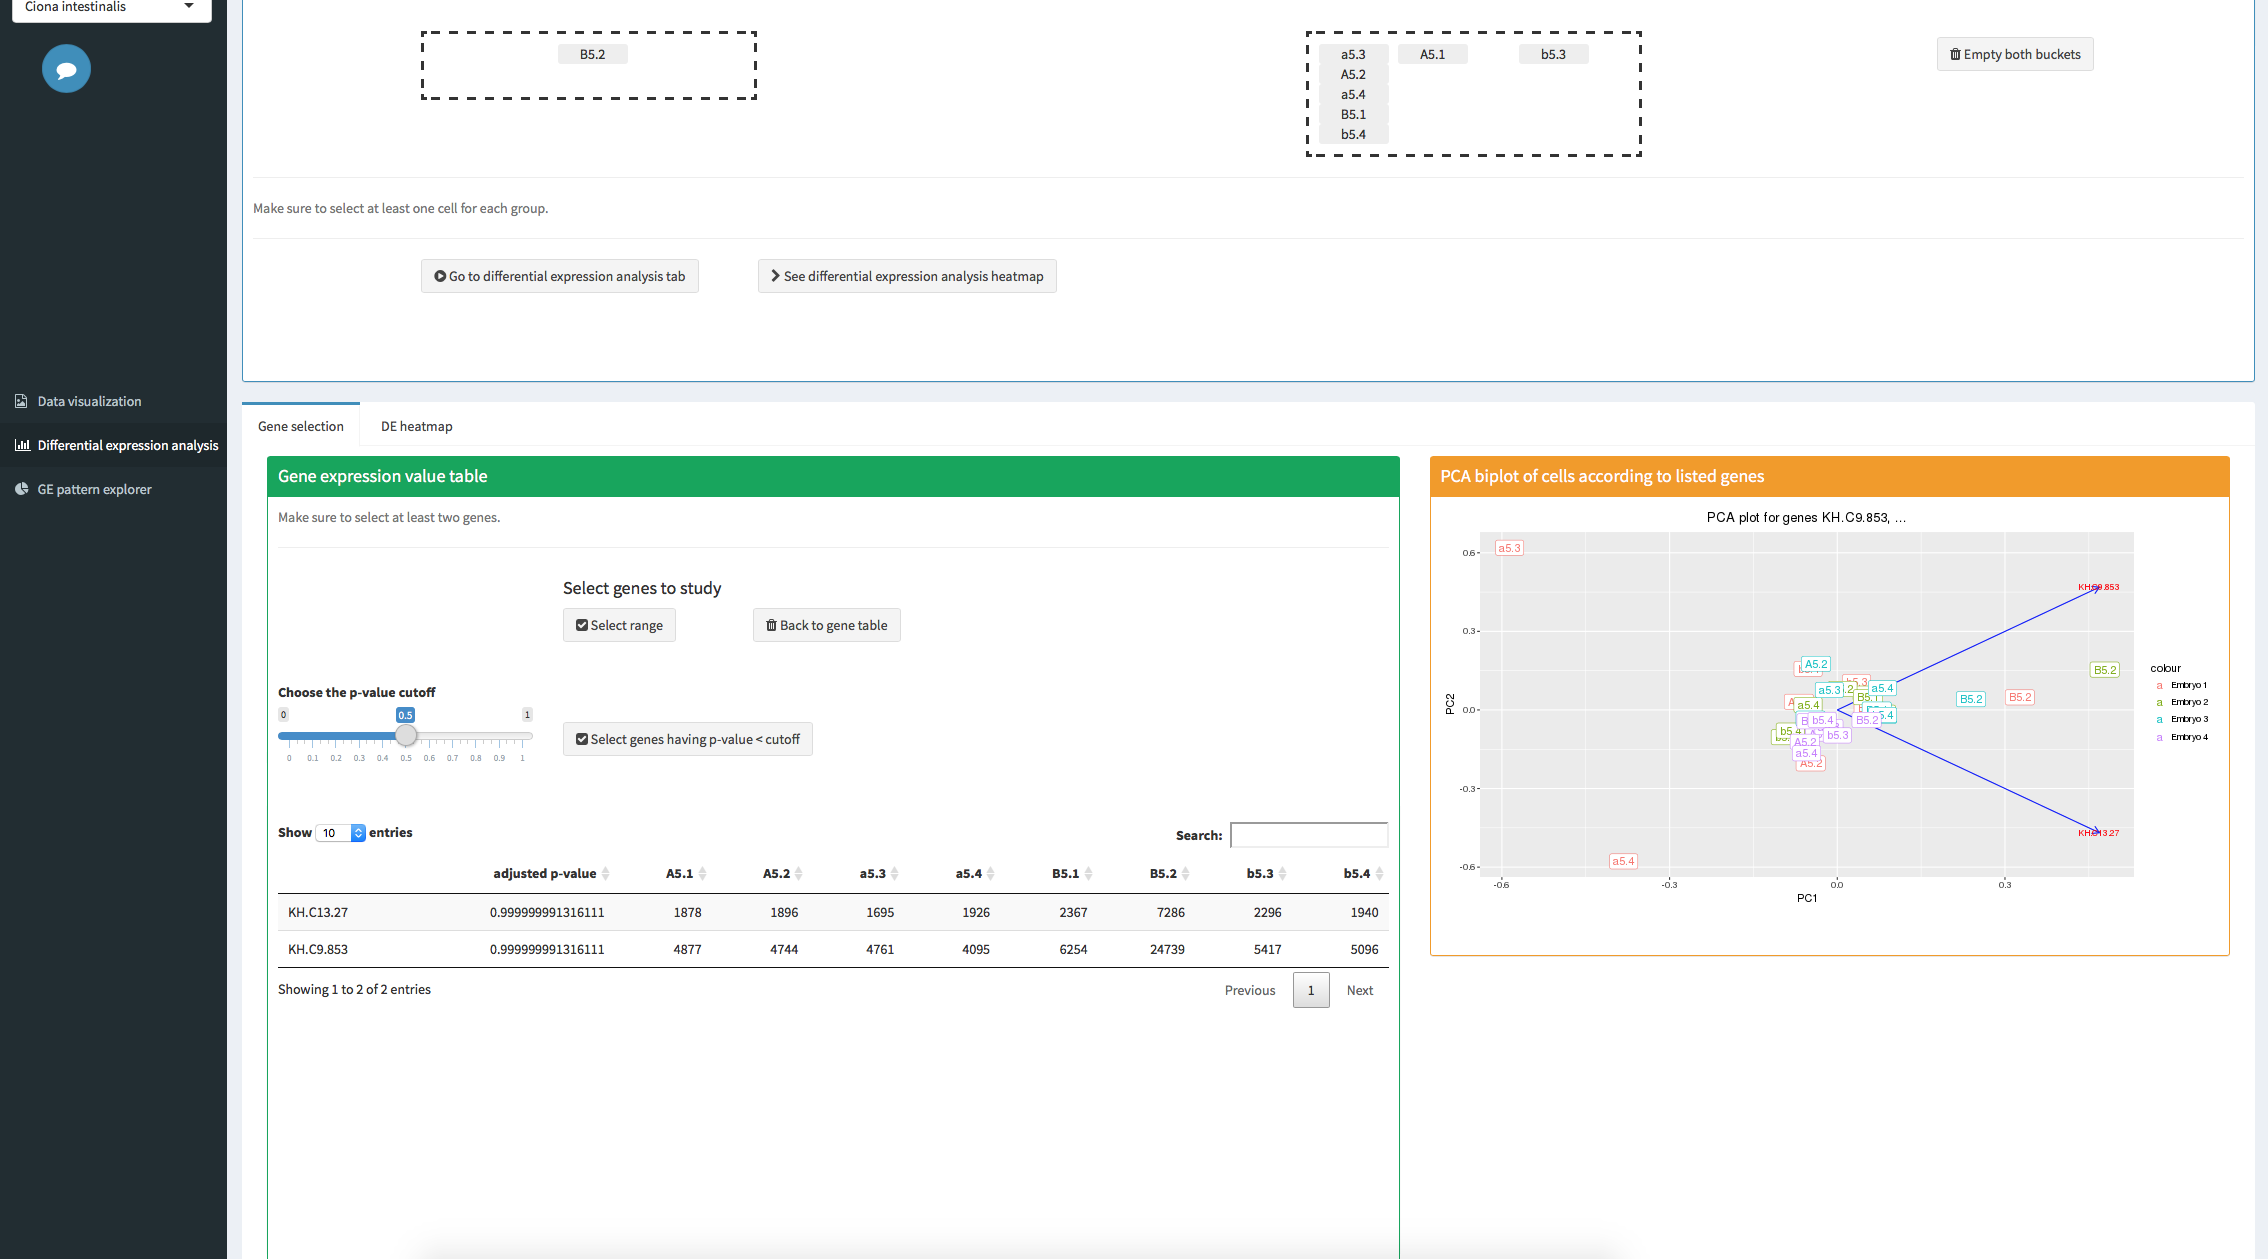
\includegraphics[scale=0.2]{application/selectpvaluecutoff2.png}
\caption{Gene selection with p-value cutoff}
\label{pcutoff}
\end{figure}

In the \textbf{Gene expression pattern visualization} tab (see Figure \ref{visualization}), when the selected threshold type is set to "Binary", the front page displays a schema of the selected cells in each group, where each rectangle represents one of the selected genes.\\

Given the threshold value (in percentage of the total raw count expression value of a given gene in a given cell), the rectangle is colored if and only if the gene expression raw count value of the gene in the cell is over this threshold. For instance, if the threshold is fixed to 10\% of the total expression value, the rectangle associated with gene $i$ in the set of rectangles corresponding to cell $j$ will be colored if and only if (M being the gene expression matrix) $M_{i,j} > 10\% \times \sum{_{k}}{M_{k, j}}$. It should be kept in mind that cell gene patterns cannot be compared directly, since the expressiveness of a given gene is only determined by the ratio gene expression value/ total gene expression value in the considered cell.\\

The threshold value is user-selected with a slider bar (see Figure \ref{visualization}).\\

When the threshold type is set to "Graded", the gene expression patterns are colored according to the legend displayed on the left, the same way as with binary threshold (see Figure \ref{graded}).\\

Eventually, a script is also provided to make adding new datasets to the application easier. Source code and other tests can be found at: {\url{https://github.com/oist-gene-clustering/scwebexplorer}}

\begin{figure}[H]
\centering
\subfigure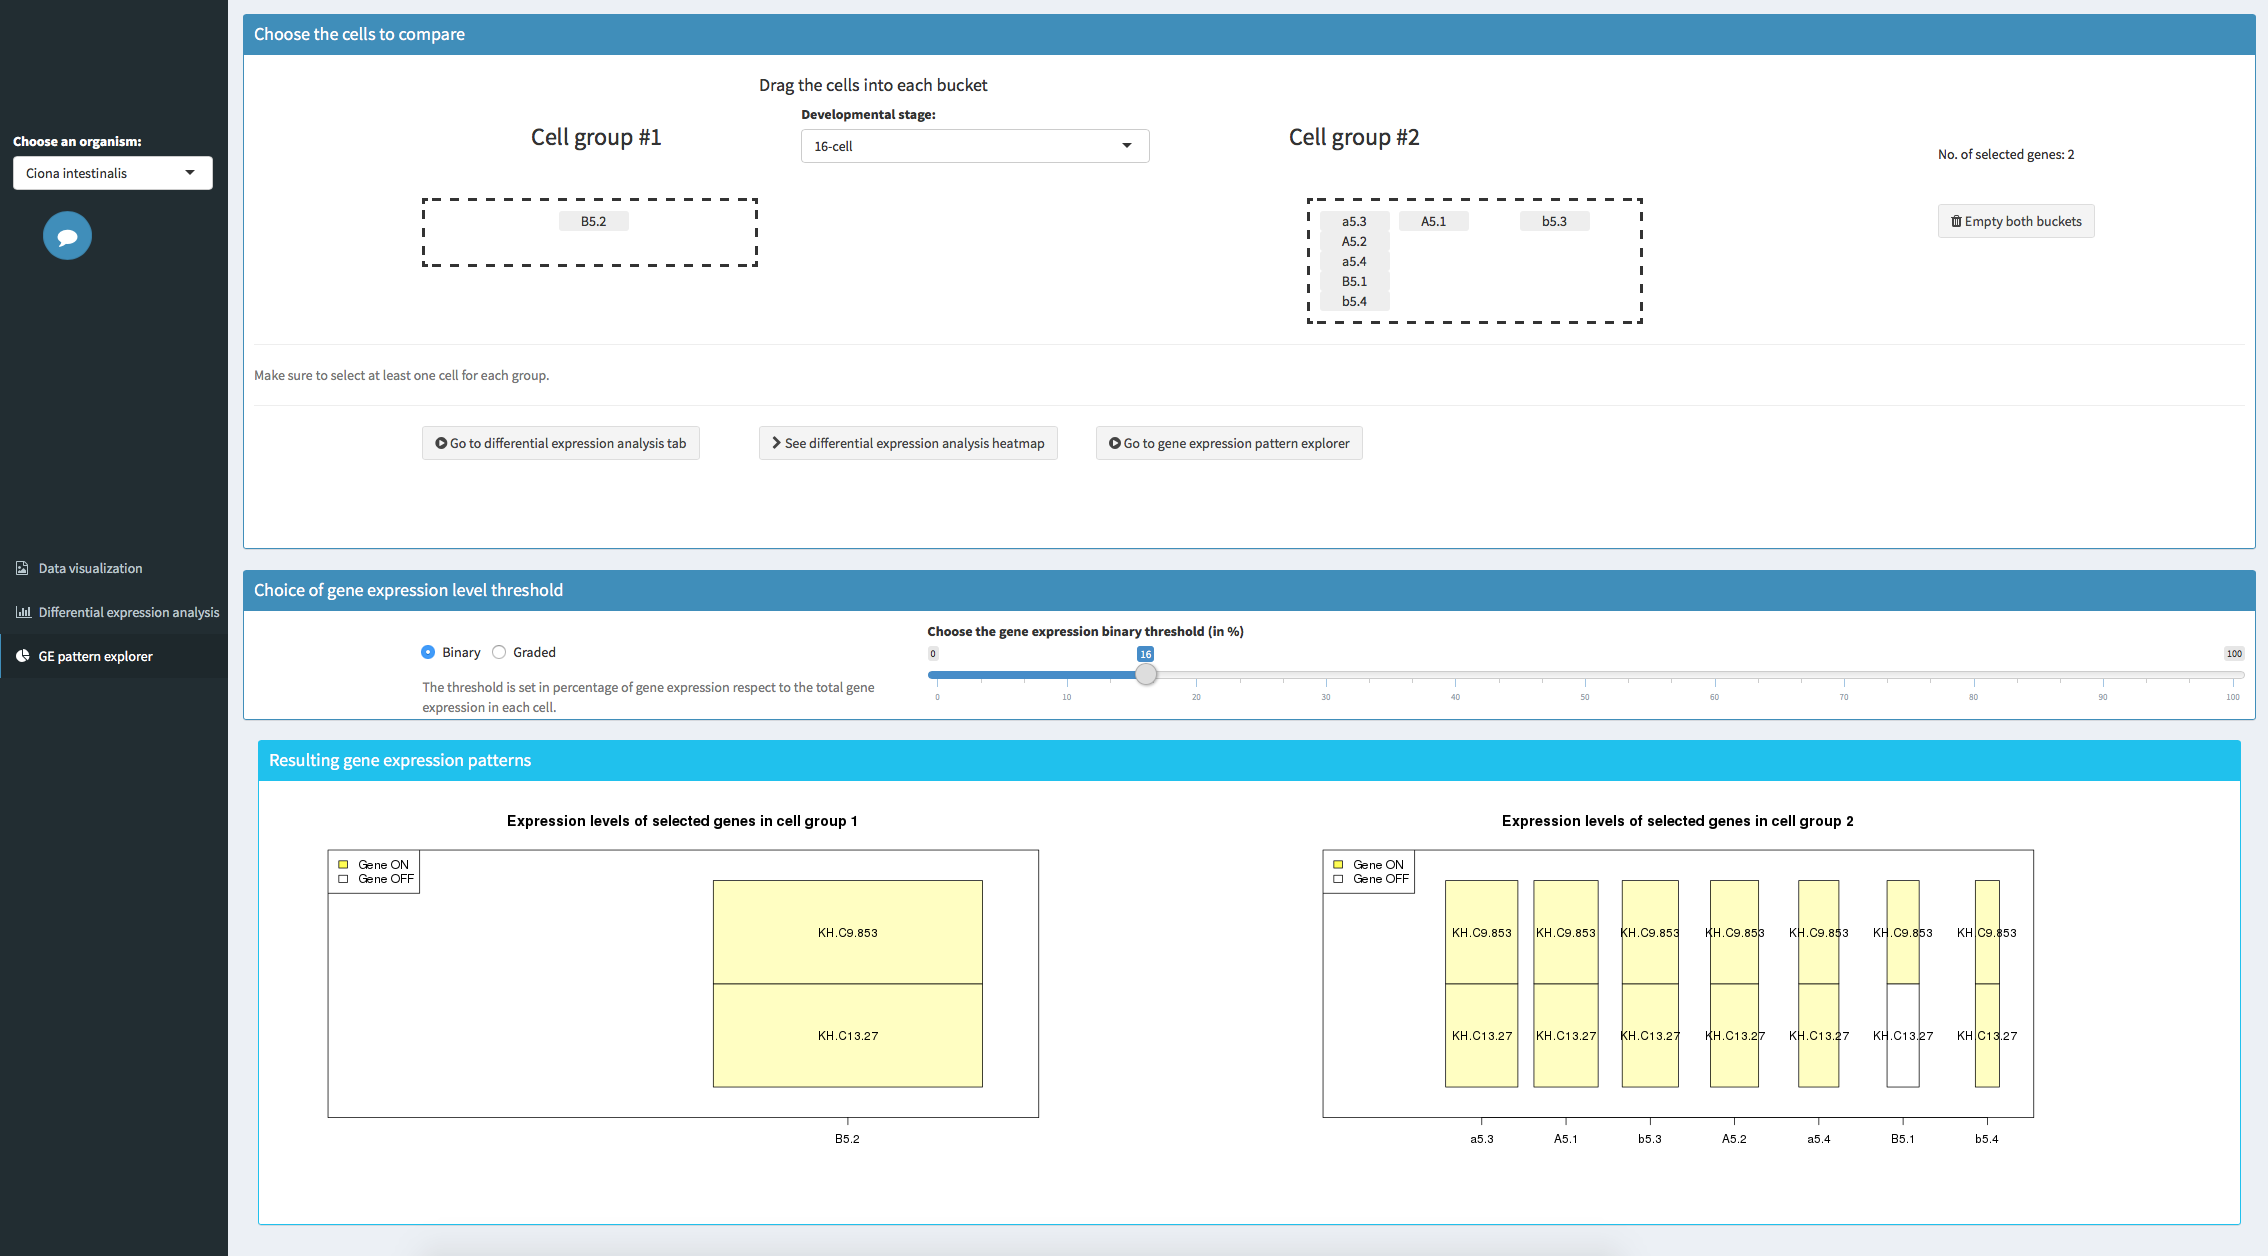
\includegraphics[scale=0.2]{application/patternthres1.png}
\subfigure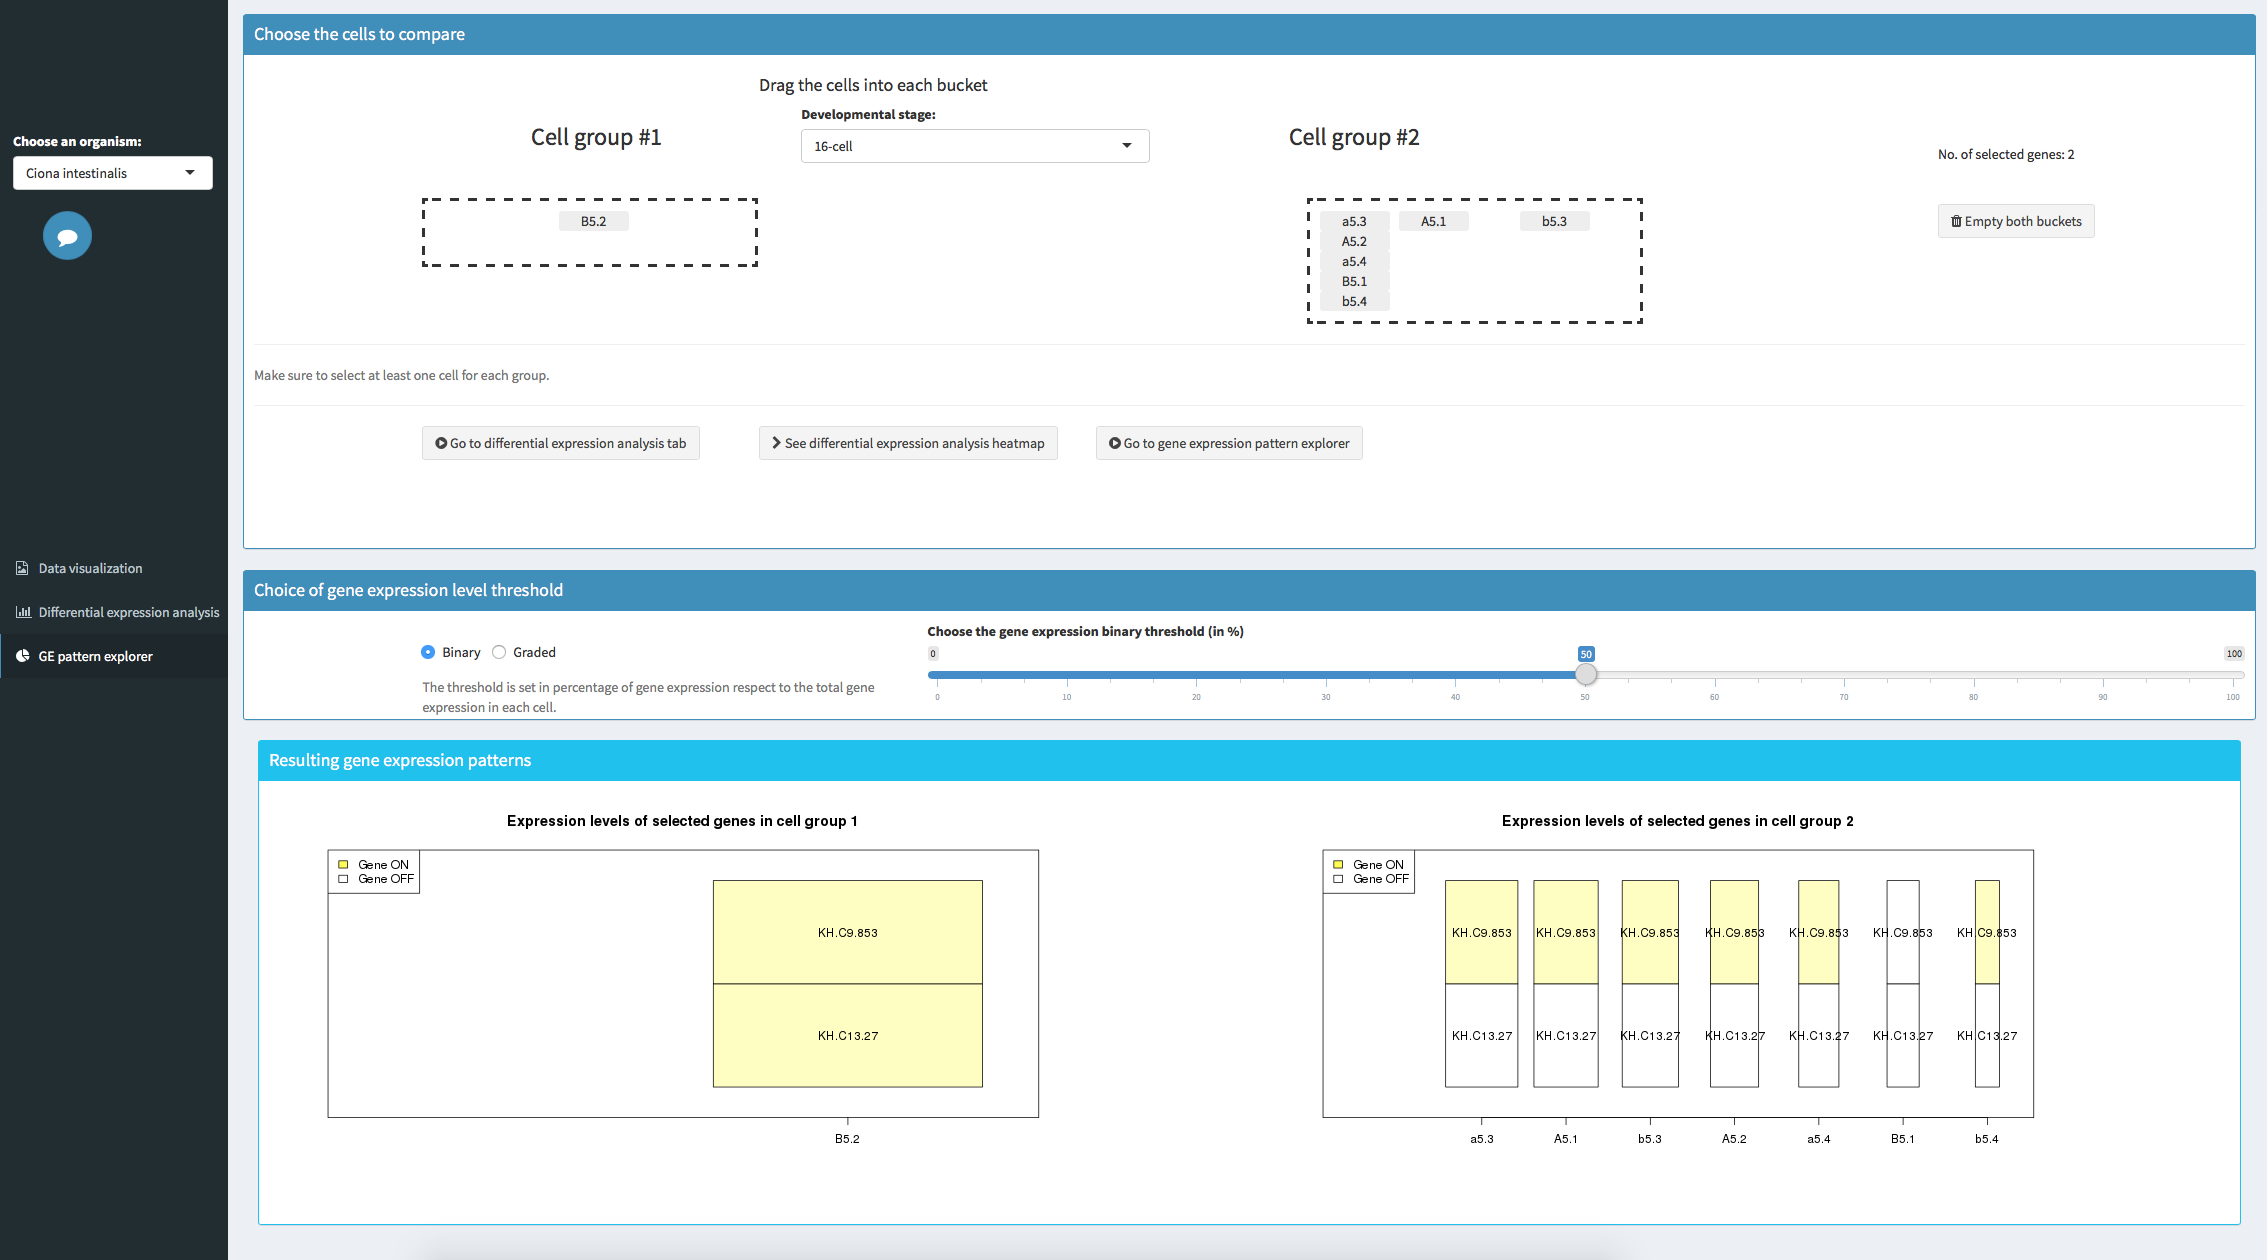
\includegraphics[scale=0.2]{application/patternthres2.png}
\caption{Visualization of gene expression pattern with selection of a binary gene expression threshold}
\label{visualization}
\end{figure}

\begin{figure}[H]
\centering
\subfigure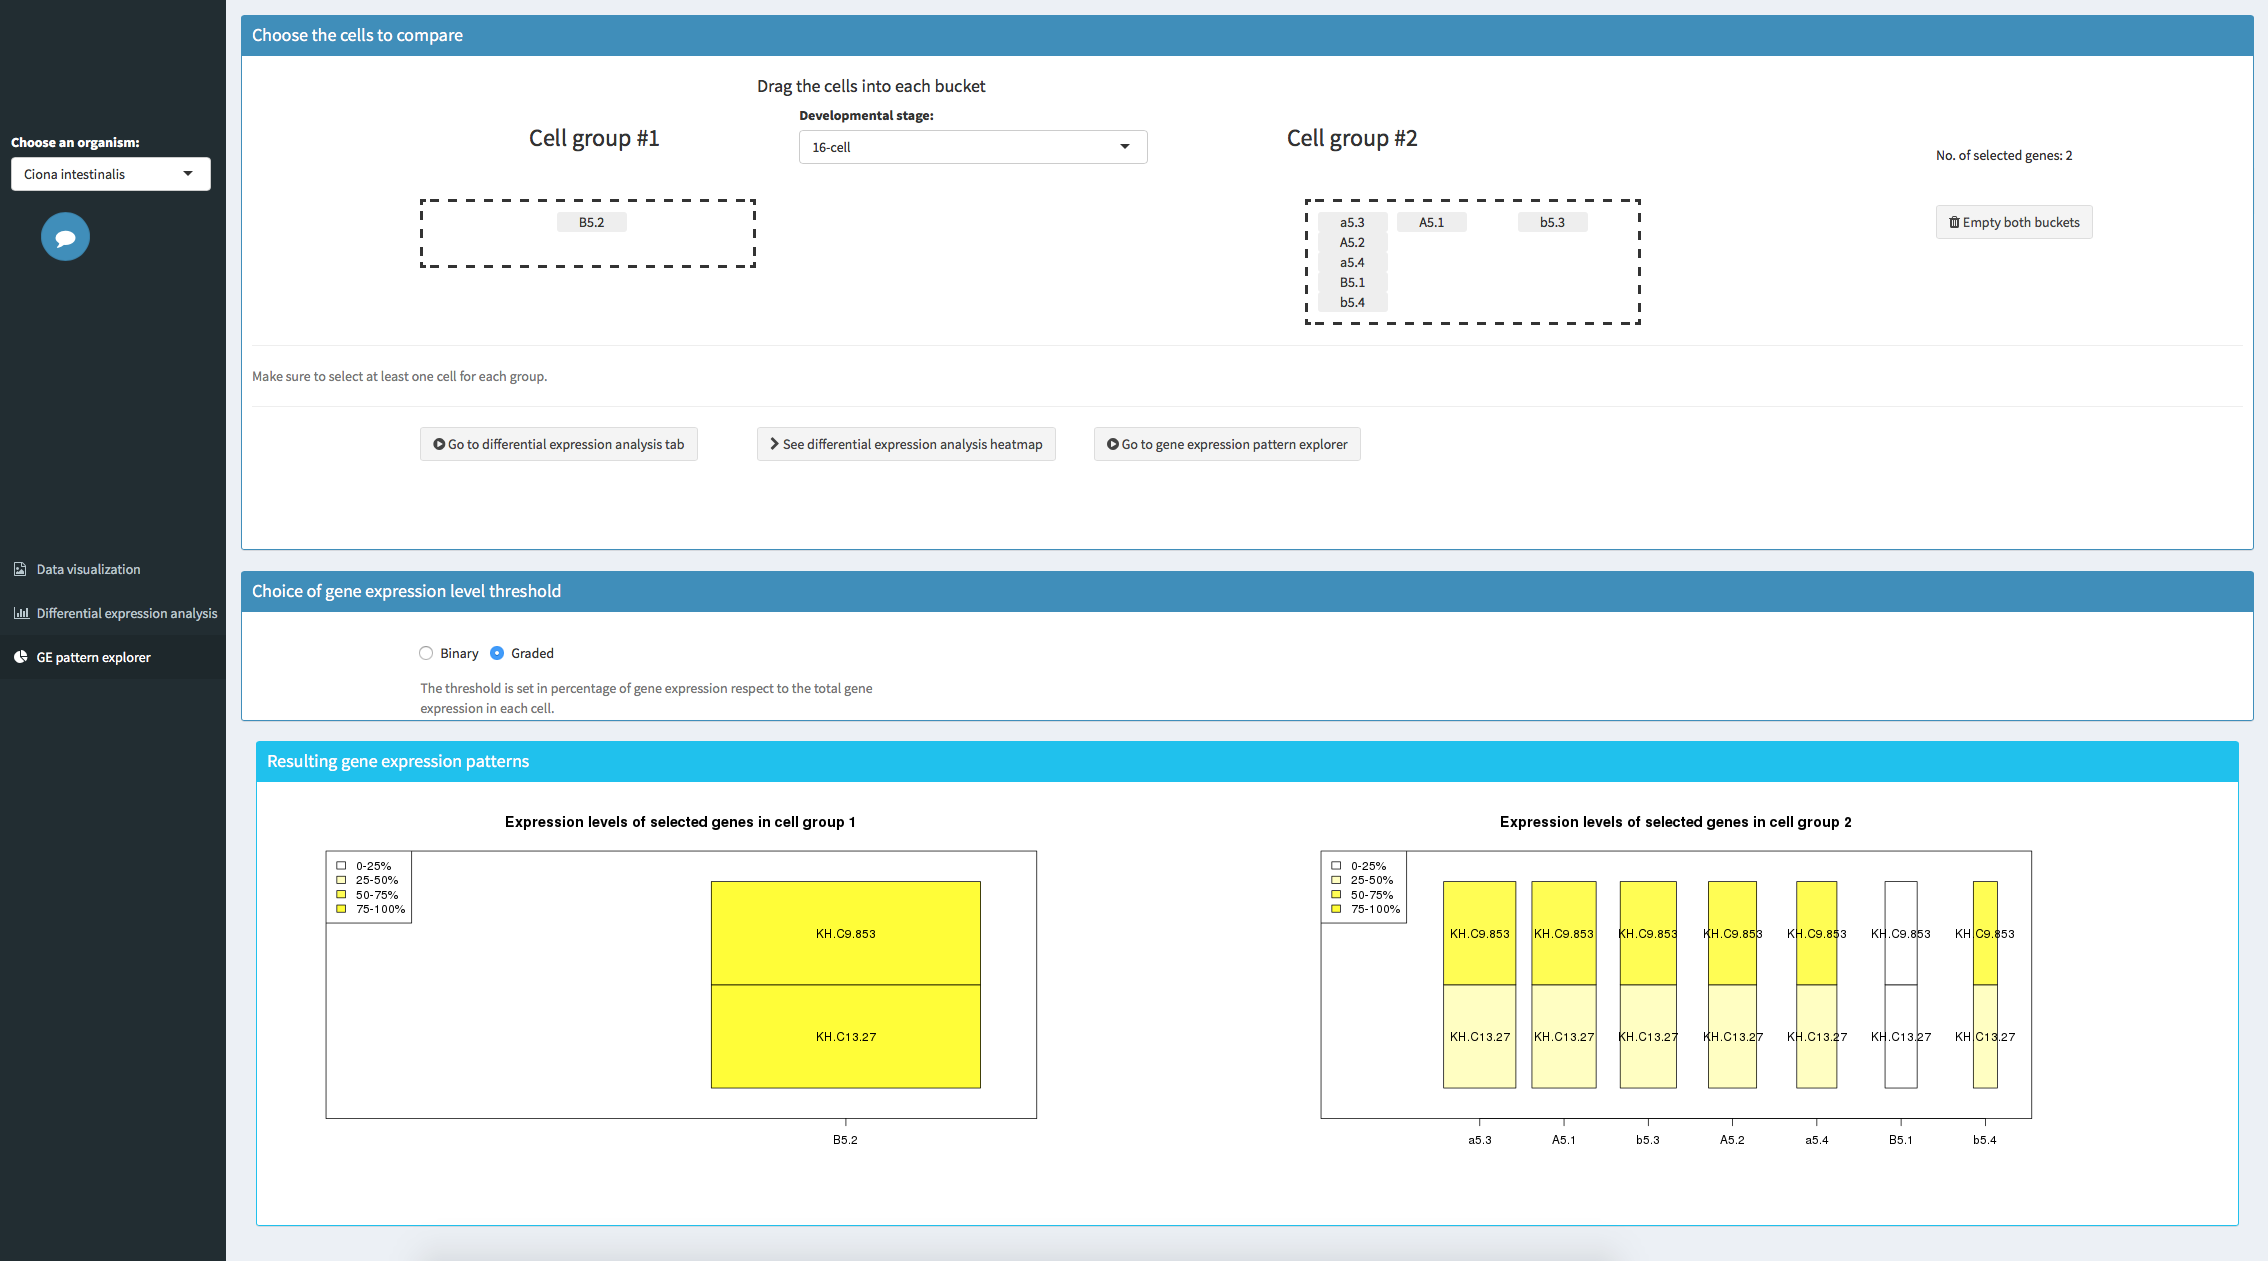
\includegraphics[scale=0.2]{application/gradedthres.png}
\subfigure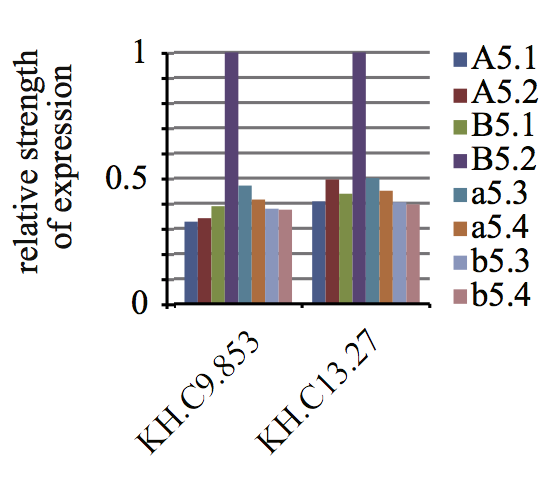
\includegraphics[scale=0.5]{application/figureDchordate.png}
\caption{Visualization of graded gene expression pattern and comparison with Figure B from \cite{matsuoka2013transcriptome}}
\label{graded}
\end{figure}

\chapter{Modeling of single-cell gene expression}

\textit{What determines the gene expression level for a given gene, in a given cell, for a given individual, who belongs to a given species?}\\

Because of the different factors (gene, cell, sequencing errors, etc.), trying to predict the absolutely exact gene expression count is indeed vain. However, being able to predict a relatively accurate gene expression value is enough for research purposes, and it has been studied intensively for data quality control softwares\cite{kharchenko2014bayesian}\cite{finak2015mast}\cite{love2014moderated}\cite{chen2014differential}. The model of gene expression is also implicitly chosen in the clustering algorithms.\\

However, such hypotheses as independence of gene expression between two genes, even in the same cell, are still widely assumed\cite{barash2002context}, even though they are clearly dismissed by the systems biology theory: genes \textit{do} interact with each other, favoring or inhibiting the expression of the other genes through regulatory paths. This assumption is also implicitly made by most of the algorithms introduced in Chapter 1 -except for Seurat\cite{satija2015spatial}.\\

To my knowledge, only \cite{barash2002context} (for microarray data), \cite{zhang2017classification} (for bulk RNAseq data) and \cite{satija2015spatial} (for scRNAseq data) have tried to tackle this issue.\\

However, \cite{barash2002context} models the gene dependency by \textbf{optimizing a cost function respect to} a certain set of intercorrelated feature classes denoted G (that is, finding a set G that minimizes a certain function), which is then used to generate posterior probabilities on the gene expression level of a certain gene (associated with random variable X) \textit{Prob}$(X | $class$ = k)$, which are computed differently depending on whether $k$ belongs to G, and the local structure associated with this class. This model seems hard to adapt to the specificities of scRNAseq data (see previous sections), and computationally expensive, since G, the local structures for each feature class in G, and the parameters of the posterior probability distributions need to be learned beforehand.\\

\cite{satija2015spatial}, although it is targeted at scRNAseq data, does not take into account the dropout phenomena, and needs to select a small subset of "landmark" (informative) genes (which are actually high-variance genes), and to compute "a spatial reference map of gene expression" for these genes. Moreover, the role of the "resolution" parameter is not intuitive, thus choosing a value for this parameter is done by trial and error. Sometimes, choosing the value in the interval [1,2], as suggested by the authors, does not give good results.\\

In \cite{zhang2017classification}, based on the work of \cite{hee2014copula}, the use of copulas, despite of not being directly adaptable to scRNAseq, is a more elegant solution, that allows to select separately the feature dependence model and each feature probability distribution. The flexibility of this sort of model offers the opportunity to better control and list the underlying  simplifying hypotheses.\\

What I want to find a model of gene expression associated to each condition of the gene expression matrix, that takes into account gene correlation. The set of expression values of all genes in a given cell can be aggregated into a real-valued vector. I will thus try to find a suitable copula model, associated with each condition, that is as close as possible to the multivariate cumulative distribution function giving the probability of the gene expression vector associated to this cell to be smaller (coordinate-wise) to some constant vector. The main point that justifies this approach is that little is known about the whole regulatory system between genes in one cell, but approximations of expression for one given gene have already been studied. Hence distribution models for each variable of the gene expression vector associated with one cell are known.

\section{Mathematical background}

Copulas are a efficient and simple tool to model correlation between random variables. 

\bigskip
\noindent \textbf{Notations}
\bigskip

Let $I=\{1, 2, ..., p\}, p \in \mathbb{N^*}$, and let $(X_i)_{i \in I}$ be the set of real-valued random variables which joint probability distribution $\mathbb{P}$ is to find. For each $i \in I$, let $f_{X_i}$ denote the \textbf{cumulative distribution function} (CDF) associated with the random variable $X_i$, i.e.:

\begin{definition}[Cumulative distribution function]\label{cdf}{The CDF $f_{X_i}$ associated with random variable $X_i$ is defined such as:\begin{center} $\forall x \in \mathbb{R}, \forall i \in I, f_{X_i}(x) =$ \textit{Prob}($X_i \leq x$)\end{center}}\end{definition}

Let eventually $f_{X_1, X_2, ..., X_p}$ be the CDF of the random vector $(X_1, X_2, ..., X_p)$. $f_{X_1, X_2, ..., X_p}$ is called the \textbf{joint CDF} of the variables $(X_i)_{i \in I}$, while each $f_{X_i}$, for $i \in I$, is the \textbf{marginal CDF} (or \textbf{margin}) associated with variable $X_i$.

\begin{warning}{As a general rule:\\$\forall x = (x_1, x_2, ..., x_p) \in \mathbb{R}^p, f_{X_1, X_2, ..., X_p}(x) \neq f_{X_1}(x_1) \times f_{X_2}(x_2) \times ... \times f_{X_p}(x_p)$}\end{warning}

Let |S| denote the cardinal of the set S. Let us recall that \textbf{mutual independence} in statistics, for a set of variables $(C_i)_{i \in I}$, means that the following equalities hold:

\begin{definition}[Mutual independence]\label{mutualindependence}{~ \\ \begin{center}$\forall J \subseteq I, \forall c = (c_j)_{|J|} \in \mathbb{R}^{\#J}, f_{(C_j)_{j \in J}}(c) = \prod{_{j \in J}}{f_{C_j}(c_j)}$\end{center}}\end{definition}

Mutual independence is distinct from regular (pairwise) independence, which means:

\begin{definition}[Pairwise independence]\label{independence}{~ \\\begin{center}$\forall i, j \in I, \forall c_1, c_2 \in \mathbb{R}, f_{C_i, C_j}(c) = f_{C_i}(c_1) \times f_{C_j}(c_2)$\end{center}}\end{definition}

If a random variable R follows the (continuous) standard uniform distribution $\mathbb{U}$, it means that:

\begin{definition}[Standard uniform distribution]\label{standarduniform}{~ \\\begin{center}$R \thicksim \mathbb{U}[0,1]$ iff. $\forall r \in $[0,1]$, f_{R}(r) = \mathbb{U}(R \leq r) = r$\end{center}}\end{definition}

\bigskip
\noindent \textbf{Copulas}
\bigskip

Generally speaking, a \textbf{copula}\cite{sklar1959fonctions} is a multivariate joint CDF whose margins are all continuous standard uniform distributions (an interesting explanation of copulas can be found in \cite{modellingcopulas}). The interest in copulas is motivated by Sklar's theorem\cite{sklar1959fonctions} (see \cite{carley2002new} for a proof):

\begin{theorem}[Sklar's copula theorem for real-valued random variables]\label{sklartheorem}{Let F be a multivariate cumulative distribution function (CDF), $p \in \mathbb{N}^*$ and $(X_i)_{i \in \{1, 2, ..., p\}}$ a set of random variables respectively following univariate distributions having CDF $(F_i)_{i \in \{1, 2, ..., p\}}$.\\

Then (if the $(F_i)_i$ are continuous) there exists (an unique) copula C such as: $\forall x_1, x_2, ..., x_p \in \mathbb{R}$, F($x_1, x_2, ..., x_p$) = C($F_1(x_1), F_2(x_2), ..., F_p(x_p)$).\\

Conversely, given a copula C, H : $(\mathbb{R}^+)^p$ $\rightarrow$ $[0,1]$, $x$ $\rightarrow$ $C(F_1(x_1), ..., F_p(x_p))$ is a CDF.}\end{theorem}

This theorem means that for any (unknown) multivariate CDF, one can generate values of this function using the marginal distributions of the random variables, provided a/the suitable copula has been selected, which is often easier than searching for the real multivariate function. The converse part means that any copula used with some univariate CDFs is a multivariate CDF, which allows to select a copula model and try to get a satisfying approximation of the target CDF.\\

I will use two lemmas:

\begin{lemma}[Mixture of copulas]\label{mixtureofcopulas}{A mixture of copulas is a copula, that is, if $C_1, C_2, ..., C_n$, where $n \in \mathbb{N}^*$, are copulas, and $\alpha_1, \alpha_2, ..., \alpha_n$ are positive real-valued numbers such as $\sum{_{i \leq n}}{\alpha_i} = 1$, then C : $[0,1]^n \rightarrow [0,1]$, $x \rightarrow \sum{_{i \leq n}}{\alpha_i \times C_i(x_i)}$ is a copula.}\end{lemma}

Since a copula is nothing but a multivariate CDF, the proof is easily deduced from elementary proofs in probability. The following lemma is also well-known:

\begin{lemma}[Probability integral transform]\label{cdfvariable}{Let R be a random variable with a continuous distribution, and $f_R$ be its continuous CDF. Then U = $f_R$(R) follows a standard uniform distribution.}\end{lemma}

Since copulas are essentially used to model dependence,  they are usually associated with a set of random variables. Let $p \in \mathbb{N^*}$ and $I = \{1, 2, ..., p\}$. Given a set of random variables $(X_i)_{i \in I}$, the corresponding copula is a multivariate function $C$ such as:

\begin{center}
C : $\mathbb{R}^p$ \rightarrow $[0,1]$, x \rightarrow C(f_{X_1}(x_1), f_{X_2}(x_2), ... , f_{X_p}(x_p)$)
\end{center}

This is well-defined thanks to \ref{cdfvariable}. \cite{unifmarginals} explains the importance of having standard uniform marginal distributions. The variables inside the copula are called \textbf{latent variables} associated with $(X_i)_{i \in I}$. Some plots about copulas and the relationship between the observed variables and the corresponding latent variables are be found in Appendix.\\

Hence the main purpose here is to make an assumption on the type of dependency between the variables, that is, the copula distribution (Gaussian, etc.) and then try to fit the chosen distribution to the data\cite{bedoui2008copules}. Copulas allows the separate modeling of the joint correlation and of the distributions of each vector component -however, modeling separately the distributions does not mean that their respective parameters should be chosen separately\cite{modelmarginaldependenceseparate}.\\

\bigskip
\noindent \textbf{Gaussian copulas}
\bigskip

Gaussian copulas are one of the simplest copulas. Let $C_{\rho}$ denote a Gaussian copula of parameter $\rho$, $\phi_{p(\rho)}$ being the multivariate normal distribution of zero-mean and standard deviation $\rho$, and $\phi$ being the standard normal distribution (of zero-mean and standard deviation 1). Then:

\begin{definition}[Gaussian copula]\label{gaussiancopula}{Let $(U_i)_{i \in I} = (f_{X_i}(X_i))_{i \in I}$ be a set of random variables following a standard uniform distribution, and C be the copula associated with the variables $(X_i)_{i \in I}$. Let $u \in [0,1]^p$. Then:\\$C_{\rho}(u_1, u_2, ..., u_p) = \phi_{p(\rho)}(\phi^{-1}(U_1) = \phi^{-1}(u_1), \phi^{-1}(U_2) = \phi^{-1}(u_2), ..., \phi^{-1}(U_p) = \phi^{-1}(u_p))$}\end{definition}

Thus I perform another variable transformation, as done in \cite{zhang2017classification}: I denote from now the latent variables $(Z_i)_{i \in I}$, such as $\forall i \in I, Z_i = \phi(f_{X_i}(X_i))$. 

\bigskip
\noindent \textbf{Estimation of the parameters}
\bigskip

I would like to compute the values of the parameters for the margin and copula functions -for instance, the mean vector and the covariance matrix for Gaussian copulas.  In order to find their values, the (log) \textbf{likelihood function} of the copula can be maximized, respect to the set of all parameters, but for Gaussian copulas, it has no closed form. There are many strategies to avoid this issue; for instance, a heuristic estimation method, called Inference Functions for Margins (IFM), suggested by \cite{joe1996estimation}, is to find the best estimators of the margin parameters, by maximizing the likelihood function of each of the margins, and then use them in the copula likelihood function to find the copula parameters with maximum likelihood estimation. This method is computationally less costly, and is considered a good heuristic method\cite{bouye2000copulas}, although it does not give the exact solution. Other methods also exist, see \cite{yan2007enjoy}.\\

Mainly in order to have a reasonable runtime, and avoid the problem of initialization for optimization methods, I decided to estimate the margin parameters and the copula parameters with provided non-optimization methods\cite{yu2013shrinkage}\cite{schafer2005shrinkage} (see Appendix for further information). These estimates are also proven to be more robust, and avoid the problem to deal with singularities when fitting the covariance matrix. This issue cannot actually be ignored, because gene expression matrices have usually a lot of null values, due to dropout events, for instance.\\

\section{Model}

Given a cell $j$, it models the probability distribution of expression level for a set of genes; let us number the set of considered genes. Let $X_j \in (\mathbb{R}^{+})^{p} = (X_{1,j}, X_{2,j}, ..., X_{p,j})$ be the random vector associated to the cell, where $X_{i,j}$ is the random variable associated to the expression level of gene $i$ in cell/condition $j$, and $p$ the cardinal of the set of genes. The probability distribution $\mathbb{P}_j$ of expression level in this cell is:

\begin{center}
\begin{equation}
\begin{split}
$\forall x \in (\mathbb{R}^{+})^{p}, \mathbb{P}_j(X_j = x) & =$ \textit{Prob}$(X_j = x)$\\ 
$& =$ \textit{Prob}$(X_{1,j} = x_1, X_{2,j} = x_2, ..., X_{p,j} = x_p)$
\end{split}
\end{equation}
\end{center}

\bigskip
\noindent \textbf{Main idea}
\bigskip

Considering their expression levels across all cells, genes can be divided in two groups: whether they have been subject to a dropout phenomenon. Considering their \textit{relative} expression values in a given cell, they can be divided into mildly-expressed and highly-expressed genes. I call \textit{cell pattern} the binary vector, having as many components as features in the dataset, where a case is set to 1 if the associated feature is considered highly-expressed in this cell, 0 otherwise.\\

The main assumption is, as written in one of the first sections, cell functions depends on the gene expression profile of the cell; thus I introduce the concept of cell pattern, which is close -in spirit- to the gene pattern implementation in \cite{satija2015spatial}. The gene expression probability distributions, for each cell, will depend on the cell patterns found, which is inspired by the probability distributions conditioned on gene classes like in \cite{barash2002context}.\\

\begin{figure}[H]
\centering
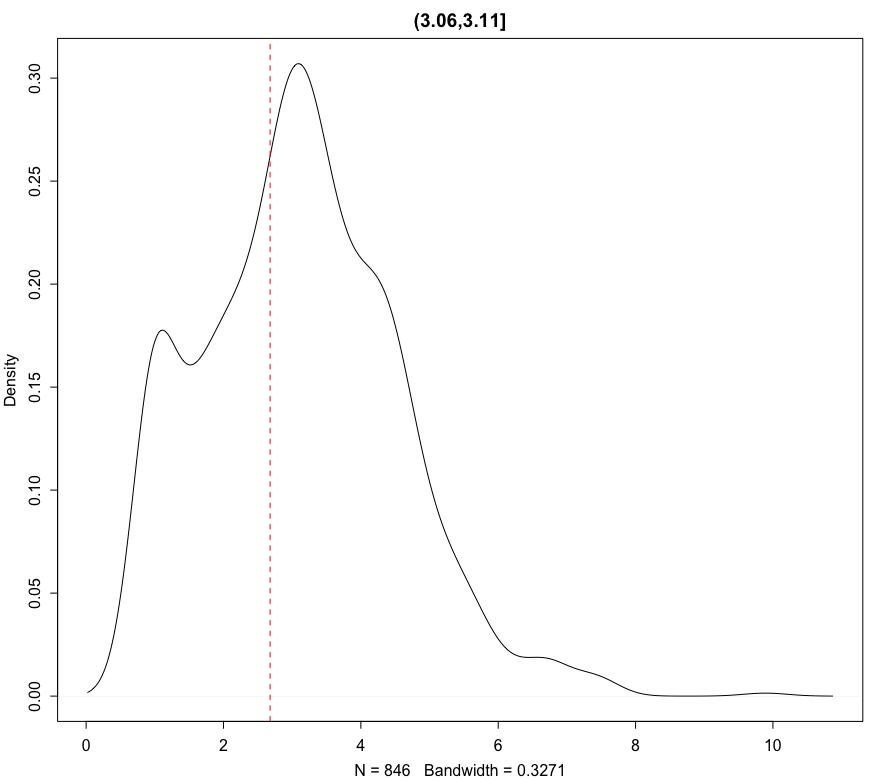
\includegraphics[scale=0.35]{illustrations/densityCionaLogNorm.png}
\caption{Result of kernel density estimation\cite{parzen1962estimation} (on n=846 points) applied on log-normalized gene expression values (that belong to the interval (3.06,3.11]) from the Ciona\cite{suyama2016singlecell} scRNAseq dataset. Kernel estimation is a method used to estimate the density function of a random variable (here, the expression value of a gene in a given cell) from a sample. The red vertical line is the threshold found by the MAST package (see next section).}
\label{densityCiona}
\end{figure}

The joint probability distribution of the expression levels for all genes in a given cell will be modeled with a copula specific to this cell, as done in \cite{zhang2017classification}. In order to tackle the problems specifically raised by scRNAseq data, I will use mixture probability distributions inspired by the works of \cite{kharchenko2014bayesian}, and \cite{finak2015mast} to model the marginal probability distributions for each gene in a given cell, depending on whether this gene is considered as dropout.\\

\bigskip
\noindent \textbf{Hypotheses}
\bigskip

\begin{enumerate}
\item \textbf{Mutual independence of gene expression values between different cells}:\\

\begin{center}
$\forall x, x' \in (\mathbb{R}^{+})^{p}, \forall k, l,\\ $\textit{Prob}$(X_k = x, X_l = x') = \mathbb{P}_k(X_k = x) \times \mathbb{P}_l(X_l = x') $
\end{center}

Note that this does not actually stand in practice (see plots in Appendix). But since the correlation between cell types is actually the point of gene expression clustering, there is no convincing prior hypothesis on cell correlation that does not imply using the cell labels.

\item \textbf{Non-independence of gene expression values between genes in a same cell}.\\

\item \textbf{Idea of a relationship between "cell pattern" and cell functions}: given a certain "activation threshold" and a certain cell, the set of genes that are expressed above this level (\textit{highly-expressed genes}, denoted by a 1 in the cell pattern) and genes that are expressed below this level (\textit{mildly-expressed genes}, denoted by a 0) is supposed to characterize the functional family of this cell.

\item All technical replicates (that is, cells from the same condition/embryo/stage/...) are supposed to follow the same gene expression value probability distribution.

\item Cells with a common functional role are supposed to have similar gene expression patterns (due to gene co-regulation\cite{barash2002context}).

\item \textbf{Hypotheses on the marginal and joint probability distribution models} (see following section "The distribution model").

\item \textbf{Mutual independence of the dropout events (resp. mild or high gene expressiveness events)}: this hypothesis is -implicitly- made about the dropout events in \cite{kharchenko2014bayesian}, when using binary logistic regression to determine the dropout probability for a given gene (see discussion for further insight on this hypothesis).
\end{enumerate}

\bigskip
\noindent \textbf{Notations}
\bigskip

\begin{itemize}
\item Let $|S|$ be the \textit{cardinal}, that is, the number of elements in the set S.
\item Let M be the input gene expression matrix of dimensions $p \times m$ (with $p >> m$), with features as rows, and conditions as columns. The set of rows for column $j$ is $(M_{i,j})_i$ = $\{M_{1,j}, M_{2,j}, M_{3,j}, ..., M_{p,j}\}$. The set of columns for row $i$ is $(M_{i,j})_j$ = $\{M_{i,1}, M_{i,2}, M_{i,3}, ..., M_{i,m}\}$.
\item As a general rule, the letter $i$ refers to a gene; the letters $j$ and $k$ refer to a condition or cell.
\item Let $(X_{i,j})_{i,j}$ = $\{X_{1,1}, X_{2,1}, ..., X_{p,1},$ $X_{1,2}, X_{2,2}, ..., X_{p,2}, ...,$ $X_{1,m}, X_{2,m}, ..., X_{p,m}\}$ be the set of nonnegative real-valued random variables associated to the counts $(M_{i,j})_{i,j}$ = $\{M_{1,1}, M_{2,1}, ..., M_{p,1},$ $M_{1,2}, M_{2,2}, ..., M_{p,2}, ...,$ $M_{1,m}, M_{2,m}, ..., M_{p,m}\}$. 
\item Let $\phi(\mu, \rho)$ be the multivariate cumulative function of a normal distribution with parameters (mean = $\mu$, variance = $\rho$), and $\phi$ the univariate standard normal distribution (of mean 0 and variance 1).
\item Let $P_k$ be the gene expression pattern for cell $k$, and $P$ be the matrix of all the gene expression patterns. 
\item For a certain cell $k$, let $Y_k$ be such as:

     \begin{center}
     $\forall i s.o. (P_k)_i = 1, (Y_k)_i = Y_ik = -(X_k)_i$\\
     $\forall i s.o. (P_k)_i = 0, (Y_k)_i = Y_ik = (X_k)_i$
     \end{center}

\item Let $f_{i,k} = f_{Y_{i,k}}$, and $f_k = f_{Y_{1,k}, ..., Y_{p,k}}$.
\item Let $Z_{i,k}$ the so-called latent random variable associated with $X_{i,k}$: $Z_{i,k} = \phi(f_{i,k}(Y_{i,k}))$, and $Z_k$ the latent random variable associated with $Y_k$: $Z_k$ = ($Z_{1,k}$, ..., $Z_{p,k}$).
\item Let $T_{i, j}$ denote the \textit{activation threshold} for cell $j$ and gene $i$, that is, one of the lowest points of the valley in Figure \ref{}, computed on normalized gene expression values, and let $Q$, called \textit{pattern-oriented threshold matrix} be defined such as $Q_{i,k} = T_{i, k}$ if $P_{i,k} = 0$, and $Q_{i,k} = -T_{i, k}$ otherwise.
\end{itemize}

\bigskip
\noindent \textbf{The distribution model}
\bigskip

The flexibility of the copulas allows the separate selection of the joint and the marginal distribution models. In my model, each cell is modeled by a copula, which is the joint probability distribution for the gene expression for all features in this cell. That is, the margins for each copula are associated to the expression value of each gene in the dataset. So here, each copula, associated with a given cell $j$, is the cumulative joint probability distribution function of gene expression value for each gene in cell $j$.

\bigskip
\noindent \textit{The marginal probability distribution (for each gene, in a given cell)}
\bigskip

Gene expression is subject to dropout phenomena\cite{kharchenko2014bayesian}, and is intrinsically bimodal\cite{finak2015mast}\cite{bessarabova2010bimodal} -and sometimes even multimodal\cite{ochab2010bimodal}.\\

According to \cite{kharchenko2014bayesian}, the most probable model for gene expression \textit{count} values (i.e. discrete values) $X_{i,j}$, for a given gene in a given cell, would be a mixture of a low-magnitude Poisson distribution, to model the gene expression values subject to dropout, and negative-binomial distribution, to take into account the overdispersion of gene expression values for a successful amplification, using as mixing rate the dropout probability for this gene in this cell:

\begin{definition}[Discrete gene expression value model]\label{genexpressiondiscrete}{Let $p_{i,j}$ be the dropout probability for gene $i$ in cell $j$. Then:
\begin{center}$\forall x \in \mathbb{N}, $\textit{Prob}$(X_{i,j} = x) = p_{i,j} \times $\textit{Poisson}$(\lambda_{i,j}) + (1-p_{i,j}) \times $\textit{NegBin}$(r_{i,j}, p_{i,j})$\end{center}}\end{definition}

where the density functions for Poisson and negative-binomial distributions are respectively:

\begin{definition}[Poisson distribution]\label{poisson}{~\\\begin{center}$\forall X \thicksim$ \textit{Poisson}$(\lambda), \forall k \in \mathbb{N},$ \textit{Prob}$(X = k) = \frac{\lambda^k \times e^{-\lambda}}{k!}$\end{center}}\end{definition}

\begin{definition}[Negative binomial distribution]\label{negativebinomial}{~\\\begin{center}$\forall X \thicksim$ \textit{NegBin}$(r, p), \forall k \in \mathbb{N},$ \textit{Prob}$(X = k) = {{k+r-1}\choose{k}} \times (1-p)^r \times p^k$\end{center}}\end{definition}

When a gene is subject to a dropout phenomenon, only low background noise is detected. As done in \cite{kharchenko2014bayesian}, instead of using constant zero function, I take into account random background noise by setting the Poisson parameter to a low constant:

\begin{center}
$\forall i,j \in \{1, 2, ... p\} \times \{1, 2, ..., m\}, \lambda_{i,j} = \lambda_0 < 1$\\
\end{center}

Instead of using $r$ and $p$ parametrization for the Negative Binomial distribution, I use the mean-overdispersion ($\mu, \delta$) parametrization for negative-binomial\cite{rodriguez2013models}, which is easier to interpret (see Appendix for the equivalence between the two parametrizations).\\

However, the marginal distributions need to be continuous in order to use a copula -and to estimate its parameters more easily. It is not continuous now since the Poisson and Negative binomial distributions are discrete. Furthermore, I need to model also the gene expression values when the values are normalized, so not necessarily integers anymore. And the Poisson distribution (thus the Negative Binomial one, since the latter is a mixture of Poisson and Gamma distributions) is sensible to scale modifications.\\

Thus I use a standard Gamma distribution, that is, with shape parameter $\lambda$, and rate parameter 1, to model the Poisson distribution, and a regular Gamma distribution, with parameters $\alpha$ (shape) and $\beta$ (rate) for the Negative Binomial distribution (Gamma distribution has been actually widely studied as an approximation for this distribution\cite{guenther1972simple}\cite{best1974improved}), where the density function for a Gamma distribution is:

\begin{definition}[Gamma distribution]\label{gamma}{~\\\begin{center}$\forall X \thicksim \Gamma(\alpha, \beta), \forall x \in \mathbb{R}^+,$ \textit{Prob}$(X = x) = \frac{\beta^{\alpha} \times x^{\alpha-1} \times e^{-\beta \times x}}{\Gamma(\alpha)}$\end{center}}\end{definition}

Again, the selection of the mean and the (over)dispersion factor ($\mu, \delta$) boils down to select parameters ($\alpha, \beta$) (see Appendix). Henceforth the marginal distribution for gene expression and variable $X_{i,j}$ is:

\begin{definition}[Continuous gene expression value model)]\label{genexpressioncontinuous}{Let $p_{i,j}$ be the dropout probability for gene $i$ in cell $j$. Then:
\begin{center}$\forall x \in \mathbb{N}, $\textit{Prob}$(X_{i,j} = x) = p_{i,j} \times $\textit{Gamma}$(\lambda_0, 1) + (1-p_{i,j}) \times $\textit{Gamma}$(\mu_{i,j}, \delta_{i,j})$\end{center}}\end{definition}

I will call this probability distribution CPNB($\lambda_0, p_{i,j}, \mu_{i,j}, \delta_{i,j}$) (continuous -approximation of- Poisson-Negative Binomial mixture).

\bigskip
\noindent \textit{The copula probability distribution (for each cell)}
\bigskip

According to the general assumption about the relationship between cell functions and gene expression profile, and the plots in Appendix, I can choose as starting distribution a bimodal Gaussian copula, that is, a mixture of two Gaussian copulas (such a mixture is a copula, see Lemma \ref{mixtureofcopulas}). The one with the highest mean is most likely associated with the most highly-expressed genes in the cell, while the second one seems to match the less expressed genes, which agree with my idea of cell gene expression pattern. I use the same assumption as \cite{zhang2017classification} (which will be discussed later), that is, the covariance matrices represent the regulatory interactions between the genes, thus I assume that both copulas in a mixture have got the same covariance matrix, and that this matrix is independent of the considered cell.\\

I denote such a bimodal Gaussian copula of means $\mu_1, \mu_2$, with mixing parameter $\alpha$ and covariance matrix $\Sigma$, $C_{\mu_1, \mu_2, \alpha, \Sigma}$.\\

Please keep in mind that the variables associated with the copulas are $(Y_{i,j})_{i \leq p, j \leq m}$ (see notations), because what I want to compute is the probability of each gene to have an expression value above or below their associated activation threshold (see the following sections). Since for all $i,j \in \{1,2,...,p\} \times \{1,2,...,m\}$, $Y_{i,j} = X_{i,j}$ if $P_{i,j} = 0$, and $Y_{i,j} = -X_{i,j}$ otherwise, the associated marginal cumulative distributions $f_{Y_{i,j}}$ are easy to deduce from the previous section (see Appendix). The latent variables associated are thus, for all $k \leq m$, $(Z_{i,k})_{i \in I} = (\phi(f_{Y_{i,k}}(Y_{i,k})))_{i \in I}$.

\bigskip
\noindent \textit{The final model}
\bigskip

For each cell, the final copula distribution model is:

\begin{definition}[Final gene expression distribution model]\label{cellcopula}{Let $j$ be the index of a given cell in the dataset. If $q$ is a vector of gene expression in this cell ($q \in \mathbb{R}^{+p}$):\begin{center} 
\textit{Prob}($Y_j \leq q$) = $C_j_{\mu_1_j, \mu_2_j, \alpha_j, \Sigma}(Z_{1,j} \leq \phi(f_{Y_{1,j}}(q_1)), Z_{2,j} \leq \phi(f_{Y_{2,j}}(q_2)), ..., Z_{p,j} \leq \phi(f_{Y_{p,j}}(q_p)))$\end{center}}\end{definition}

To know more about the parameter value estimation, see Appendix.

\bigskip
\noindent \textbf{Cell comparison}
\bigskip

Now that I have defined a gene expression value probabilistic model, that focuses on the \emph{relative} gene expression levels, to tackle the issue highlighted in the introduction, I would like to be able to compare gene expression profiles between cells, to perform cluster analysis. Intuitively, I consider two cells to be similar if they have the same cell pattern, as computed in matrix P, and the more the probability -implicitly conditioned on the parameters of the distribution model- of both gene expression profiles having this pattern is high, the more they are similar (see last part of this section for a discussion of this hypothesis). This intuition arises from the fact that cells are usually considered similar if they exhibit gene expression "trend similarity"\cite{jaskowiak2014selection}, that is, similar gene expression profiles (i.e. the proportions of gene expression are roughly the same). That would mean that they have similar functions.\\

\begin{definition}[Gene expression profile and cell pattern]\label{profilepattern}{A gene expression profile G -a $p$-sized nonnegative real-valued vector- suits a given pattern P -$p$-sized binary vector- respect to threshold vector T -a $p$-sized nonnegative real-valued vector- if and only if:\begin{center}
$\forall i \in \{1,2,...,p\},$ if $P_i = 1$, then $G_i > T_i$, and otherwise $G_i \leq T_i$\end{center}}\end{definition}

\begin{definition}[Cell similarity]\label{cellsimilarity}{Let $k,l$ be two cells. $k$ and $l$ are similar iff:\\
\begin{enumerate}
\item $k = l$
\item The probability of the event "$\forall i \in \{1,2,...,p\}, P_{i,k} = P_{i.l}$ and\\- either $P_{i,k} = 1$ and $X_{i,k} > T_{i}, X_{i,l} > T_{i}$,\\- or either $P_{i,k} = 0$ and $X_{i,k} \leq T_{i}, X_{i,l} \leq T_{i}$" is "high enough".
\end{enumerate}}\end{definition}

Let us try to figure out how to compute similarity value in the second case. Let $I = \{1,2, ...,p\}$, $U_0 = "\forall i \in \{i \in I | P_{i,k} = 0\}, X_{i,k} \leq T_i, X_{i,l} \leq T_i"$, and $U_1 = "\forall i \in \{i \in I | P_{i,k} = 1\}, X_{i,k} > T_i, X_{i,l} > T_i"$. These events can be rewritten with random variables $(Y_{i,k})_{i,k}$ and real numbers $(Q_{i,k})_{i,k}$ (see previous section about the notations). I use the pairwise coordinate order on vectors:

\begin{center}
\begin{equation}
\begin{split}
\textit{Prob}($U_1$ AND $U_0$)
$& =$ \textit{Prob}($\forall i \in I, Y_{i,k} \leq Q_{i,k}$ AND $Y_{i,l} \leq Q_{i,l})$\\
$& =$ \textit{Prob}($Y_{k} \leq Q_{k}$ AND $Y_{l} \leq Q_{l})$\\
$& =$ \textit{Prob}($Y_{k} \leq Q_{k}$) \times \textit{Prob}($Y_{l} \leq Q_{l})$\\
\end{split}
\end{equation}
using assumed cell mutual independence.
\end{center}

\begin{definition}[Cell similarity measure]{Let $k,l$ be two cells. Then their similarity value $sim(k,l)$ (0 being complete dissimilarity, and 1 being identity) is defined as such:\\
- if $k=l$, then $sim(k,l) = 1$\\
- else if $P_k \neq P_l$ (i.e. $\exists i \in \{1,2, ..., p\}, P_{i,k} \neq P_{i,l}$), then $sim(k,l) = 0$\\
- else $sim(k,l) =$ \textit{Prob}$(Y_k \leq Q_k) \times$ \textit{Prob}$(Y_l \leq Q_l)$}\end{definition}

\newpage

\section{Clustering method}

The algorithm I suggest is a model-based hierarchical clustering algorithm\cite{fraley2002model}, that is, it tries to infer the similarities between elements by modeling the distribution generating each group. Copulas have actually already been used for clustering/classification\cite{stitou2009copulas}\cite{kosmidis2014model}, and recently were applied to RNA-seq data classification\cite{zhang2017classification}.\\

Mine is divided in five parts, which details can be found in Appendix. I will use the same notations defined in the last section.

\bigskip
\noindent \textbf{Input}
\bigskip

This algorithm takes as input:\\

\begin{itemize}
\item The (un)normalized gene expression matrix.
\item A cell-wise similarity threshold $d$: it is meant to be the threshold for the probability of two cells to be similar, in the sense I described above. The default value is 0.5.
\end{itemize}

There are also other values used for clustering and feature selection, that can be modified:

\begin{itemize}
\item $d_{neighbors}$, which is a threshold for merging cell pattern clusters (default: $d$): the cell-neighbor similarity threshold required for agreement of the neighbor (see Appendix). This value can modified to allow double thresholding, according to the importance of having homogenous clusters.
\item $d'$, which is the threshold for gene correlation: two genes are considered truly correlated if their correlation number is above $d'$, and their mean gene expression value is roughly similar (see Appendix). Default value is 0.9, but 0.75 is the minimum generally allowed\cite{featureselectioncaret}.
%\item $d_{pattern}$: two patterns are considered equal if they have at least $d_{pattern} \times 100$ \% of common components.
\item $f$, such as if a gene appears in more than $f \times 100$ \% of the conditions, then it is considered ubiquitous and removed. Default value is 0.7, which is a rough guess based on experimental data.
\end{itemize}

\bigskip
\noindent \textbf{Outlines}
\bigskip

\begin{algorithm}[H]
\caption{Clustering technique: \textbf{Mine} algorithm}
\begin{algorithmic}
\STATE \textbf{Input}: M, gene expression matrix of size $p \times m$
\STATE \textbf{Parameters}: 
\STATE - $d$, probability threshold for merging cell patterns (default: 0.5)
\STATE \textbf{Hidden parameters}: 
\STATE - $d_{neighbors}$, threshold for merging cell pattern clusters (default: $d$)
\STATE - $d'$, threshold for gene correlation (default: $0.9$)
%\STATE - $d_{pattern}$ (default: 0.9)
\STATE - $f$ (default: $0.7$)
\STATE \textbf{Output}: clustering of the conditions (columns) in matrix M
\STATE \textbf{---------------------Pre-processing---------------------}
\STATE $M \leftarrow$ filter(M)
\STATE $M \leftarrow$ featureSelect(M)
\STATE $M \leftarrow$ frequenceTrim(M)
\STATE \textbf{---------------------Finding pattern---------------------}
\STATE $res \leftarrow$ thresholdComputation(M)
\STATE $modelDropout, modelMild, P, Q \leftarrow$ getPatterns(M, res)
\STATE \textbf{---------------------Distribution computation---------------------}
\STATE $margin\_means, margin\_deltas, margin\_rates \leftarrow $estimateMarginParameters$(M, P, modelDropout)$
\STATE $copulas \leftarrow$ \textbf{NULL}
\FOR{$j \in \{1, 2, 3, ..., m\}$}
\STATE $copulas\_j \leftarrow $createBimodalCopula$(M, modelMild)$
\ENDFOR
\STATE \textbf{---------------------Merging pattern---------------------}
\STATE $distMatrix \leftarrow$ null matrix of order $m$
\STATE \textbf{\# The elements in the max heap are sorted by similarity value \#}
\STATE $mergeablePairs \leftarrow$ initializeHeap()
\FOR{$k \in \{1, 2, 3, ..., m-1\}$}
\FOR{$l \in \{k+1, k+2, k+3, ..., m\}$}
\STATE $sim \leftarrow $computeSimilarity$(k, l, copulas\_k, copulas\_l, P, Q)$
\STATE $distMatrix[k][l] \leftarrow$ 1-$sim$
\STATE $distMatrix[l][k] \leftarrow$ 1-$sim$
\IF{$sim > d$}
\STATE pushHeap($k,l$)
\ENDIF
\ENDFOR
\ENDFOR
\STATE \textbf{---------------------Clustering---------------------}
\STATE $clusters \leftarrow$ initializeClusters()
\WHILE{no cluster convergence}
\STATE $queue \leftarrow$ mergeablePairs\\
\WHILE{ \textit{queue} is not empty}
\STATE $k,l \leftarrow$ extractMinHeap(\textit{queue})
\IF{$k$ and $l$ are in distinct clusters}
\IF{there is agreement between the neighbors of $k$ and $l$}
\STATE merge the clusters of $l$ and $k$
\ENDIF
\ENDIF
\ENDWHILE
\ENDWHILE
\RETURN{\emph{clusters}}
\end{algorithmic}
\end{algorithm}

\bigskip
\noindent \textbf{Discussion of the model}
\bigskip

\begin{itemize}

\item Instead of the regular mixture model I have chosen, I could have used a zero-inflated model (ZIM)\cite{rodriguez2013models}. A ZIM is, given a density distribution function $f$, a mixture rate $0 < \alpha < 1$, and a nonnegative real-valued random variable R, the associated ZIM is defined such as:

\begin{definition}[General zero-inflated model]\label{zeroinflated}{ ~\\
\begin{center} \textit{Prob}($R = 0$) = $\alpha + (1-\alpha) \times f(0)$ \end{center}
\begin{center} $\forall r \in \mathbb{R}^+, r > 0$ \textit{Prob}($R = r$) = $(1-\alpha) \times f(r)$ \end{center}
}\end{definition}

Note that it is in fact a mixture model with a given probability distribution (Negative Binomial alike for instance) and the null distribution. But, as written previously, contrary to the null distribution, the Poisson distribution allows to account for low background noise\cite{kharchenko2014bayesian}, if its parameter value is low enough.\\

Another issue of my model is that I have to compute the best value for the mixture rate parameter. The hurdle (most of the time set at zero) model is a way to overcome this problem; given two density distribution functions $f_1$ and $f_2$ to mix, and a nonnegative real-valued random variable R, the associated hurdle model is\cite{arnold2009advances}:

\begin{definition}[General hurdle model]\label{hurdlemodel}{ ~\\

\begin{center} \textit{Prob}($R = 0$) = $f_1(0)$ \end{center}
\begin{center} $\forall r \in \mathbb{R}^+, r > 0$ \textit{Prob}($R = r$) = $\frac{1-f_1(0)}{1-f_2(0)} \times f_2(r)$ \end{center}
}\end{definition}

For instance, $f_1$ would be the Poisson density function, and $f_2$ be the Negative Binomial density function. But note that this model assumes that the dropout part (that is, the Poisson component of the mixture) is the only one source of null gene expression values. But I consider that transcriptionally silent genes, that is, whose sequence does not appear in the mRNA molecule, also give quasi-zero values\cite{kharchenko2014bayesian}. 

\item I could have used the two continuous counterparts of Poisson and Negative Binomial built by \cite{ilienko2013continuous}\cite{chandra2012continuous}\cite{abid2016continuous}, but they are computationally expensive, and since I just want to fit the data, I do not need the asymptotic limits of the probability distributions, but only the assumptions made on variance and mean (and not median, for instance). Estimation of the parameters for copulas is easier when the marginals are continuous, especially for the computation of the gradient needed for optimization procedures.\\

Gamma distribution is also quite close to Poisson and Negative Binomial distributions, and has already been used as an approximation for both of them, see \cite{best1974improved}\cite{guenther1972simple}. I cannot assume that the gene expression values of the two gene groups (dropout and non-dropout) are independent, thus the mixture of the two Gamma distributions is not necessarily a Gamma distribution.

\item The Gaussian copula for one-cell gene dependence is probably a really rough assumption. But it is the most recommended for general models\cite{inouye2017review}, and the real gene correlation model is not known. Moreover, since the number of dimensions is huge, the Gaussian copula is the easiest model to fit to the data, and there are efficient and accurate estimators of its parameters. 

\item The cell comparison measure suggested is not a distance -the given definition does not satisfy transitivity condition- and it may look a bit clumsy since it does not comply with the reflexivity property \emph{per se}. The main purpose of this definition is to be intuitively close to what I would expect in a cell clustering.\\

The problem lay upon the computation of the probability of having such a gene pattern for each of the cells. The model actually assumes that the true distribution of the gene expression is a mixture of Gamma distributions, and if the empirical distribution from the data does not abide by this assumption, the gene pattern will be considered unlikely to appear, thus a cell can be considered not similar to itself, and no clustering will actually make sense. This discrepancy may either come from bad quality data -but, with new technologies developing, it will be hopefully unlikely to happen- or either from the fact that the commonly used model for real gene expression is in fact not suitable.\\

\item Another issue is that the parameters are fitted on the very same data on which the clustering part will be applied. Ideally, the data would have lots of replicates of each condition/cell, and cross validation procedures could be performed. It though requires data annotation work. I tried to solve this issue by generating data using kernel density estimation, or by applying a Gaussian random noise to the input data.\\

A possible improvement would be the possibility to select a given number of cell groups, and to perform the clustering on these groups, e.g., cells from healthy people, from cancer-afflicted non-treated patients, and from treated patients. But the algorithm is meant to contribute to an exploratory analysis, thus seeing similarities between cells without prior hypothesis nor knowledge.

\item I assumed the covariance matrix was the same for every cell/copula, as done in \cite{zhang2017classification}. This covariance matrix is meant to represent the gene regulatory system network, as highlighted by \cite{schafer2005shrinkage}. This system is not supposed to be different from one cell to another. However, it might be different between a group of highly-expressed genes and a group of mildly-expressed genes.

\end{itemize}

\section{Implementation}

The algorithm has been implemented in R, and the source code can be found here: {\url{https://github.com/oist-gene-clustering/mine}}\\

Packages: R\cite{baser}, MAST\cite{mastr}, doParallel\cite{doparallelr}, mvtnorm\cite{mvtnormr}, caret\cite{caretr}, Matrix\cite{matrixr}, corpcor\cite{corpcorr}, fastcluster\cite{fastclusterr} and foreach\cite{foreachr}.\\

\chapter{Benchmark on clustering algorithms}

There exist currently lots of algorithms, each of them using various methods, developed to tackle cell clustering for single-cell RNA data, even through it is still quite a recent field. However, none of them has been selected yet as the reference clustering algorithm. I performed a benchmark, including the most known algorithms in R targeted at scRNAseq data, in order to compare the clustering results, and to check the correctness of the resulting functional cell families found.\\

The tested algorithms in the following benchmark are SC3, pcaReduce, tSNE+K-means, tSNE+DBSCAN, K-means, SNN-Cliq, SINCERA, SEURAT, NMF and Fuzzy C-means, and have been briefly introduced in the section \textbf{Cluster analysis}.\\

\section{Pipeline}

\bigskip
\noindent \textbf{Method}
\bigskip

This benchmark tests the ability of one algorithm to find consistent clusters of cells/conditions (\textbf{accuracy test}), respect to the biological data, the time needed to compute the answer in function of the dimensions of the gene expression matrix (\textbf{time complexity test}), and the stability of the resulting clustering (\textbf{stability test}). For more insight on the datasets, see Appendix.\\

For each dataset, I looked up in the corresponding article the expected number of clusters, and tried to find a "reference clustering", that is, the annotation of the subpopulations in the dataset. Sometimes the number of clusters does not match the number of subpopulations, but I assumed that the annotation into subpopulations is still either a subclustering or a overclustering of the real reference clustering, and thus could be helpful to determine if the algorithm gave consistent results with the data. For more details about the data, please check the Excel file at the following link: {\url{https://github.com/oist-gene-clustering/geneclusteringbenchmark}}\\ 

To be able to compare fairly the different algorithms, I tried to find the best parameters for each dataset and each algorithm (which can be found in the Excel file previously quoted), that is, which seemed to give the best results according to the PCA and tSNE plots, and giving a number of clusters as close as possible to the expected one. Of course, these plots can only be considered indications and have bias, but since I could not get access to the real reference clustering, I thought it would be wiser not to rely too much on the latter.\\

Eventually, I ran again several times all the algorithms on one dataset (the one having the highest mean accuracy measure), in order to observe the variation of accuracy between runs.

\bigskip
\noindent \textit{Accuracy test}
\bigskip

I tested on each dataset each algorithm. For indeterministic algorithms, I used 100 runs and kept the clustering giving the highest Adjusted Rand Index\cite{rand1971objective} (ARI, computed with MClust\cite{fraley1999mclust}) with the reference clustering I fixed for each dataset. Except for Seurat, SINCERA and SNN-Cliq, all algorithms are indeterministic. 

\begin{definition}[Adjusted Rand Index (ARI)]\label{ARI}{
Let $X = \{X_1, X_2, ..., X_r\}$ and $Y = \{Y_1, Y_2, ..., Y_s\}$ be two clusterings of the same dataset $\{x_1, x_2, ..., x_m\}, m, r, s \in \mathbb{N^{*}}$. For all $k,l \in \{1,2,...,r\} \times \{1,2,...,s\}$, let $n_{k,l} = |X_k \cap Y_l|$ be the number of common points in clusters $X_k$ and $Y_l$, and $a_k = \sum{_{l \leq s}}{n_{k,l}}$, and $b_l = \sum{_{k \leq r}}{n_{k,l}}$. Then:}\end{definition}\\

\begin{center}
$ARI(X, Y) = \frac{\sum{_{i,j}}{{n_{i,j}}\choose{2}} - (\sum{_i}{{a_i}\choose{2}} \times \sum{_j}{{b_j}\choose{2}})/{{m}\choose{2}}}{\frac{1}{2} (\sum{_i}{{a_i}\choose{2}} + \sum{_j}{{b_j}\choose{2}}) - (\sum{_i}{{a_i}\choose{2}} \times \sum{_j}{{b_j}\choose{2}})/{{m}\choose{2}}}$
\end{center}

The ARI may take negative values, meaning that the resulting accuracy respect to the reference clustering is less than the expected index when the compared clustering has been generated randomly. The closer it gets to 1, the more the two clusterings are similar. This measure is commonly used for clustering comparison, as done in \cite{kiselev2016sc3}\cite{jaskowiak2014selection}, for instance.\\

\bigskip
\noindent \textit{Time complexity}
\bigskip

The benchmark takes into account the time (in seconds, using base R function \emph{system.time}) needed to compute the solution with the highest ARI.

\bigskip
\noindent \textit{Stability test}
\bigskip

Indeterministic algorithms have been iterated 100 times on the Biase dataset. Then I computed a stability measure, which is the frequency among the 100 runs of the most frequent solution. It may show the difference of performance between two iterations of the same algorithm on a given dataset.

\section{Results}

See Appendix for more details about the ranking.

\begin{table}[H]
\centering
\caption{Ranking of algorithms (the "average" value is computed using the weighted mean described in Appendix)}
\begin{tabular}{| l | l | l | l | l |}
\hline
\parbox[c]{2cm}{\textbf{Rank}} & 
\parbox[c]{3cm}{\textbf{Accuracy\\(ARI)}} & 
\parbox[c]{3cm}{\textbf{Accuracy\\(absolute(no.\\clusters-expected no.))\\}} & 
\parbox[c]{3cm}{\textbf{Stability}} &
\parbox[c]{3cm}{\textbf{Time}}\\
\hline
\parbox[c]{2cm}{\textbf{\#1}} & 
\parbox[c]{3cm}{Fuzzy C-Means\\(avg. ARI: 0.77)} & 
\parbox[c]{3cm}{SC3\\avg. abs. diff: 0)} & 
\parbox[c]{3cm}{SC3\\(stability: 1.00)} &
\parbox[c]{3cm}{+DBSCAN\\(avg. time: 4.97s)}\\
\hline
\parbox[c]{2cm}{\textbf{\#2}} & 
\parbox[c]{3cm}{K-Means\\(avg. ARI: 0.74)} & 
\parbox[c]{3cm}{+K-means\\(avg. abs. diff: 0)} & 
\parbox[c]{3cm}{PCAReduce\\(stability: 0.29)} &
\parbox[c]{3cm}{SINCERA\\(avg. time: 6.00s)}\\
\hline
\parbox[c]{2cm}{\textbf{\#3}} & 
\parbox[c]{3cm}{SC3\\(avg. ARI: 0.70)} & 
\parbox[c]{3cm}{SINCERA\\(avg. abs. diff: 0)} & 
\parbox[c]{3cm}{K-means\\(stability: 0.29)} &
\parbox[c]{3cm}{SC3\\(avg. time: 6.31s)}\\
\hline
\parbox[c]{2cm}{\textbf{\#4}} & 
\parbox[c]{3cm}{PCAReduce\\(avg. ARI: 0.67)} & 
\parbox[c]{3cm}{Fuzzy C-means\\(avg. abs. diff: 0)} & 
\parbox[c]{3cm}{+DBSCAN\\(stability: 0.04)} &
\parbox[c]{3cm}{+Kmeans\\(avg. time: 6.77s)}\\
\hline
\parbox[c]{2cm}{\textbf{\#5}} & 
\parbox[c]{3cm}{+DBSCAN\\(avg. ARI: 0.52)} & 
\parbox[c]{3cm}{PCAReduce\\(avg. abs. diff: 1)} & 
\parbox[c]{3cm}{+K-Means\\(stability: 0.02)} &
\parbox[c]{3cm}{K-means\\(avg. time: 6.77)}\\
\hline
\parbox[c]{2cm}{\textbf{\#6}} & 
\parbox[c]{3cm}{SINCERA\\(avg. ARI: 0.52)} & 
\parbox[c]{3cm}{Seurat\\(avg. abs. diff: 1)} & 
\parbox[c]{3cm}{Fuzzy C-means\\(stability: 0.01)} &
\parbox[c]{3cm}{Fuzzy K-means\\(avg. time: 10.55s)}\\
\hline
\parbox[c]{2cm}{\textbf{\#7}} & 
\parbox[c]{3cm}{SEURAT\\(avg. ARI: 0.52)} & 
\parbox[c]{3cm}{+DBSCAN\\(avg. abs. diff: 2)} & 
\parbox[c]{3cm}{} &
\parbox[c]{3cm}{PCAReduce\\(avg. time: 12.99s)}\\
\hline
\parbox[c]{2cm}{\textbf{\#8}} & 
\parbox[c]{3cm}{+Kmeans\\(avg. ARI: 0.46)} & 
\parbox[c]{3cm}{K-means\\(avg. abs. diff: 6)} & 
\parbox[c]{3cm}{} &
\parbox[c]{3cm}{Seurat\\(avg. time: 13.74s)}\\
\hline
\parbox[c]{2cm}{\textbf{\#9}} & 
\parbox[c]{3cm}{} & 
\parbox[c]{3cm}{} & 
\parbox[c]{3cm}{} &
\parbox[c]{3cm}{}\\
\hline
\parbox[c]{2cm}{\textbf{\#10}} & 
\parbox[c]{3cm}{} & 
\parbox[c]{3cm}{} & 
\parbox[c]{3cm}{} &
\parbox[c]{3cm}{}\\
\hline
\end{tabular}
\label{results}
\end{table}

SNN-Cliq, SINCERA and Seurat algorithms are deterministic, thus computing the stability measure for these algorithms is not required.

\section{Discussion on the benchmark}

The files used for the benchmark can be found at: {\url{https://github.com/oist-gene-clustering/geneclusteringbenchmark}}\\

Packages: R\cite{baser}, SC3\cite{sc3r}, pcaReduce\cite{pcareducer}, pcaMethods\cite{pcamethodsr}, scater\cite{scaterr}, mclust\cite{mclustr}, Rtsne\cite{rtsner}, SINCERA\cite{sincerar}, rPython\cite{rpythonr}, Seurat\cite{seuratr}, pheatmap\cite{pheatmapr}, reshape2\cite{reshape2r}, e1071\cite{e1071r}, dbscan\cite{dbscanr}, NMF\cite{nmfr}, ggplot2\cite{ggplot2r} and RColorBrewer\cite{rcolorbrewerr}.\\

Generally speaking, the main issue with this benchmark is the fact I don't know the true reference clustering. But the ARI may still be relevant since the chosen clusterings are subclusterings or overclusterings. It is also important to take into account the resulting number of clusters compared to the real one. I also learnt that actually the tsne package has unsolved documented bugs (that are explained at \cite{tsnebug}), and since I used tSNE visualization when looking for the best parameters for each algorithm, it may had a influence on the results. For algorithms using tSNE (such as tSNE+K-means and tSNE+DBSCAN), I used the Rtsne package, and no bug in this package has been reported yet.\\

It can also be seen that, although K-means and Fuzzy K-means give good results when iterated, those two algorithms are quite instable, thus they are not suitable for an exploratory analysis. It can also noticed that most of the algorithms need in input the expected number of clusters. This number can be guessed using gap statistics\cite{hastie2001estimating} or the silhouette measure\cite{rousseeuw1987silhouettes}. For Seurat and SNN-Cliq which do not need this input, it is quite hard actually to find the best parameter value, and nothing but trial-and-error strategy and visualization (with PCA or t-SNE, for instance) can be helpful. Unfortunately, visualization tools can also be biased\cite{wattenberg2016how}.\\

From Table \ref{results}, SC3 and SINCERA algorithms seem to be the best tradeoff between accuracy, little computation time and stability. Of course, this benchmark needs replication in order to check the results I have obtained.

\chapter{Conclusion}

This internship focused on gene expression, from the sequencing pipeline of the mRNA molecule to the following downstream analysis, including clustering to detect cell functional families. It gave me an insight on this quite wide research field, and I have learnt more about the biological phenomena involved, the computational approaches developed to handle the huge amount of data obtained by sequencing, statistics, the copula theory, and also about reactive programming and parallelism, while designing the application. I could also apply what I learnt about optimization on real-life data, and I had to deal with the issue of feature selection, noise removing and data generation.

\section{Overview of the internship}

These are the outcome of this internship:
\begin{itemize}
\item A possible pipeline in Python to clean and obtain a gene expression matrix out of raw RNA and single-cell RNA sequencing data.
\item An online, user-friendly, application in Shiny R for analyze single-cell RNA sequencing data, and perform differential expression analysis, that is crucial for exploratory analysis on the cells and genes involved. Contrary to the other existing applications, the latter allows also to visualize gene expression patterns.
\item A benchmark performed on several clustering algorithms and single-cell RNA seq datasets. As far as I know, only the SC3 article did such a benchmark.
\item A new clustering algorithm, focused on gene expression modelling with copulas, while taking into account the characteristics of single-cell seq data.
\end{itemize}

\section{Outlook}

What could be done:
\begin{itemize}
\item I could give a nicer user interface to the application, and gene expression patterns could be represented on a drawing of the true single cell.
\item Ideally, I would test the clustering algorithms on the true clusterings. I could also add other sorts of algorithms, such as model-based clustering techniques for instance.
\item The algorithm I designed should be compared to the other algorithms in the benchmark. It should also be made faster to be useful.
\end{itemize}

\newpage

\bibliographystyle{plain}
\bibliography{report}

\newpage

\appendix

\chapter{Physical characteristics}

The benchmark has been run with the following hardware configuration:

\begin{table}[H]
\centering
\caption{Testing platform hardware configuration}
\begin{tabular}{| c | c |}
\hline
\parbox[c]{5cm}{\textbf{Devices}} & 
\parbox[c]{5cm}{\textbf{Details}}\\
\hline
\parbox[c]{5cm}{\textbf{CPU}} & 
\parbox[c]{5cm}{Intel Core i5@2.70GHz}\\
\hline
\parbox[c]{5cm}{\textbf{Cores}} & 
\parbox[c]{5cm}{4}\\
\hline
\parbox[c]{5cm}{\textbf{Level 2 cache per core}} & 
\parbox[c]{5cm}{256 KB}\\
\hline
\parbox[c]{5cm}{\textbf{Level 3 cache}} & 
\parbox[c]{5cm}{6 MB}\\
\hline
\end{tabular}
\end{table}

\chapter{Modeling}

I performed some tests on the Tintori, Ciona and Biase datasets (more information about these datasets can be found in the following section), in order to guess the best distribution model for the margin functions and the copula. The first two datasets feature raw count gene expression matrices, whereas the Biase dataset use normalized counts (FPKM).

\section*{Marginal distributions}

The gene expression values of dropout genes are almost always null, hence can be modelled by the low-magnitude Poisson distribution, thus I focus on non-dropout genes. The functions used for plotting figures \ref{geneexpression1}, \ref{geneexpression2} and \ref{geneexpression3} can be found in the file \textit{utils.R} in the \textbf{Mine} algorithm code. More plots can be found at: {\url{https://github.com/oist-gene-clustering/mine}}\\

\begin{figure}[H]
\centering
\subfigure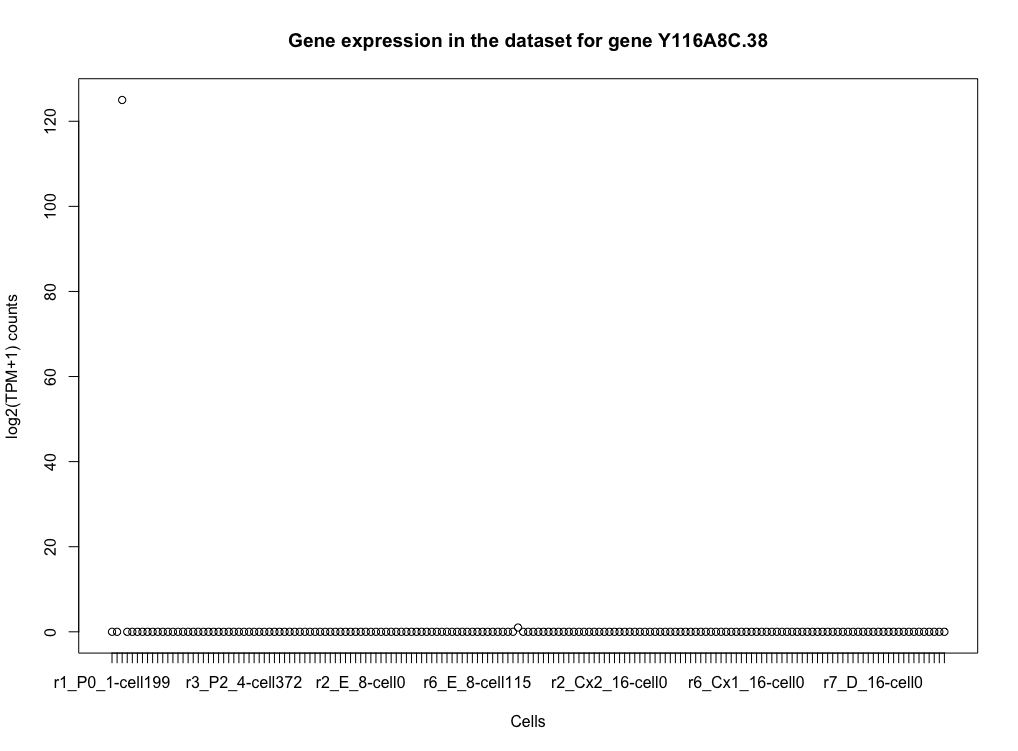
\includegraphics[scale=0.35]{plotsCopula/tintori/depCellGene_m=5_tintori_nodropout.png}
\subfigure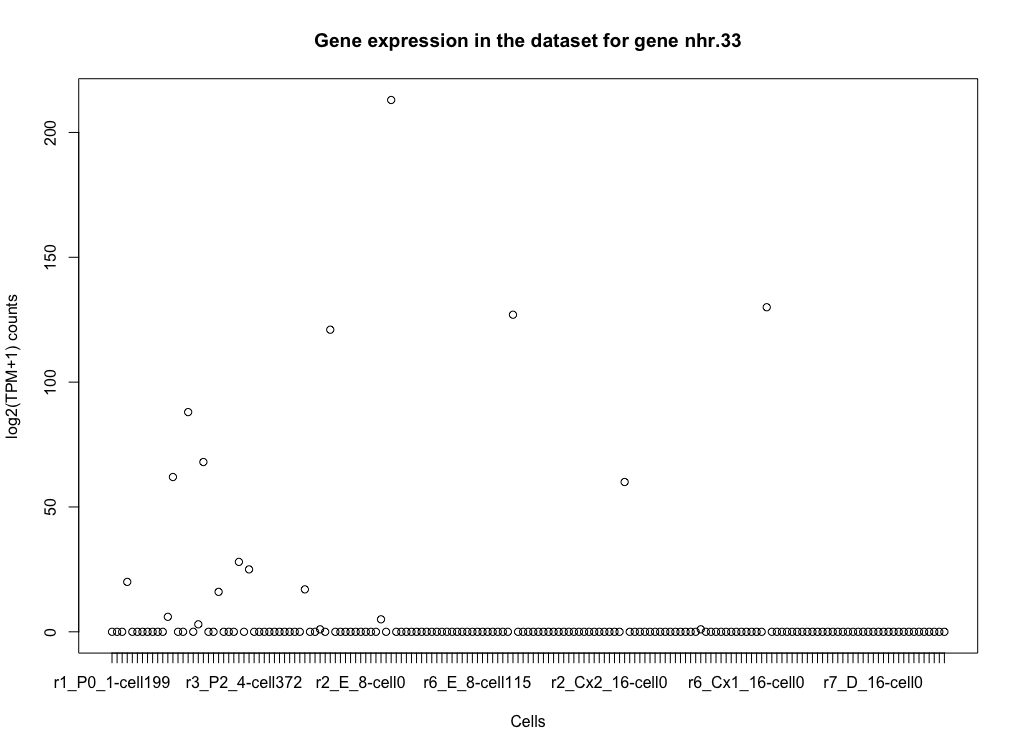
\includegraphics[scale=0.35]{plotsCopula/tintori/depCellGene_m=5_tintori_nodropout3.png}
\caption{Gene expression values for two non-dropout genes in the Tintori dataset (cells in $x$ axis, values in $y$ axis)}
\label{geneexpression1}
\end{figure}

\begin{figure}[H]
\centering
\subfigure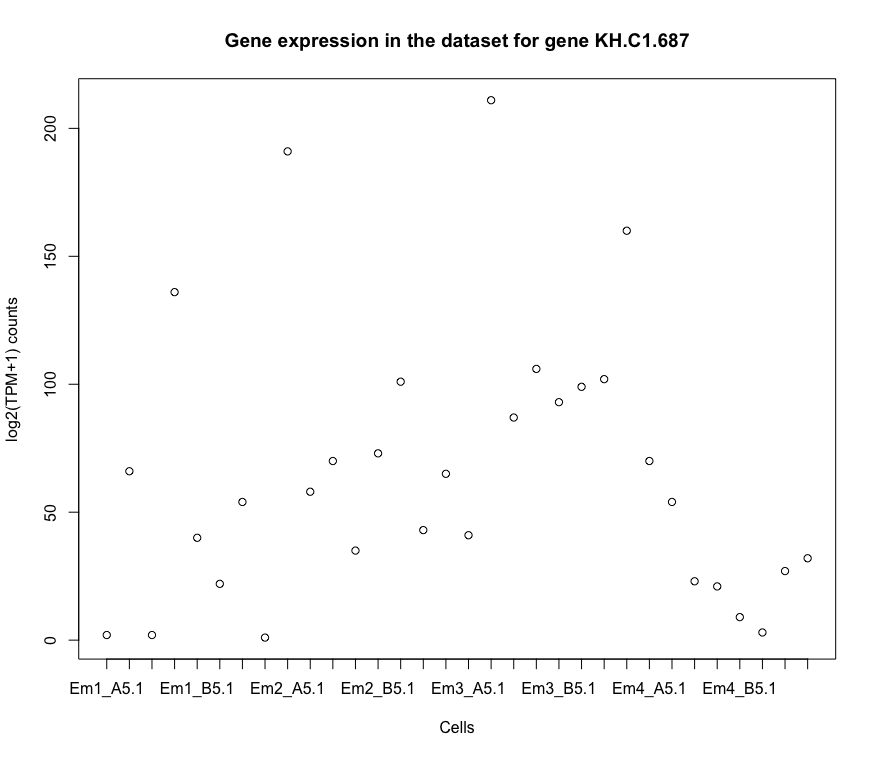
\includegraphics[scale=0.35]{plotsCopula/ciona/depCellGene_nodropout_ciona.png}
\subfigure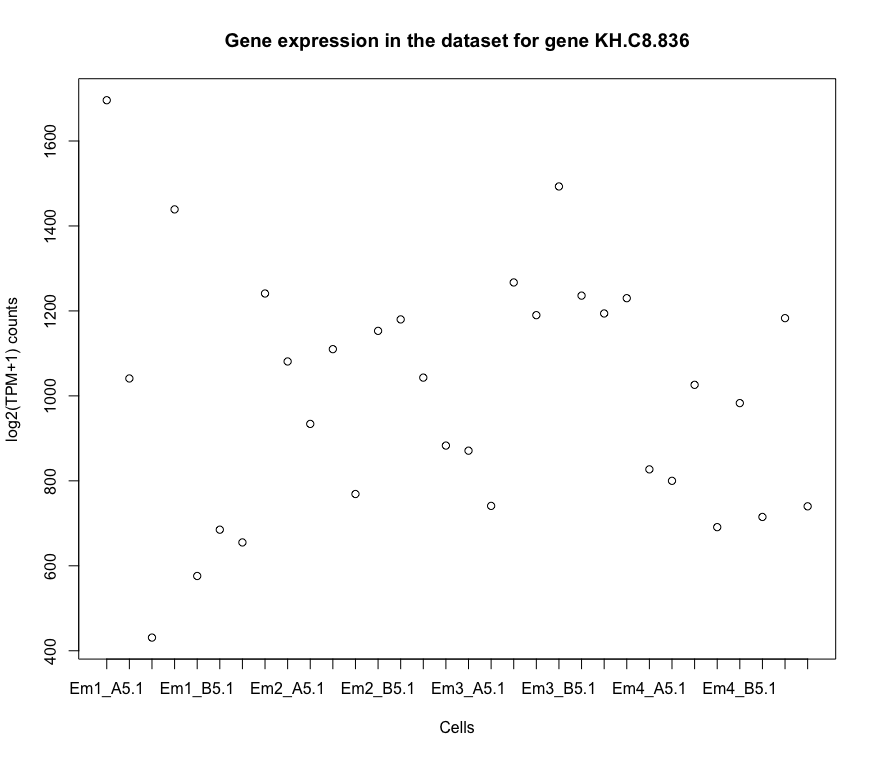
\includegraphics[scale=0.35]{plotsCopula/ciona/depCellGene2_nodropout_ciona.png}
\caption{Gene expression values for two non-dropout genes in the Ciona dataset (cells in $x$ axis, values in $y$ axis)}
\label{geneexpression2}
\end{figure}

\begin{figure}[H]
\centering
\subfigure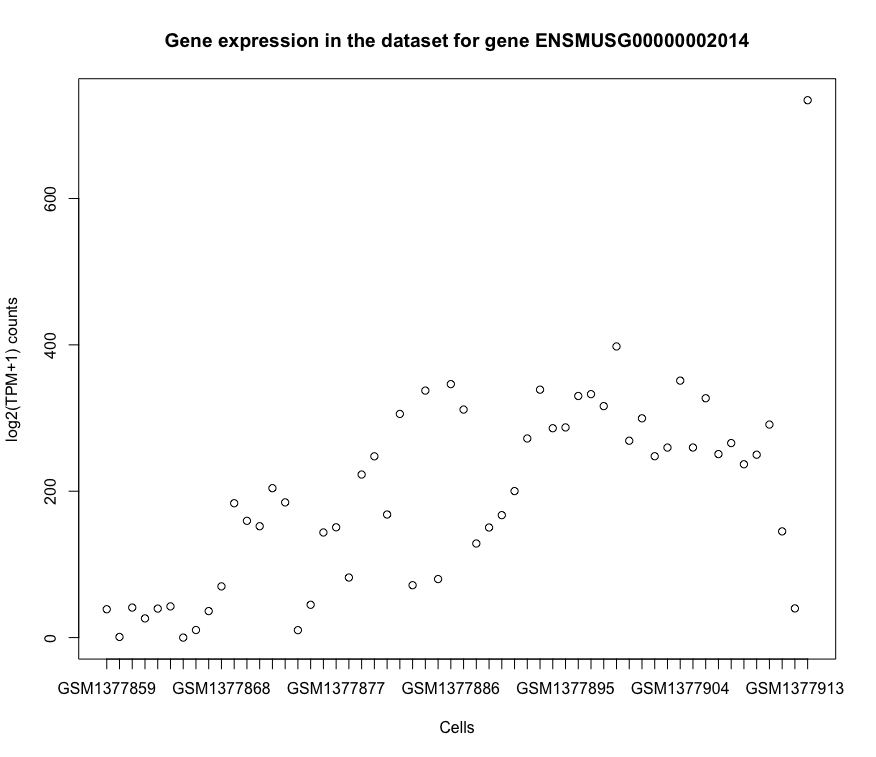
\includegraphics[scale=0.35]{plotsCopula/biase/depCellGene_nodropout_biase.png}
\subfigure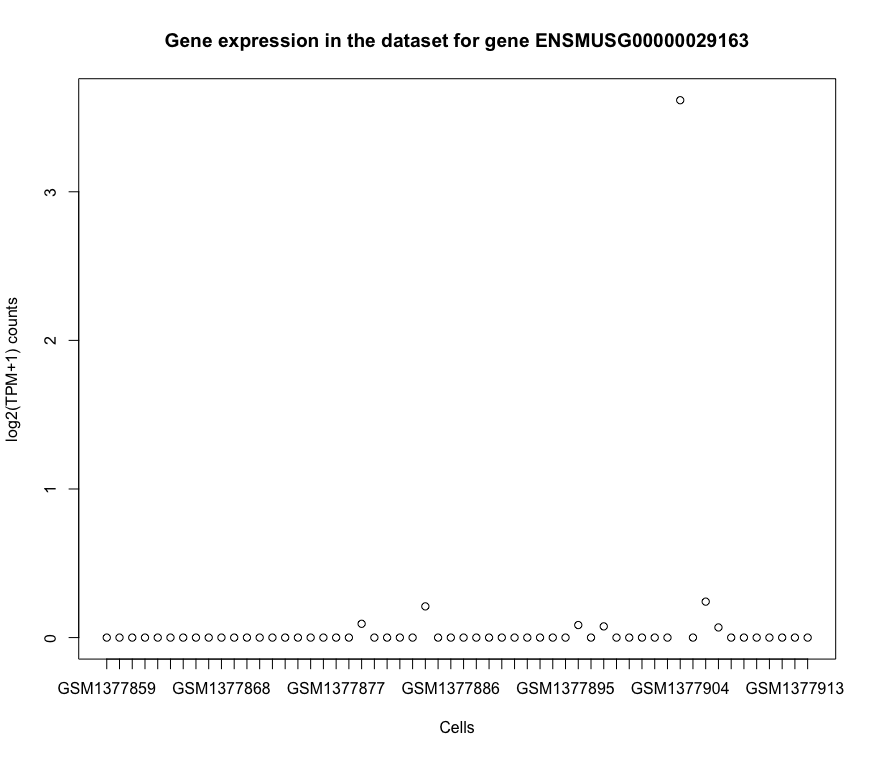
\includegraphics[scale=0.35]{plotsCopula/biase/depCellGene2_nodropout_biase.png}
\caption{Gene expression values for two non-dropout genes in the Biase dataset (cells in $x$ axis, values in $y$ axis)}
\label{geneexpression3}
\end{figure}

\section*{Copula distribution}

The following plots (produced by the function \textit{pairs.panels} from package \textbf{psych}) represent a histogram of the values found in each cell, the correlation ellipses found between two different cells, the linear model found (the red line) and the correlation number between the two vectors associated with the two cells of the considered pair. Missing values (NA) for dropout genes are due to the null variance of their gene expression values. More plots can be found at: {\url{https://github.com/oist-gene-clustering/mine}}\\

\begin{figure}[H]
\centering
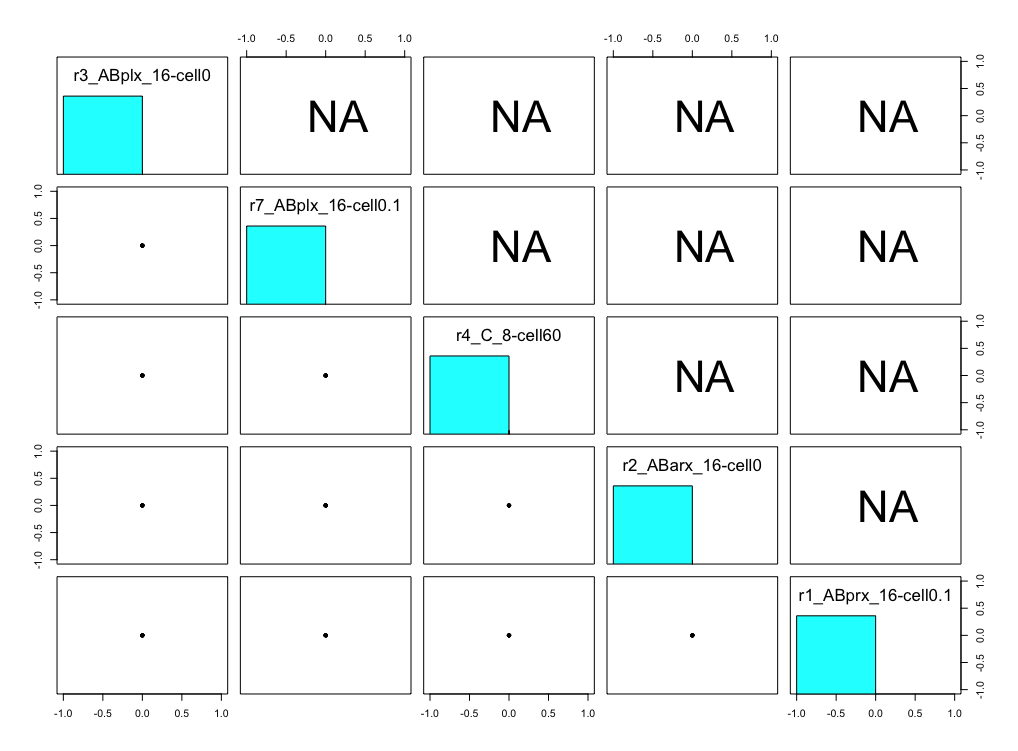
\includegraphics[scale=0.4]{plotsCopula/tintori/depCellnGene_dropout_tintori.png}
\caption{Correlation between $5$ cells (which names are written on the plot) from the Tintori dataset according to the gene expression in $5$ randomly-selected \textbf{dropout} genes}
\label{cellcorrelationdropout}
\end{figure}

\begin{figure}[H]
\centering
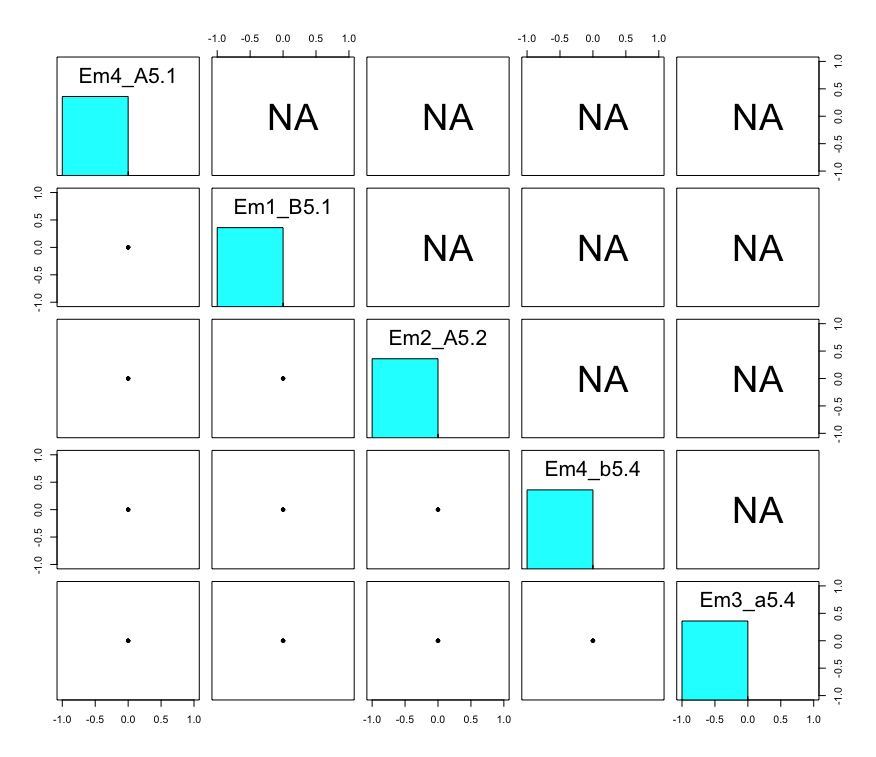
\includegraphics[scale=0.4]{plotsCopula/ciona/depCellnGene_dropout_ciona.png}
\caption{Correlation between $5$ cells (which names are written on the plot) from the Ciona dataset according to the gene expression in $5$ randomly-selected \textbf{dropout} genes}
\label{cellcorrelationdropout2}
\end{figure}

\begin{figure}[H]
\centering
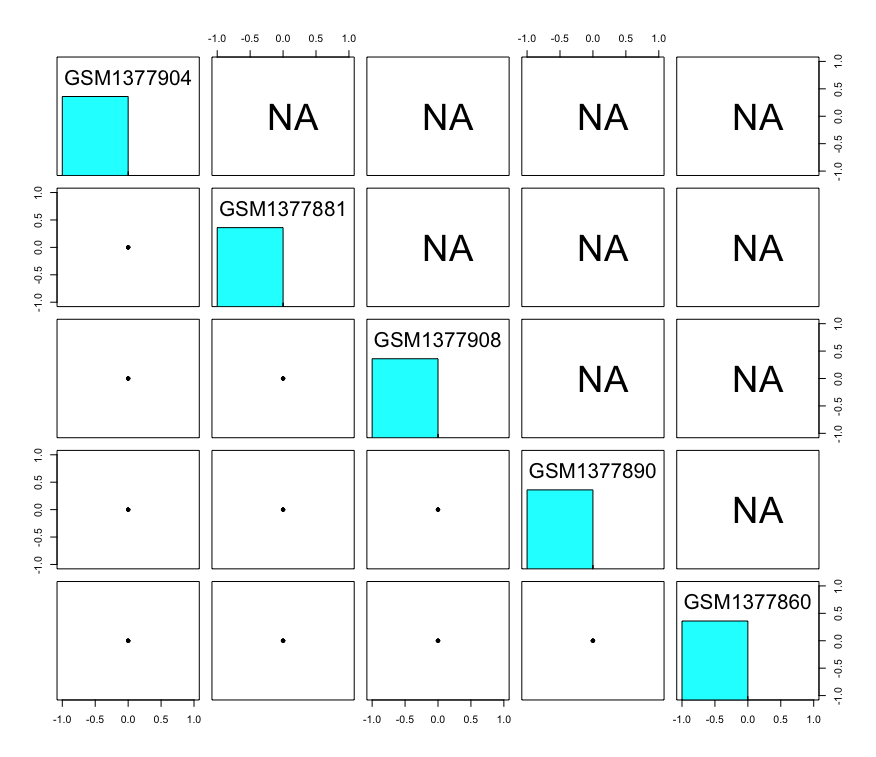
\includegraphics[scale=0.4]{plotsCopula/biase/depCellnGene_dropout_biase.png}
\caption{Correlation between $5$ cells (which names are written on the plot) from the Biase dataset according to the gene expression in $5$ randomly-selected \textbf{dropout} genes}
\label{cellcorrelationdropout3}
\end{figure}

\begin{figure}[H]
\centering
\subfigure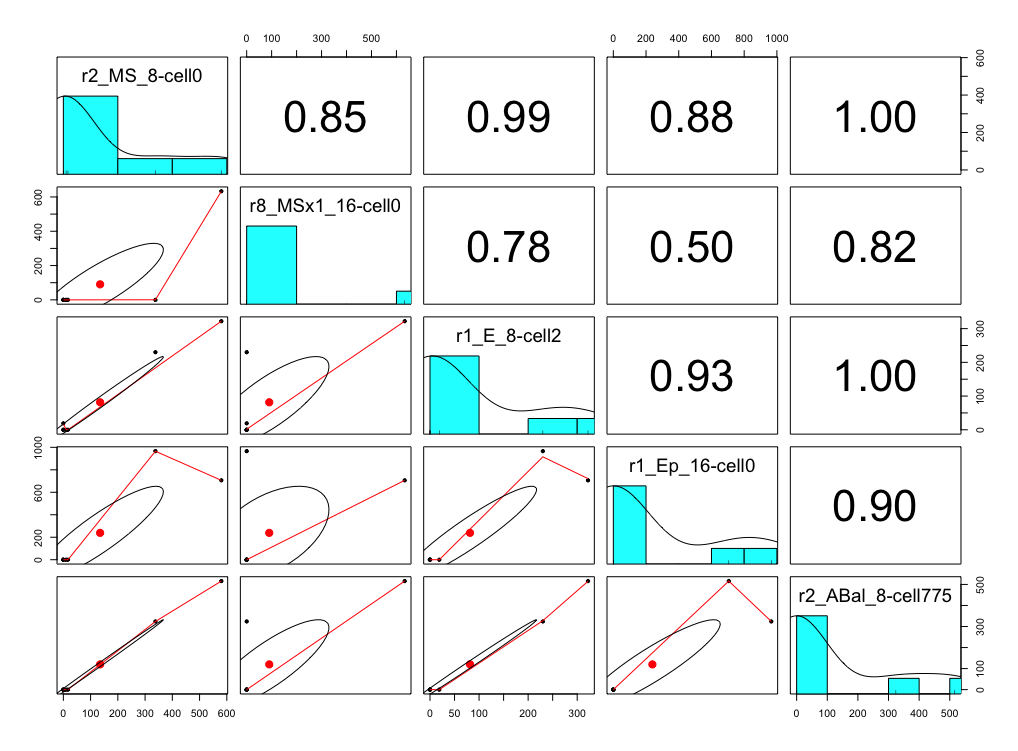
\includegraphics[scale=0.35]{plotsCopula/tintori/depCellnGene_nodropout_tintori.png}
\subfigure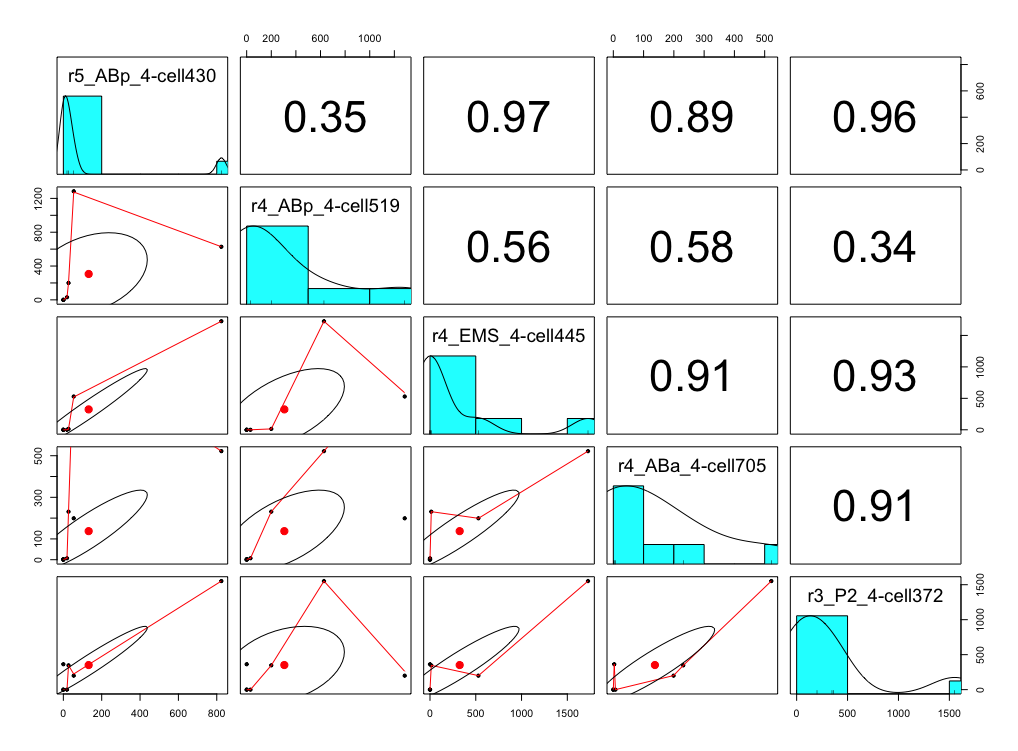
\includegraphics[scale=0.35]{plotsCopula/tintori/depCellnGene_nodropout_stage=4_tintori.png}
\caption{Correlation between $5$ cells (which names are written on the plot) from the Tintori dataset according to the gene expression in $5$ randomly-selected \textbf{non-dropout} genes (top). Correlation between $5$ 4-stage cells (which names are written on the plot) from the Tintori dataset according to the gene expression in $5$ randomly-selected \textbf{non-dropout} genes.}
\label{cellcorrelationnodropout}
\end{figure}

\begin{figure}[H]
\centering
\subfigure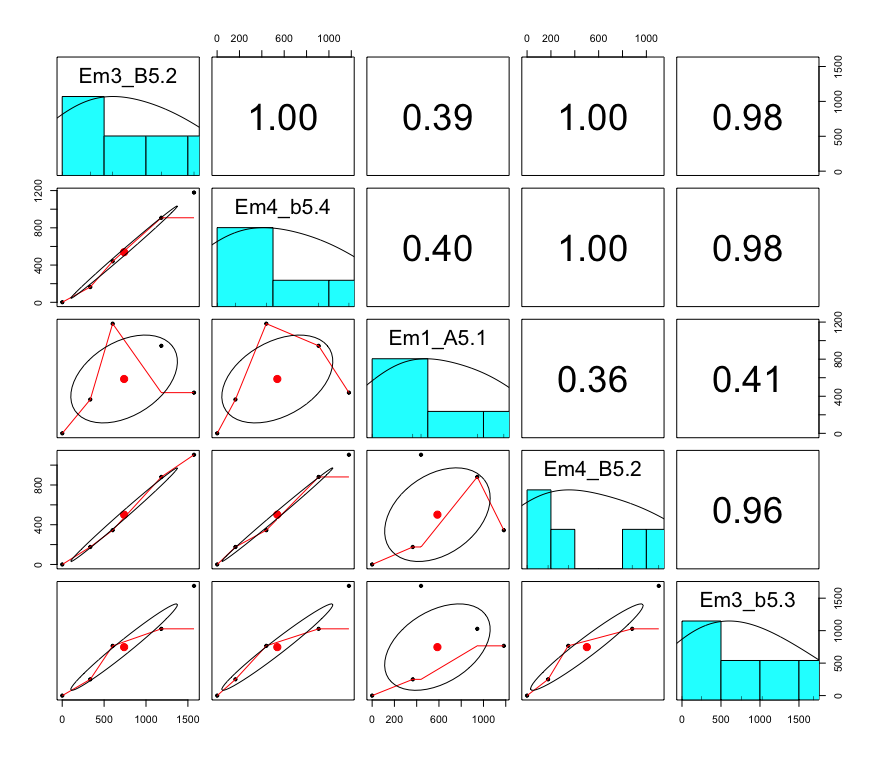
\includegraphics[scale=0.35]{plotsCopula/ciona/depCellnGene_nodropout_ciona.png}
\subfigure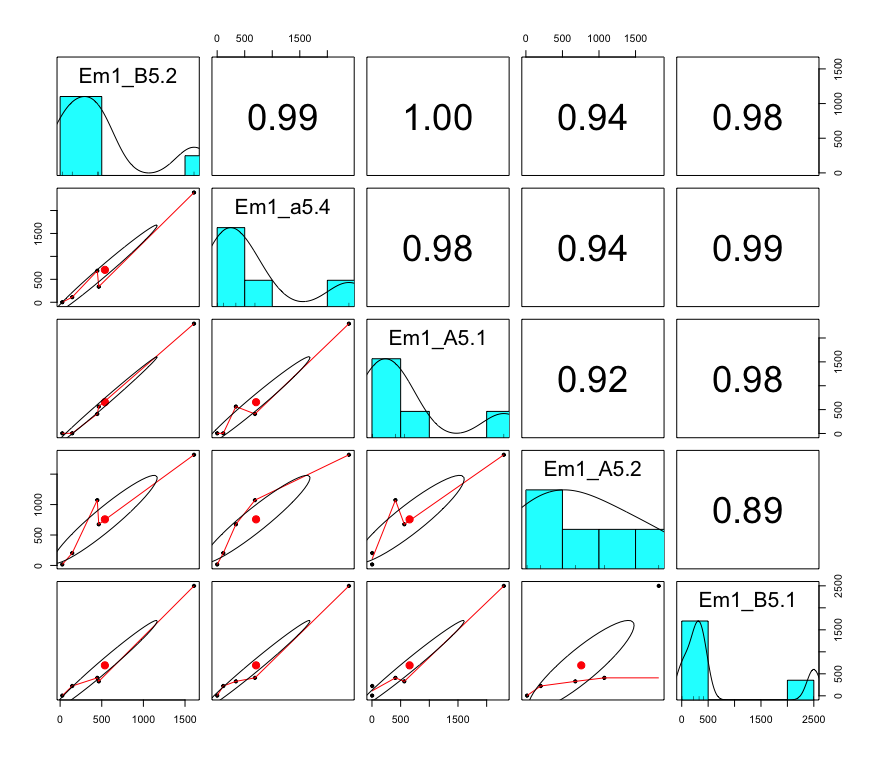
\includegraphics[scale=0.35]{plotsCopula/ciona/depCellnGene_nodropout_em1_ciona.png}
\caption{Correlation between $5$ cells (which names are written on the plot) from the Ciona dataset according to the gene expression in $5$ randomly-selected \textbf{non-dropout} genes (top). Correlation between $5$ cells from Embryo 1 (which names are written on the plot) from the Ciona dataset according to the gene expression in $5$ randomly-selected \textbf{non-dropout} genes.}
\label{cellcorrelationnodropout2}
\end{figure}

%% plots pour les copulas et relation entre variables et latent variables

It can noticed that cells from a same embryo are highly correlated, even if they have different cell types.

\section*{Parameter estimation methods}

Four sets of parameters need to be estimated: the Poisson-like distribution parameter, the Negative Binomial-like mean and dispersion parameters, the mixture rates for margin and copula distributions, and the copula parameters, that is, the two means of the bimodal copula and the covariance matrix parameter. I used for each of these parameters a non-optimization method, to lessen the computational cost of the algorithm, and to ensure more accuracy and more stability.

\bigskip
\noindent \textit{Poisson-like parameter}
\bigskip

As explained in the previous section, this parameter is set to an arbitrary constant, which is the same as the one used by \cite{kharchenko2014bayesian}: $\lambda_0 = 0.1$.

\bigskip
\noindent \textit{Negative Binomial-like parameters}
\bigskip

The mean is found by the method for DESeq2 software, first described by \cite{anders2010differential}, which formula is displayed in the \textbf{Modeling} section. The dispersion parameter is found by the shrinkage estimation method described in \cite{yu2013shrinkage}.

\bigskip
\noindent \textit{Mixture rate parameters}
\bigskip

I assumed that the dropout events (resp. mild-high expressiveness events) of different (sets of) genes are independent, thus a logistic regression can be applied to predict the probability of the considered event\cite{andersonLogistic}\cite{petersLecture}\cite{frostWhy}.\\

%[TODO ADD PLOTS]\\

\begin{itemize}
\item After application of the MAST function, gene expression values of genes which are considered dropout (i.e. which gene expression value is thought to be background noise) are set to zero.\\

Actually, \cite{finak2015mast} shows the choice of the background noise value does not matter much. I can thus later annotate genes being dropout by marking genes having a null expression value. Dropout events are considered to depend on the mean gene expression value of a feature\cite{kharchenko2014bayesian}. However, the absolute value of a gene in a given cell by itself is not useful, the most important part is to know the gene expression value respect to the expression values of other genes in the same cell.\\

Hence the values on which the regression will be performed are the following weighted mean values: if C is the set of cells, and G the set of genes, the value associated with a given gene $g$ is: $\sum{_{j \in C} \frac{M[g, j]}{\sum{_{k \in G} M[k, j]}}}$.
\item The MAST function also computes the "activation" gene expression threshold, such as, if the expression value of a given gene is above this threshold, then this gene is considered highly-expressed, mildly-expressed otherwise. This threshold is the valley -when it exists- between the two peaks in gene expression density, that is, what I see as the two nodes of the bimodal gene expression.
\end{itemize}

\begin{figure}[H]
\centering
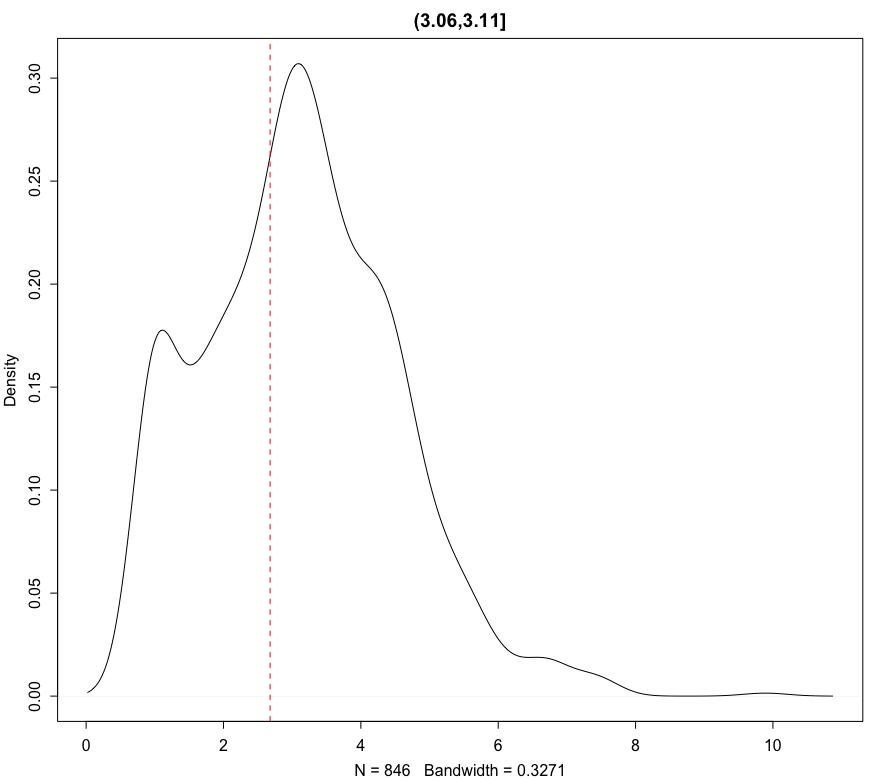
\includegraphics[scale=0.35]{illustrations/densityCionaLogNorm.png}
\caption{Result of kernel density estimation\cite{parzen1962estimation} (on n=846 points) applied on log-normalized gene expression values (that belong to the interval (3.06,3.11]) from the Ciona\cite{suyama2016singlecell} scRNAseq dataset. Kernel estimation is a method used to estimate the density function of a random variable (here, the expression value of a gene in a given cell) from a sample. The red vertical line is the threshold found by the MAST package.}
\label{densityCiona2}
\end{figure}

\bigskip
\noindent \textit{Copula parameters}
\bigskip

For a given copula, the mean vectors of the bimodal Gaussian copula are the two highest peaks in the kernel density estimation performed by MAST. The covariance matrix is estimated via the corpcor R package\cite{schafer2005shrinkage}.

\section*{Clustering algorithm}

\bigskip
\noindent \textbf{Pre-processing (pre-processing step in cluster analysis)}
\bigskip

\begin{itemize}
\item For a given positive integer $k$, $M[k,]$ is the $k$th row of M, and for $i,j$ positive integers, $M[i,j]$ is the coefficient in $i$th row and $j$th column of M.
\item TPM (\textit{Transcripts Per Kilobase Million}) is one of the most common normalization methods used for scRNA-seq (see \cite{normMethods} for a review of the different methods). Indeed, as a general rule, the total gene expression count over all the detected genes varies from one cell to another, thus making the raw counts not directly comparable between cells. Also, the length of the coding sequence may change from one gene to another. In order to compare gene expression values of different features in a given sample, counts should also be normalized to take this into account\cite{love2014moderated}. 
\item Feature selection is an unavoidable step in clustering\cite{liu2006efficient}. I use a quick and intuitive \textit{ad hoc} method, which is similar to \cite{kuhn2008caret}. Given my definition of informative genes (see \textbf{Modeling} section), I choose a threshold of correlation $d'$, such as if two genes have an absolute correlation value above this threshold, and if they have roughly a similar mean expression value, they are considered truly correlated. Note that the condition on the mean expression values should not be ignored, see \cite{guyon2003introduction} for example. Then I compute a distance based on these two conditions on the set of genes, and apply hierarchical clustering on the resulting distance matrix, Then I cut the obtained dendrogram at height $1-d'$, (see Figure \ref{treecut}) and keep only one gene of each of the resulting clusters. I chose Spearman's $\rho$ for the correlation function, and an \textit{average-linkage} strategy for the clustering, according to the benchmark performed by \cite{jaskowiak2014selection}.
\item Null variance rows/features are deleted, for they are non informative of expression changes across the samples
\item Rows are also trimmed according to the frequency of expression of a given gene across the set of conditions. If a gene is ubiquitous, it will not be helpful in order to determine the differences between conditions\cite{guo2015sincera}\cite{kiselev2016sc3}.
\end{itemize}

\begin{algorithm}[H]
\caption{Function \emph{filter}}
\begin{algorithmic}
\STATE \textbf{Input}: M, gene expression matrix of size $p \times m$
\STATE \textbf{Output}: filtered gene expression matrix
\STATE Remove rows with missing values
\STATE Remove null-variance rows
\IF {M is already normalized} 
\STATE $\forall i \leq p, \forall j \leq m$, $M_{i,j} \leftarrow$ $\frac{1}{log(2)} \times log(M_{i,j}+1)$
\ELSE 
\STATE $\forall i \leq p, \forall j \leq m$, $M_{i,j} \leftarrow$ $\frac{1}{log(2)} \times log(\frac{M_{i,j}}{\sum{_{k \leq p} M_{k,j}}} \times 10^6+1)$
\ENDIF
\RETURN{M}
\end{algorithmic}
\end{algorithm}

\begin{algorithm}[H]
\caption{Function \emph{featureSelect}}
\begin{algorithmic}
\STATE \textbf{Input}: M, gene expression matrix of size $p \times m$
\STATE \textbf{(hidden) parameter}: $d'$, threshold of correlation between features 
\STATE \textbf{Output}: gene expression matrix with trimmed rows
\STATE dMatrix $\leftarrow$ \textbf{NULL}
\STATE $\forall i \leq p, \forall k \leq p$, dMatrix[i,k] $\leftarrow 1-correlation(M[i,], M[k,])$
\STATE Apply hierarchical clustering to the row vectors of M using dmatrix
\STATE Cut the hierarchical tree at height $1-d'$
\STATE selectedFeatures $\leftarrow$ clusters from the cut tree
\STATE Remove from M rows NOT appearing in selectedFeatures
\RETURN{M}
\end{algorithmic}
\end{algorithm}

\begin{figure}[H]
\centering
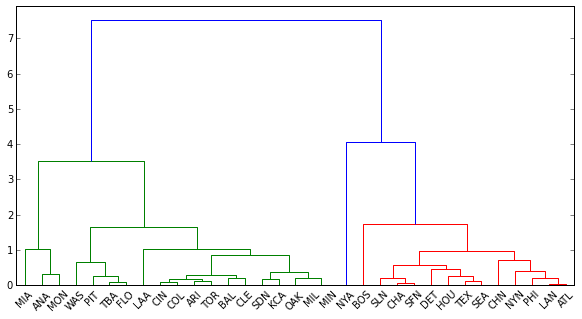
\includegraphics[scale=0.5]{illustrations/treecut.png}
\caption{Example of tree resulting from a hierarchical clustering of the data\cite{imgTreecut}. The leaves are the clustered elements, and the more the two groups at a given node are similar, the shorter the branches are. If this tree is cut at height 3 (y axis), then there are 4 clusters. If it is cut at height 5, there are two resulting clusters.}
\label{treecut}
\end{figure}

\begin{algorithm}[H]
\caption{Function \emph{frequenceTrim}}
\begin{algorithmic}
\STATE \textbf{Input}: M, gene expression matrix of size $p \times m$
\STATE \textbf{(hidden) parameter}: $f$, maximum feature frequency allowed in data
\STATE \textbf{Output}: trimmed gene expression matrix
\STATE Remove in M features present in more than $f \times 100 \%$ of the conditions
\RETURN{M}
\end{algorithmic}
\end{algorithm}

\bigskip
\noindent \textbf{Find the most probable patterns (pre-processing step)}
\bigskip

The idea behind this step is:

\begin{enumerate}
\item to classify genes into dropout/non-dropout genes.
\item to find the \textbf{activation threshold} for every gene in each cell, that is, if the expression value of a certain gene in a certain cell type is above the so-called activation threshold associated with this gene and this condition, it means that this gene is activated -also called \textbf{highly-expressed}- in this cell. Otherwise, the gene is considered \textbf{mildly-expressed}. 
\item to fit logistic models for dropout and mild/high gene expressiveness events for a given gene, in a given cell.
\end{enumerate}

The \textit{thresholdComputation} function is the \textit{thresholdSCRNACountMatrix} function from MAST R package (described in \cite{finak2015mast}), which determines adaptively the gene expression value threshold $t$ (using kernel density estimation) such as, if the expression value associated with one gene is below $t$, then the gene is considered dropout, and its expression value is replaced by a constant value corresponding to background noise (arbitrarily fixed at zero, see \cite{finak2015mast} for details). It also computes one of the lowest valley points between the two modes of gene expression, which is considered the \textbf{activation threshold} (see Figure \ref{densityCiona2}).\\

\begin{algorithm}[H]
\caption{Finding pattern part (function \emph{getPatterns})}
\begin{algorithmic}
\STATE \textbf{Input}: M, new dropout-thresholded gene expression matrix of size $p \times m$, and \textit{res}, result of the \textit{thresholdComputation} function
\STATE \textbf{Output}: modelDropout and modelMild, logistic models, and P, matrix of cell patterns, Q, pattern-oriented matrix
\FOR {$i \leq p$}
\IF{$\sum{_{k \leq p} M[k, j]} = 0$}
\STATE $v \leftarrow 0$
\ELSE
\STATE $v \leftarrow \sum{_{j \leq m} \frac{M[i,j]}{\sum{_{k \leq p} M[k, j]}}}$
\ENDIF
\IF{$v = 0$}
\STATE Mark gene $i$ as dropout
\ELSE
\STATE Mark gene $i$ as non-dropout
\ENDIF
\ENDFOR
\STATE thresholds $\leftarrow$ list of threshold values in res (vector of length $m$)
\FOR{$j \leq m$}
\FOR{$i \leq p$}
\IF{$M[i,j] \leq $ threshold[$j$]}
\STATE Mark gene $i$ in cell $j$ as mildly-expressed
\ELSE
\STATE Mark gene $i$ in cell $j$ as highly-expressed
\ENDIF
\ENDFOR
\ENDFOR
\STATE modelDropout $\leftarrow$ logistic regression using $k$-fold cross validation 
\STATE modelMild $\leftarrow$ logistic regression using $k$-fold cross validation for each condition
\STATE $P \leftarrow$ \textbf{NULL}
\STATE $Q \leftarrow$ \textbf{NULL}
\FOR{$j \leq m$}
\FOR{$i \leq p$}
\IF{gene $i$ in cell $j$ marked as mildly-expressed}
\STATE $P[i,j] \leftarrow 0$
\STATE $Q[i,j] \leftarrow$ threshold[$j$]
\ELSE
\STATE $P[i,j] \leftarrow 1$
\STATE $Q[i,j] \leftarrow$ -threshold[$j$]
\ENDIF
\ENDFOR
\ENDFOR
\RETURN{modelDropout, modelMild, P, Q}
\end{algorithmic}
\end{algorithm}

\bigskip
\noindent \textbf{Computation of the gene expression distribution for each cell (pre-processing step)}
\bigskip

The objectives of this part of the algorithm are:
\begin{enumerate}
\item to find the best estimates for the margin parameters.
\item to find the best estimates for the mixtures rates.
\item to find the best estimates for the copula parameters.
\end{enumerate}

The \textif{estimateMarginParameters} function uses formulas for mean and dispersion parameter estimation from respectively \cite{anders2010differential} and \cite{yu2013shrinkage}. The formula for the mean parameter is recalled below (M being the gene expression matrix):

\begin{definition}[Size factor]\label{sizefactor}{For cell $j$:\begin{center}sizeFactors[$j$] = \textit{median}$_{i \leq p} \frac{M[i, j]}{\prod_{l \leq m} (M[i, k]+1)^{(\frac{1}{m})}}$\end{center}}\end{definition}

\begin{definition}[Estimated gene expression mean]\label{marginmean}{For gene $i$:\begin{center}margin\_means[$i$] = $\sum{_{j \leq m} \frac{M[i, j]}{m \times sizeFactors[j]}}$\end{center}}\end{definition}

The estimated gene expression dispersion vectors margin\_deltas are obtained by the shrinkage estimation method described in \cite{yu2013shrinkage}.\\

The correlation matrix is found by the method described in \cite{schafer2005shrinkage}, which allows to find a target correlation matrix T such as T is diagonal: $\exists \nu \in (\mathbb{R}^{+})^{p}, T = $\textit{diag}$(\nu)$, which allows for different variances. This is a commonly used model for gene expression covariance matrices, although it is really restrictive, and it is unsure whether it can actually describe properly the true gene regulatory system. This computation is provided by the R package \textbf{corpcor}. I could have used the formula suggested by \cite{chen2009shrinkage}, as it is especially targeted at Gaussian distributions, but the resulting matrix is $\beta \times I_d$, where $I_d$ is the identity matrix and $\beta \in \mathbb{R}^{+}$, which is a even more constrained model. Optimization methods often fail, because the quadratic system to solve is often singular, due to the large number of zeroes in the gene expression matrix, and when it actually works, the resulting matrix is often ill-conditioned -even when a regularization is applied to the optimization problem- so not only not useful in practice, but also probably wrong biologically speaking.

%%The two mean vector parameters for the bimodal copulas are defined as follows: for a given copula/condition and a given gene, 

The mixture rate for margin and copula functions are computed with the logistic regression models fitted as described above.

\bigskip
\noindent \textbf{Merge pattern clusters (pre-processing step)}
\bigskip

The idea behind this is to obtain a list of pairs of cell types, ordered by decreasing similarity value, that are similar "enough" (in the sense of the cell similarity definition given previously), that I call "mergeable pairs". The function \emph{computeSimilarity} is the implementation of the measure $sim$. \emph{distMatrix} is the distance matrix deduced from the similarity values.\\

\bigskip
\noindent \textbf{Clustering (clustering step)}
\bigskip

The strategy for merging cell clusters is close to the K-Nearest Neighbor strategy. The main idea is to consider mergeable pairs in decreasing similarity value order, and, if the two elements of the pair are in different clusters, see if there are K points in the same cluster of one of the elements that are similar "enough" to the other element (\textit{K neighbors agreeing to the merging}), and vice-versa, and, if this condition is satisfied, then merge the clusters.\\

\begin{definition}[Neighbor in a cluster]\label{neighbor}{The set of neighbors of a point $k$ in a given cluster is the set of all points, different from $k$, that belong to this cluster.}\end{definition}

\begin{definition}[Neighbor agreement]\label{neighboragreement}{Let $d$ be a probability threshold ($d \geq 0.5$). A neighbor of a point $k$ agrees with the merging of its cluster and a distinct cluster of a point $l$ iff. $sim(k,l) > d$.}\end{definition}

\begin{definition}[Same-cluster neighbor agreement]\label{neighborsagreement}{Let K be a nonzero integer. K neighbors of a point $k$ agree with the merging of their cluster and a distinct cluster of a point $l$ iff. there are K neighbors of $k$ which agree with the merging.}\end{definition}

\begin{definition}[Condition for the merging of clusters]\label{mergingclusters}{Let K be a nonzero integer. Two clusters can be merged (via a mergeable pair ($k$, $l$)) iff. K neighbors of $k$ and K neighbors of $l$ agree with the merging.}\end{definition}

At first, clusters are initialized to $m$ clusters, containing only one condition each.\\

K controls the granularity of the clustering algorithm: the more K is big, the more it will be hard to merge two clusters. Furthermore, I chose to have the number of neighbors K needed for agreement specific to one cluster, and change according to the size of this cluster. I want to make the merging of two small clusters easier, and conversely, the merging of a bigger cluster harder, because smaller clusters are most likely more homogenous than big ones, and I want to keep the clusters balanced respect to the correlation between all points in a same cluster. A "good choice" for the K-Nearest Neighbor strategy (with Euclidian distance) is actually having $K \thicksim \sqrt{n}$, where $n$ is the total number of elements (see Stone's theorem\cite{stone1977consistent}). Although the underlying "distance" used in the merging of the clusters is \textbf{not} an Euclidean distance (because it is not a distance...), this strategy seems to suit the behavior I would like to see for the cluster merging, even though it is not asserted by a consistency theorem.\\

Henceforth, in my algorithm, at a given iteration $i$ of the inner loop, for a given cluster $C_i$, the number of neighbors needed for agreement $K_{C_i}$ is $\floor{\sqrt{\#C_i-1}}$ (because my definition of neighbor does not include the considered node itself).\\

\bigskip
\noindent \textbf{Measures (Validation step)}
\bigskip

In the future, the user would be able to get access to the error rate for the logistic regressions, and on the estimates for the margin and copula parameters.

\chapter{Benchmark}

\section*{Ranking}

Let A denote the set of algorithms, and D the set of test datasets. Since the datasets have been produced with different methods, and are of variable quality, I decided to take into account the mean performance of all algorithms on a given dataset for the final ranking.\\

For each quantity $q$ (that gives the value of the corresponding attribute: \textit{time}, \textit{accuracy}, ... for a given dataset and a given algorithm) listed in the columns of the next table (except for \textit{time}), I used the following score function and weights:

\begin{definition}[Overall performance on a dataset]\label{performancedataset}{For a dataset $d$: 

\begin{center}$\rho_{d} = $median$_{a \in A}$(accuracy$(d, a))$\end{center}}\end{definition}

\begin{definition}[Weight associated with a dataset]\label{weightdataset}{For a dataset $d$: \begin{center}$\delta_{d} = \frac{\rho_{d}}{\sum{_{d' \in D} \rho_{d'}}$\end{center}}\end{definition}

Thus this function gives more weight to results from datasets on which the tested algorithms give their best outputs, because these datasets are considered more relevant than other datasets where the clustering pattern is less easy to find.

\begin{definition}[Score function]\label{scorefunction}{For an algorithm $a$, evaluated for a given quantity $q$: \begin{center}score$_{q, d}$($a$) = $\sum{_{d \in D}$ $\rho_{d} \times q(d, a)$}\end{center}}\end{definition}

The ranking for an algorithm and a given quantity is the position of the corresponding score in the ordered vector of scores for all algorithms. For the ranking, I only took into account the results from all datasets except for Treutlein, Ciona, Klein and Usoskin, because I could not get results for the NMF and SNN-Cliq algorithms on these datasets (see next section).

\section*{Test datasets}

The datasets have been formatted by \cite{datasetsSource}. Using the classification suggested by \cite{kiselev2016sc3}, I sorted the datasets into \textbf{gold standard} and \textbf{silver standard} datasets, that is, the clustering described in the corresponding article for gold standard datasets has been found or confirmed by biological means, and not by computation or clustering. This information allows to better interpret the number of clusters found by the different algorithms: the clusterings found for gold standard datasets are expected to be less biased than the silver standard ones.\\ 

Table \ref{datasets} displays the following info about the test datasets:

\begin{itemize}
\item the organism from which the biological data comes from.
\item whether the considered dataset is gold or silver standard.
\item the expected number of clusters, and the number of clusters for the "reference" clustering.
\item the dimensions of the gene expression matrix, that is, the number of features times the number of conditions.
\end{itemize}

\begin{table}[H]
\centering
\caption{Test datasets for the benchmark}
\begin{tabular}{| c | c | c | c | c | c |}
\hline
\parbox[c]{3cm}{\textbf{Dataset}} & 
\parbox[c]{2cm}{\textbf{Organism}} & 
\parbox[c]{3cm}{\textbf{Date /\\Technology}} & 
\parbox[c]{2cm}{\textbf{Standard}} &
\parbox[c]{2cm}{\textbf{Exp. | Ref.}}&
\parbox[c]{2cm}{\textbf{Dimensions}}\\
\hline
\parbox[c]{3cm}{Biase\cite{biase2014cell}} & 
\parbox[c]{2cm}{Mouse} & 
\parbox[c]{3cm}{2014 /\\SMARTer} & 
\parbox[c]{2cm}{Gold} &
\parbox[c]{2cm}{5 | 6}&
\parbox[c]{2cm}{$25,737 \times 56$}\\
\hline
\parbox[c]{3cm}{Ciona\cite{suyama2016singlecell}}& 
\parbox[c]{2cm}{Ciona}& 
\parbox[c]{3cm}{2014 /\\Tang} & 
\parbox[c]{2cm}{Gold}&
\parbox[c]{2cm}{5 | 5}&
\parbox[c]{2cm}{$15,288 \times 32$}\\
\hline
\parbox[c]{3cm}{Deng\cite{deng2014single}}& 
\parbox[c]{2cm}{Mouse}& 
\parbox[c]{2cm}{2014 /\\SMARTSeq} & 
\parbox[c]{2cm}{Gold}&
\parbox[c]{2cm}{9 | 10}&
\parbox[c]{2cm}{$22,958 \times 317$}\\
\hline
\parbox[c]{3cm}{Goolam\cite{goolam2016heterogeneity}} & 
\parbox[c]{2cm}{Mouse} & 
\parbox[c]{3cm}{2016 /\\SMARTSeq2} & 
\parbox[c]{2cm}{Gold} &
\parbox[c]{2cm}{8 | 5}&
\parbox[c]{2cm}{$41,388 \times 124$}\\
\hline
\parbox[c]{3cm}{Kolodziejczyk\cite{kolodziejczyk2015single}} & 
\parbox[c]{2cm}{Mouse} & 
\parbox[c]{3cm}{2015 /\\Wellcome Trust Sanger} & 
\parbox[c]{2cm}{Gold}&
\parbox[c]{2cm}{11 | 9}&
\parbox[c]{2cm}{$38,653 \times 704$}\\
\hline
\parbox[c]{3cm}{Tintori\cite{tintori2016transcriptional}}& 
\parbox[c]{2cm}{C. elegans}& 
\parbox[c]{3cm}{2016 /\\SMARTer} & 
\parbox[c]{2cm}{Gold}&
\parbox[c]{2cm}{5 | 5}&
\parbox[c]{2cm}{$31,383 \times 299$}\\
\hline
\parbox[c]{3cm}{Yan\cite{yan2013single}}& 
\parbox[c]{2cm}{Human} & 
\parbox[c]{3cm}{2013 /\\Tang} & 
\parbox[c]{2cm}{Gold} &
\parbox[c]{2cm}{7 | 7}&
\parbox[c]{2cm}{$20,214 \times 90$}\\
\hline
\parbox[c]{3cm}{Klein\cite{klein2015droplet}} & 
\parbox[c]{2cm}{Mouse} & 
\parbox[c]{3cm}{2015 /\\Droplet} & 
\parbox[c]{2cm}{Silver}&
\parbox[c]{2cm}{16 | 4}&
\parbox[c]{2cm}{$24,175 \times 2,717$}\\
\hline
\parbox[c]{3cm}{Treutlein\cite{treutlein2014reconstructing}} & 
\parbox[c]{2cm}{Mouse} & 
\parbox[c]{3cm}{2014 /\\SMARTer} & 
\parbox[c]{2cm}{Silver} &
\parbox[c]{2cm}{12 | 5}&
\parbox[c]{2cm}{$23,745 \times 196$}\\
\hline
\parbox[c]{3cm}{Usoskin\cite{usoskin2015unbiased}} & 
\parbox[c]{2cm}{Mouse} & 
\parbox[c]{3cm}{2015 /\\Islam} & 
\parbox[c]{2cm}{Silver} &
\parbox[c]{2cm}{15 | 11}&
\parbox[c]{2cm}{$25,334 \times 622$}\\
\hline
\end{tabular}
\label{datasets}
\end{table}

\section*{Details about the accuracy test performed}

\begin{table}[H]
\centering
\caption{ARI value (respect to the reference labels) and number of clusters found by each algorithm in datasets Biase, Ciona, Deng, Goolam and Kolodziejczyk (1)}
\begin{tabular}{| l | l | l | l | l |}
\hline
\parbox[c]{5cm}{\textbf{Dataset (Expected no.)\\ / Algorithm}} & 
\parbox[c]{2cm}{\textbf{SC3}} & 
\parbox[c]{2cm}{\textbf{PCAReduce}} &
\parbox[c]{2cm}{\textbf{K-means}}&
\parbox[c]{2cm}{\textbf{tSNE\\+DBSCAN}}\\
\hline
\parbox[c]{5cm}{\textbf{Biase (6)}} & 
\parbox[c]{2cm}{0.79 | 6} & 
\parbox[c]{2cm}{0.98 | 7} &
\parbox[c]{2cm}{0.99 | 6}&
\parbox[c]{2cm}{0.68 | 4}\\
\hline
\parbox[c]{5cm}{\textbf{Ciona (5)}} & 
\parbox[c]{2cm}{-0.11 | 5} & 
\parbox[c]{2cm}{-0.07 | 6} &
\parbox[c]{2cm}{-0.04 | 5}&
\parbox[c]{2cm}{0.01 | 2}\\
\hline
\parbox[c]{5cm}{\textbf{Deng (9)}} & 
\parbox[c]{2cm}{0.44 | 9} & 
\parbox[c]{2cm}{0.48 | 9} &
\parbox[c]{2cm}{0.00 | 9}&
\parbox[c]{2cm}{0.65 | 7}\\
\hline
\parbox[c]{5cm}{\textbf{Goolam (8)}} & 
\parbox[c]{2cm}{0.40 | 8} & 
\parbox[c]{2cm}{0.58 | 9} &
\parbox[c]{2cm}{0.89 | 8}&
\parbox[c]{2cm}{0.06 | 7}\\
\hline
\parbox[c]{5cm}{\textbf{Kolodziejczyk (11)}} & 
\parbox[c]{2cm}{0.85 | 11} & 
\parbox[c]{2cm}{0.72 | 9} &
\parbox[c]{2cm}{0.84 | 9}&
\parbox[c]{2cm}{0.55 | 10}\\
\hline
\end{tabular}
\label{numberclusters11}
\end{table}

\begin{table}[H]
\centering
\caption{ARI value (respect to the reference labels) and number of clusters found by each algorithm in datasets Biase, Ciona, Deng, Goolam and Kolodziejczyk (2)}
\begin{tabular}{| l | l | l | l | l |}
\hline
\parbox[c]{5cm}{\textbf{Dataset (Expected no.)\\ / Algorithm}} & 
\parbox[c]{2cm}{\textbf{SNN-Cliq}}&
\parbox[c]{2cm}{\textbf{SINCERA}}&
\parbox[c]{2cm}{\textbf{Seurat}}&
\parbox[c]{2cm}{\textbf{Fuzzy\\K-means}}\\
\hline
\parbox[c]{5cm}{\textbf{Biase (6)}} & 
\parbox[c]{2cm}{0.63 | 3}&
\parbox[c]{2cm}{0.98 | 6}&
\parbox[c]{2cm}{0.61 | 6}&
\parbox[c]{2cm}{0.98 | 6}\\
\hline
\parbox[c]{5cm}{\textbf{Ciona (5)}} & 
\parbox[c]{2cm}{-0.10 | 4}&
\parbox[c]{2cm}{-0.12 | 5}&
\parbox[c]{2cm}{0.00 | 1}&
\parbox[c]{2cm}{0.07 | 5}\\
\hline
\parbox[c]{5cm}{\textbf{Deng (9)}} & 
\parbox[c]{2cm}{0.49 | 9}&
\parbox[c]{2cm}{0.35 | 9}&
\parbox[c]{2cm}{0.79 | 9}&
\parbox[c]{2cm}{0.86 | 9}\\
\hline
\parbox[c]{5cm}{\textbf{Goolam (8)}} & 
\parbox[c]{2cm}{0.14 | 8}&
\parbox[c]{2cm}{0.30 | 8}&
\parbox[c]{2cm}{0.44 | 8}&
\parbox[c]{2cm}{0.78 | 8}\\
\hline
\parbox[c]{5cm}{\textbf{Kolodziejczyk (11)}} & 
\parbox[c]{2cm}{0.49 | 9}&
\parbox[c]{2cm}{0.33 | 11}&
\parbox[c]{2cm}{0.71 | 10}&
\parbox[c]{2cm}{0.57 | 9}\\
\hline
\end{tabular}
\label{numberclusters12}
\end{table}

\begin{table}[H]
\centering
\caption{ARI value (respect to the reference labels) and number of clusters found by each algorithm in datasets Biase, Ciona, Deng, Goolam and Kolodziejczyk (3)}
\begin{tabular}{| l | l | l | l | l |}
\hline
\parbox[c]{5cm}{\textbf{Dataset (Expected no.)\\ / Algorithm}} & 
\parbox[c]{2cm}{\textbf{NMF}}&
\parbox[c]{2cm}{\textbf{tSNE\\+Kmeans}}\\
\hline
\parbox[c]{5cm}{\textbf{Biase (6)}} & 
\parbox[c]{2cm}{0.48 | 6}&
\parbox[c]{2cm}{0.65 | 6}\\
\hline
\parbox[c]{5cm}{\textbf{Ciona (5)}} & 
\parbox[c]{2cm}{NA | NA}&
\parbox[c]{2cm}{-0.04 | 5}\\
\hline
\parbox[c]{5cm}{\textbf{Deng (9)}} & 
\parbox[c]{2cm}{0.54 | 9}&
\parbox[c]{2cm}{0.85 | 9}\\
\hline
\parbox[c]{5cm}{\textbf{Goolam (8)}} & 
\parbox[c]{2cm}{0.33 | 4}&
\parbox[c]{2cm}{0.21 | 8}\\
\hline
\parbox[c]{5cm}{\textbf{Kolodziejczyk (11)}} & 
\parbox[c]{2cm}{NA | NA}&
\parbox[c]{2cm}{0.44 | 9}\\
\hline
\end{tabular}
\label{numberclusters13}
\end{table}

\begin{table}[H]
\centering
\caption{Reference number of clusters and number of clusters found for each algorithm for datasets Tintori, Yan, Klein, Treutlein and Usoskin (1)}
\begin{tabular}{| l | l | l | l | l |}
\hline
\parbox[c]{5cm}{\textbf{Dataset (Reference no.)\\ / Algorithm}} & 
\parbox[c]{2cm}{\textbf{SC3}} & 
\parbox[c]{2cm}{\textbf{PCAReduce}} &
\parbox[c]{2cm}{\textbf{K-means}}&
\parbox[c]{2cm}{\textbf{tSNE\\+DBSCAN}}\\
\hline
\parbox[c]{5cm}{\textbf{Tintori (5)}} & 
\parbox[c]{2cm}{0.70 | 5} & 
\parbox[c]{2cm}{0.53 | 6} &
\parbox[c]{2cm}{0.62 | 5}&
\parbox[c]{2cm}{0.35 | 4}\\
\hline
\parbox[c]{5cm}{\textbf{Yan (7)}} & 
\parbox[c]{2cm}{0.65 | 7} & 
\parbox[c]{2cm}{0.92 | 8} &
\parbox[c]{2cm}{0.91 | 7}&
\parbox[c]{2cm}{0.87 | 7}\\
\hline
\parbox[c]{5cm}{\textbf{Klein (16)}} & 
\parbox[c]{2cm}{0.77 | 16} & 
\parbox[c]{2cm}{0.51 | 9} &
\parbox[c]{2cm}{0.53 | 9}&
\parbox[c]{2cm}{0.55 | 10}\\
\hline
\parbox[c]{5cm}{\textbf{Treutlein (12)}} & 
\parbox[c]{2cm}{0.28 | 12} & 
\parbox[c]{2cm}{0.45 | 9} &
\parbox[c]{2cm}{0.51 | 9}&
\parbox[c]{2cm}{0.44 | 5}\\
\hline
\parbox[c]{5cm}{\textbf{Usoskin (15)}} & 
\parbox[c]{2cm}{0.90 | 11} & 
\parbox[c]{2cm}{0.38 | 9} &
\parbox[c]{2cm}{0.51 | 9}&
\parbox[c]{2cm}{0.16 | 10}\\
\hline
\end{tabular}
\label{numberclusters21}
\end{table}

\begin{table}[H]
\centering
\caption{Reference number of clusters and number of clusters found for each algorithm for datasets Tintori, Yan, Klein, Treutlein and Usoskin (2)}
\begin{tabular}{| l | l | l | l | l |}
\hline
\parbox[c]{5cm}{\textbf{Dataset (Reference no.)\\ / Algorithm}} & 
\parbox[c]{2cm}{\textbf{SNN-Cliq}}&
\parbox[c]{2cm}{\textbf{SINCERA}}&
\parbox[c]{2cm}{\textbf{Seurat}}&
\parbox[c]{2cm}{\textbf{Fuzzy\\K-means}}\\
\hline
\parbox[c]{5cm}{\textbf{Tintori (5)}} & 
\parbox[c]{2cm}{0.05 | 5}&
\parbox[c]{2cm}{0.32 | 5}&
\parbox[c]{2cm}{0.48 | 5}&
\parbox[c]{2cm}{0.66 | 5}\\
\hline
\parbox[c]{5cm}{\textbf{Yan (7)}} & 
\parbox[c]{2cm}{0.63 | 7}&
\parbox[c]{2cm}{0.58 | 7}&
\parbox[c]{2cm}{0.66 | 5}&
\parbox[c]{2cm}{0.85 | 7}\\
\hline
\parbox[c]{5cm}{\textbf{Klein (16)}} & 
\parbox[c]{2cm}{NA | NA}&
\parbox[c]{2cm}{0.48 | 16}&
\parbox[c]{2cm}{0.41 | 25}&
\parbox[c]{2cm}{0.91 | 9}\\
\hline
\parbox[c]{5cm}{\textbf{Treutlein (12)}} & 
\parbox[c]{2cm}{0.14 | 7}&
\parbox[c]{2cm}{0.33 | 12}&
\parbox[c]{2cm}{0.32 | 10}&
\parbox[c]{2cm}{0.56 | 9}\\
\hline
\parbox[c]{5cm}{\textbf{Usoskin (15)}} & 
\parbox[c]{2cm}{0.15 | 9}&
\parbox[c]{2cm}{0.30 | 11}&
\parbox[c]{2cm}{0.44 | 8}&
\parbox[c]{2cm}{0.55 | 9}\\
\hline
\end{tabular}
\label{numberclusters22}
\end{table}

\begin{table}[H]
\centering
\caption{Reference number of clusters and number of clusters found for each algorithm for datasets Tintori, Yan, Klein, Treutlein and Usoskin (3)}
\begin{tabular}{| l | l | l | l | l |}
\hline
\parbox[c]{5cm}{\textbf{Dataset (Reference no.)\\ / Algorithm}} & 
\parbox[c]{2cm}{\textbf{NMF}}&
\parbox[c]{2cm}{\textbf{tSNE\\+Kmeans}}\\
\hline
\parbox[c]{5cm}{\textbf{Tintori (5)}} & 
\parbox[c]{2cm}{0.36 | 5}&
\parbox[c]{2cm}{0.35 | 5}\\
\hline
\parbox[c]{5cm}{\textbf{Yan (7)}} & 
\parbox[c]{2cm}{0.43 | 7}&
\parbox[c]{2cm}{0.71 | 7}\\
\hline
\parbox[c]{5cm}{\textbf{Klein (16)}} & 
\parbox[c]{2cm}{NA | NA}&
\parbox[c]{2cm}{0.34 | 9}\\
\hline
\parbox[c]{5cm}{\textbf{Treutlein (12)}} & 
\parbox[c]{2cm}{NA | NA}&
\parbox[c]{2cm}{0.32 | 9}\\
\hline
\parbox[c]{5cm}{\textbf{Usoskin (15)}} & 
\parbox[c]{2cm}{NA | NA}&
\parbox[c]{2cm}{0.17 | 9}\\
\hline
\end{tabular}
\label{numberclusters23}
\end{table}

Some of the results could not be obtained because the process has been killed before the end of the computation (the "NA" values).

\section*{Plots}

\bigskip
\noindent \textbf{Clustering accuracy}
\bigskip

The functions used to generate the following plots and perform the computation of the ARI can be found in the benchmark files, at: {\url{https://github.com/oist-gene-clustering/geneclusteringbenchmark}}\\

\begin{figure}[H]
\centering
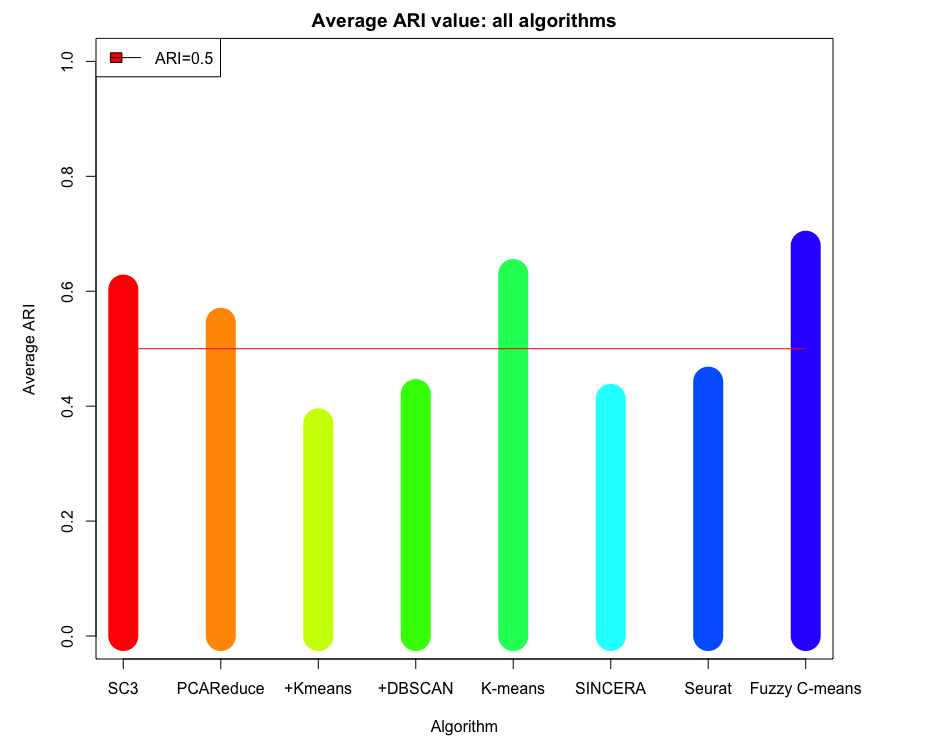
\includegraphics[scale=0.4]{benchmark/ariAverageAll.png}
\caption{Average Adjusted Rand Index (ARI) for some algorithms on Biase, Deng, Goolam, Treutlein, Klein, Ciona, Tintori, Kolodziejczyk, Yan and Usoskin datasets}
\label{averageARI}
\end{figure}

\begin{figure}[H]
\centering
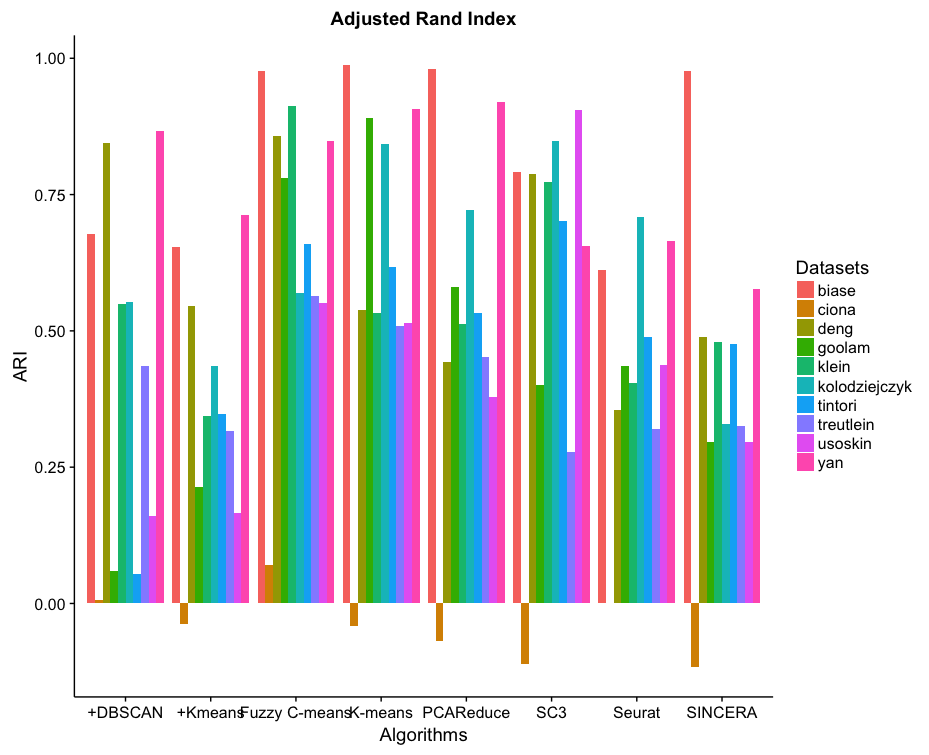
\includegraphics[scale=0.4]{benchmark/ariAll.png}
\caption{Average Adjusted Rand Index (ARI) for some algorithms on Biase, Deng, Goolam, Treutlein, Klein, Ciona, Tintori, Kolodziejczyk, Yan and Usoskin datasets}
\label{averageARI}
\end{figure}

\begin{figure}[H]
\centering
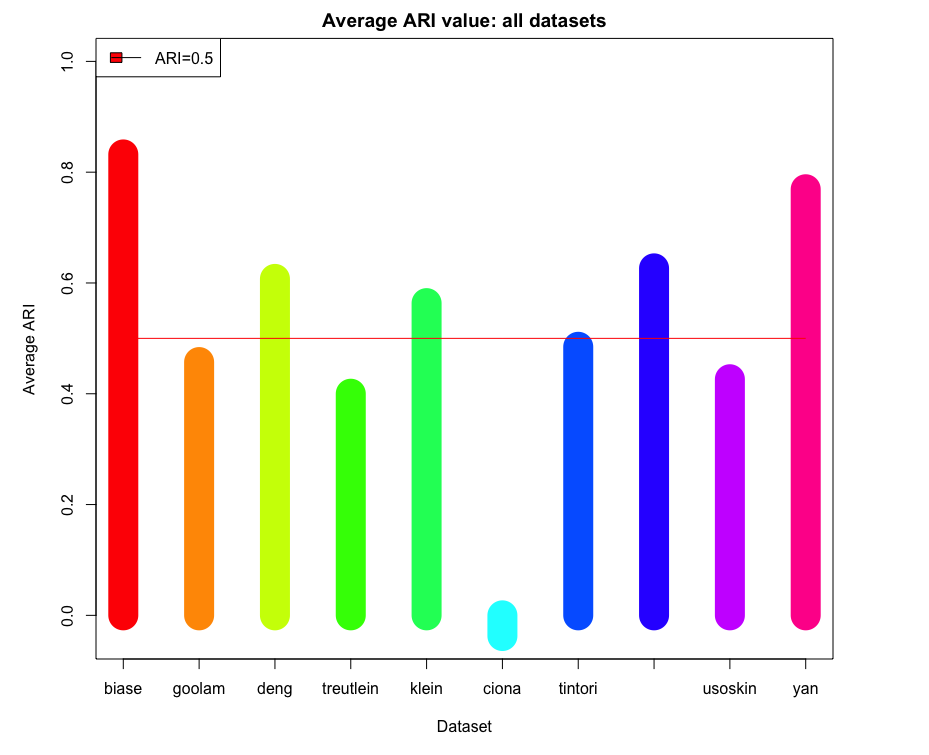
\includegraphics[scale=0.35]{benchmark/ariAverageAllDatasets.png}
\caption{Average ARI for all tested algorithms per dataset}
\label{ariDataset}
\end{figure}

%%TODO comments on accuracy

\bigskip
\noindent \textbf{Stability of the clusterings}
\bigskip

The functions used to generate the following plots and compute the stability measure can be found in the benchmark files, at: {\url{https://github.com/oist-gene-clustering/geneclusteringbenchmark}}\\

The chosen stability measure is the frequency of the most frequent solution, as done in \cite{kiselev2016sc3}.

\begin{figure}[H]
\centering
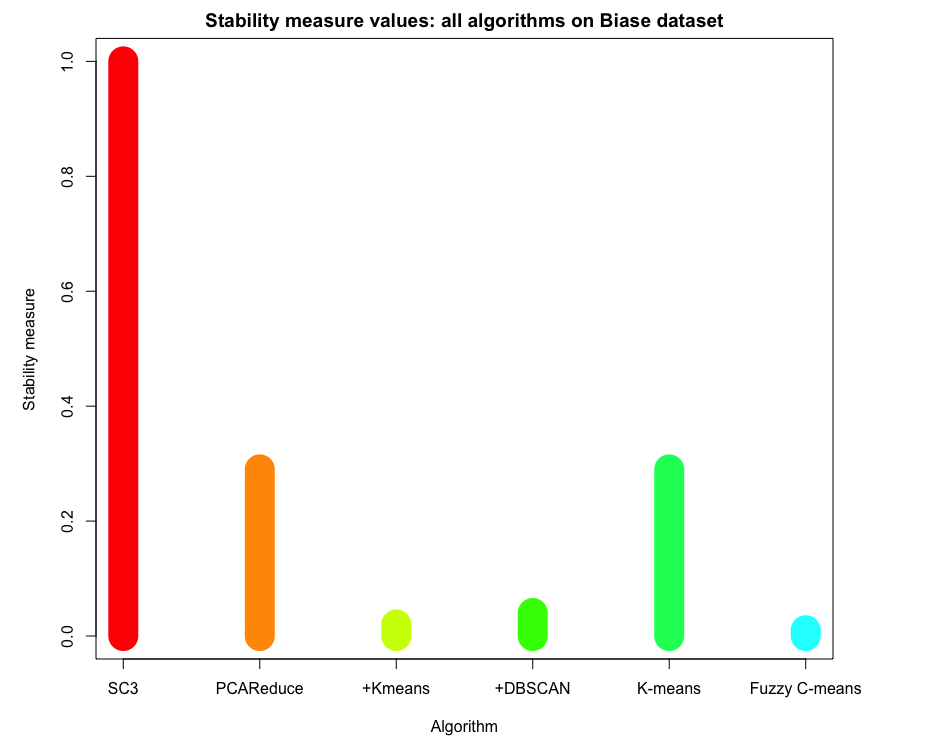
\includegraphics[scale=0.4]{benchmark/stabilityOne.png}
\caption{Stability measure for each algorithm on the Biase dataset, which is the one having the highest mean ARI value overall datasets}
\label{stability}
\end{figure}

But not only it is important to know if the algorithm often returns the same solution, but also knowing how much the returned solutions vary respect to the reference clustering is useful to interpret the correctness of the result. Boxplots help in visualizing quickly the variation of a given measure. 

\begin{figure}[H]
\centering
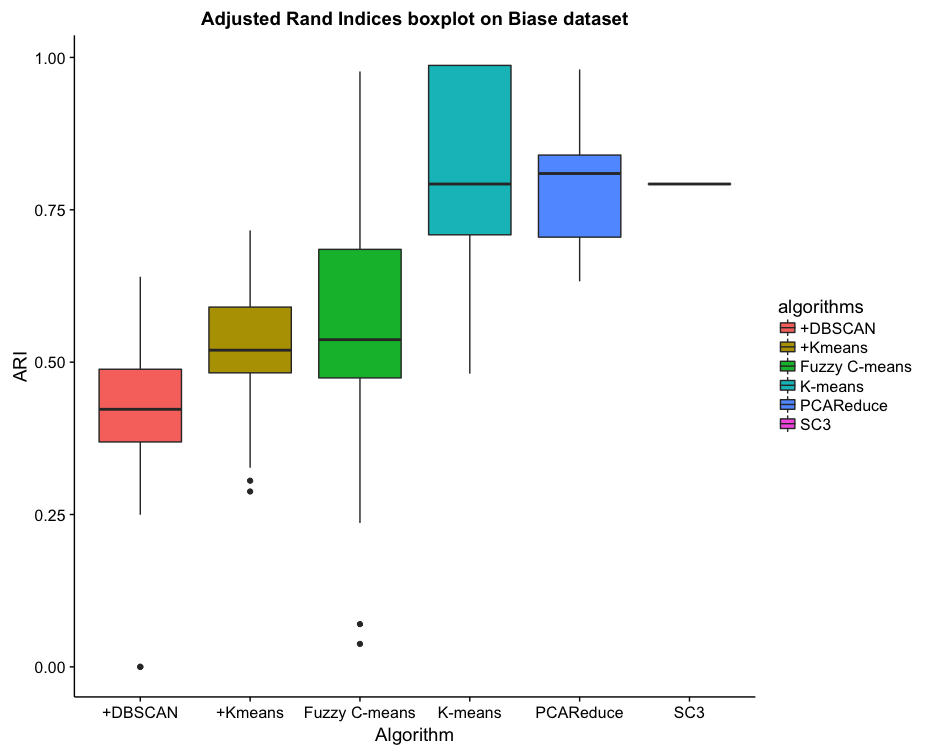
\includegraphics[scale=0.4]{benchmark/boxplotStability.png}
\caption{Adjusted Rand Index (ARI) boxplot for each algorithm on the Biase dataset}
\label{allBoxplotARI}
\end{figure}

According to \cite{boxplot}, the thick black horizontal line is the median value (50th percentile) of the measure, and the top of the box is the 75th percentile of the values, the bottom the 25th percentile. The set of percentiles are the 99 values that split the range of the values into 100 equal parts. The top of the upper (resp. the bottom of the lower) black vertical line ("whisker") is, by default, either the maximum (resp. minimum) value, either the 75th percentile (resp. the 25th percentile) plus (resp. minus) $\frac{3}{2}$ of the box length -75th percentile minus 25th percentile.

%%TODO comments on stability

\bigskip
\noindent \textbf{Time complexity}
\bigskip

The functions used to generate the following plots can be found in the benchmark files, at: {\url{https://github.com/oist-gene-clustering/geneclusteringbenchmark}}\\

\begin{figure}[H]
\centering
\subfigure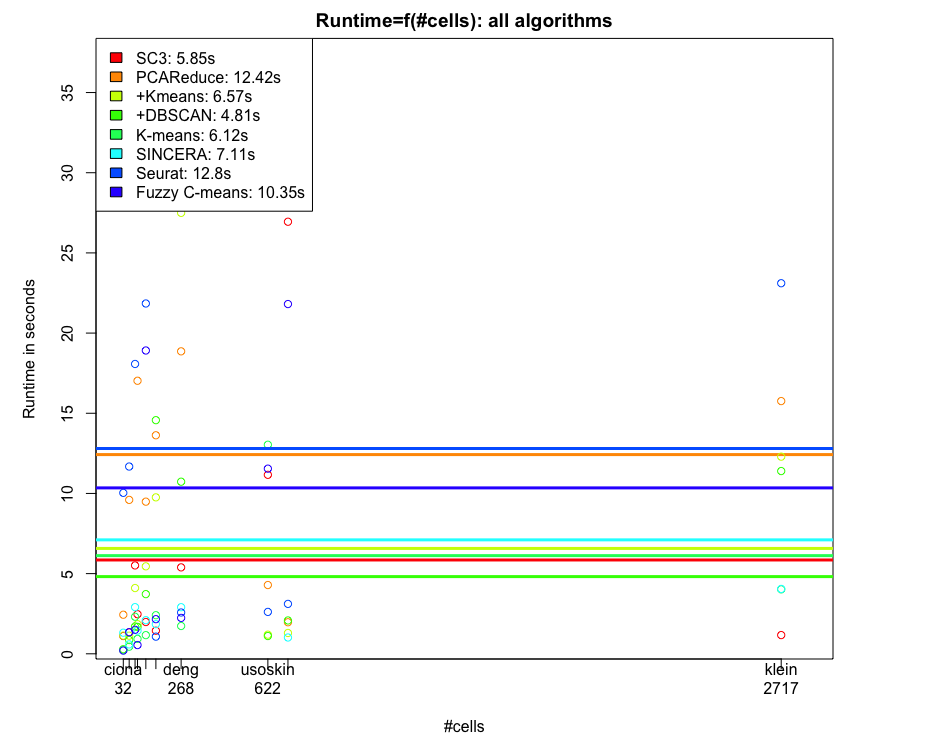
\includegraphics[scale=0.4]{benchmark/timeAllCell.png}
\subfigure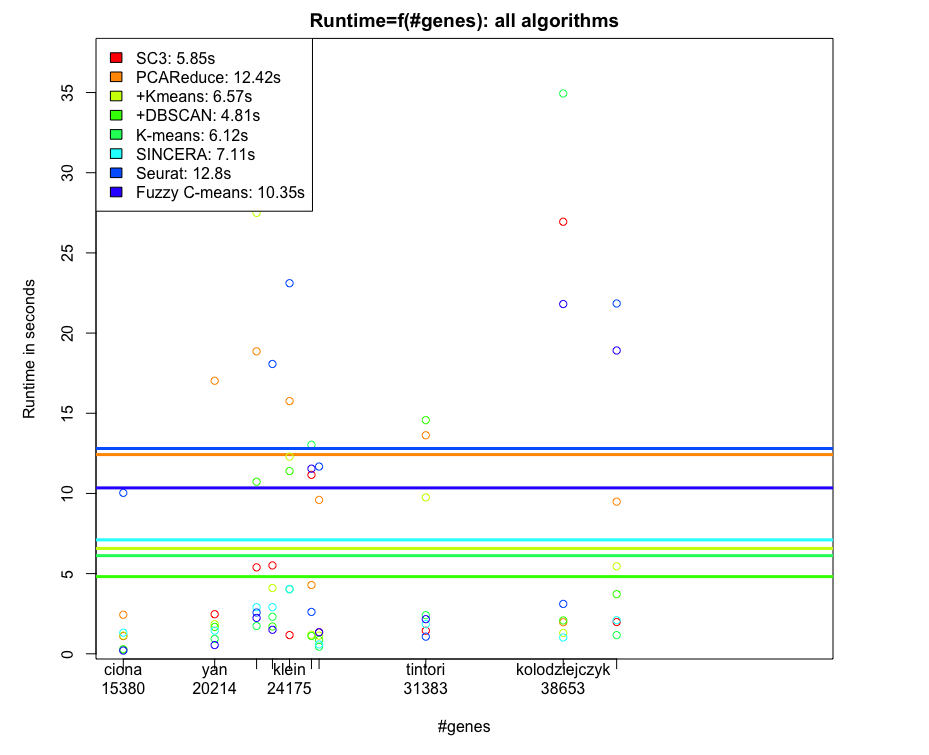
\includegraphics[scale=0.4]{benchmark/timeAllGene.png}
\caption{Time complexity in function of the number of cells (top), of the number of genes (bottom). Lines show the mean runtime for the best solution, for each algorithm across all datasets.}
\label{time1}
\end{figure}

\chapter{Proofs}

\section*{Parametrization equivalences}

\bigskip
\noindent \textbf{Negative-Binomial distribution}
\bigskip

%%TODO

\bigskip
\noindent \textbf{Gamma distribution}
\bigskip

%%TODO

\section*{Model}

%%TODO

\end{document}